\documentclass[12pt,a4paper]{article}

\usepackage[a4paper,text={16.5cm,25.2cm},centering]{geometry}
\usepackage{lmodern}
\usepackage{amssymb,amsmath}
\usepackage{bm}
\usepackage{graphicx}
\usepackage{microtype}
\usepackage{hyperref}
\setlength{\parindent}{0pt}
\setlength{\parskip}{1.2ex}

\hypersetup
       {   pdfauthor = {  },
           pdftitle={  },
           colorlinks=TRUE,
           linkcolor=black,
           citecolor=blue,
           urlcolor=blue
       }




\usepackage{upquote}
\usepackage{listings}
\usepackage{xcolor}
\lstset{
    basicstyle=\ttfamily\footnotesize,
    upquote=true,
    breaklines=true,
    breakindent=0pt,
    keepspaces=true,
    showspaces=false,
    columns=fullflexible,
    showtabs=false,
    showstringspaces=false,
    escapeinside={(*@}{@*)},
    extendedchars=true,
}
\newcommand{\HLJLt}[1]{#1}
\newcommand{\HLJLw}[1]{#1}
\newcommand{\HLJLe}[1]{#1}
\newcommand{\HLJLeB}[1]{#1}
\newcommand{\HLJLo}[1]{#1}
\newcommand{\HLJLk}[1]{\textcolor[RGB]{148,91,176}{\textbf{#1}}}
\newcommand{\HLJLkc}[1]{\textcolor[RGB]{59,151,46}{\textit{#1}}}
\newcommand{\HLJLkd}[1]{\textcolor[RGB]{214,102,97}{\textit{#1}}}
\newcommand{\HLJLkn}[1]{\textcolor[RGB]{148,91,176}{\textbf{#1}}}
\newcommand{\HLJLkp}[1]{\textcolor[RGB]{148,91,176}{\textbf{#1}}}
\newcommand{\HLJLkr}[1]{\textcolor[RGB]{148,91,176}{\textbf{#1}}}
\newcommand{\HLJLkt}[1]{\textcolor[RGB]{148,91,176}{\textbf{#1}}}
\newcommand{\HLJLn}[1]{#1}
\newcommand{\HLJLna}[1]{#1}
\newcommand{\HLJLnb}[1]{#1}
\newcommand{\HLJLnbp}[1]{#1}
\newcommand{\HLJLnc}[1]{#1}
\newcommand{\HLJLncB}[1]{#1}
\newcommand{\HLJLnd}[1]{\textcolor[RGB]{214,102,97}{#1}}
\newcommand{\HLJLne}[1]{#1}
\newcommand{\HLJLneB}[1]{#1}
\newcommand{\HLJLnf}[1]{\textcolor[RGB]{66,102,213}{#1}}
\newcommand{\HLJLnfm}[1]{\textcolor[RGB]{66,102,213}{#1}}
\newcommand{\HLJLnp}[1]{#1}
\newcommand{\HLJLnl}[1]{#1}
\newcommand{\HLJLnn}[1]{#1}
\newcommand{\HLJLno}[1]{#1}
\newcommand{\HLJLnt}[1]{#1}
\newcommand{\HLJLnv}[1]{#1}
\newcommand{\HLJLnvc}[1]{#1}
\newcommand{\HLJLnvg}[1]{#1}
\newcommand{\HLJLnvi}[1]{#1}
\newcommand{\HLJLnvm}[1]{#1}
\newcommand{\HLJLl}[1]{#1}
\newcommand{\HLJLld}[1]{\textcolor[RGB]{148,91,176}{\textit{#1}}}
\newcommand{\HLJLs}[1]{\textcolor[RGB]{201,61,57}{#1}}
\newcommand{\HLJLsa}[1]{\textcolor[RGB]{201,61,57}{#1}}
\newcommand{\HLJLsb}[1]{\textcolor[RGB]{201,61,57}{#1}}
\newcommand{\HLJLsc}[1]{\textcolor[RGB]{201,61,57}{#1}}
\newcommand{\HLJLsd}[1]{\textcolor[RGB]{201,61,57}{#1}}
\newcommand{\HLJLsdB}[1]{\textcolor[RGB]{201,61,57}{#1}}
\newcommand{\HLJLsdC}[1]{\textcolor[RGB]{201,61,57}{#1}}
\newcommand{\HLJLse}[1]{\textcolor[RGB]{59,151,46}{#1}}
\newcommand{\HLJLsh}[1]{\textcolor[RGB]{201,61,57}{#1}}
\newcommand{\HLJLsi}[1]{#1}
\newcommand{\HLJLso}[1]{\textcolor[RGB]{201,61,57}{#1}}
\newcommand{\HLJLsr}[1]{\textcolor[RGB]{201,61,57}{#1}}
\newcommand{\HLJLss}[1]{\textcolor[RGB]{201,61,57}{#1}}
\newcommand{\HLJLssB}[1]{\textcolor[RGB]{201,61,57}{#1}}
\newcommand{\HLJLnB}[1]{\textcolor[RGB]{59,151,46}{#1}}
\newcommand{\HLJLnbB}[1]{\textcolor[RGB]{59,151,46}{#1}}
\newcommand{\HLJLnfB}[1]{\textcolor[RGB]{59,151,46}{#1}}
\newcommand{\HLJLnh}[1]{\textcolor[RGB]{59,151,46}{#1}}
\newcommand{\HLJLni}[1]{\textcolor[RGB]{59,151,46}{#1}}
\newcommand{\HLJLnil}[1]{\textcolor[RGB]{59,151,46}{#1}}
\newcommand{\HLJLnoB}[1]{\textcolor[RGB]{59,151,46}{#1}}
\newcommand{\HLJLoB}[1]{\textcolor[RGB]{102,102,102}{\textbf{#1}}}
\newcommand{\HLJLow}[1]{\textcolor[RGB]{102,102,102}{\textbf{#1}}}
\newcommand{\HLJLp}[1]{#1}
\newcommand{\HLJLc}[1]{\textcolor[RGB]{153,153,119}{\textit{#1}}}
\newcommand{\HLJLch}[1]{\textcolor[RGB]{153,153,119}{\textit{#1}}}
\newcommand{\HLJLcm}[1]{\textcolor[RGB]{153,153,119}{\textit{#1}}}
\newcommand{\HLJLcp}[1]{\textcolor[RGB]{153,153,119}{\textit{#1}}}
\newcommand{\HLJLcpB}[1]{\textcolor[RGB]{153,153,119}{\textit{#1}}}
\newcommand{\HLJLcs}[1]{\textcolor[RGB]{153,153,119}{\textit{#1}}}
\newcommand{\HLJLcsB}[1]{\textcolor[RGB]{153,153,119}{\textit{#1}}}
\newcommand{\HLJLg}[1]{#1}
\newcommand{\HLJLgd}[1]{#1}
\newcommand{\HLJLge}[1]{#1}
\newcommand{\HLJLgeB}[1]{#1}
\newcommand{\HLJLgh}[1]{#1}
\newcommand{\HLJLgi}[1]{#1}
\newcommand{\HLJLgo}[1]{#1}
\newcommand{\HLJLgp}[1]{#1}
\newcommand{\HLJLgs}[1]{#1}
\newcommand{\HLJLgsB}[1]{#1}
\newcommand{\HLJLgt}[1]{#1}


\begin{document}



\section{Fourier methods for periodic functions}
We assume that $f$ is $2\pi$-periodic and its Fourier series converges on $x \in [0, 2\pi)$, i.e.,

\[
f(x) = \sum_{k=-\infty}^{\infty} c_k \mathrm{e}^{\mathrm{i} k x}
\]
where the Fourier coeffients are defined as

\[
%c_k = \frac{1}{2\pi}\int_{-\pi}^{\pi} f(x) \mathrm{e}^{-\mathrm{i}k x} \mathrm{d} x.
c_k = \frac{1}{2\pi}\int_{0}^{2\pi} f(x) \mathrm{e}^{-\mathrm{i}k x} \mathrm{d} x.
\]
Suppose we only know the values of $f(x)$ at the $n$ equally spaced points $x_{j} = jh = \frac{2\pi j}{n}$ for $j = 0, \ldots, n-1$, can we somehow use Fourier series to approximate $f$ and its derivatives?

The idea is to use a truncated Fourier series and approximate Fourier coefficients $\widetilde{c}_k$ to approximate $f$ with

\[
f(x) \approx \sum_{k=-(n-1)/2}^{(n-1)/2} \widetilde{c}_k \mathrm{e}^{\mathrm{i} k x},
\]
assuming $n$ is odd.

\subsection{Trapezoidal rule}
We are going to approximate the Fourier coefficients $c_k$ by using the \emph{trapezoidal rule}.

\textbf{Trapezoidal rule:} Let $x_{j}$, $j = 0, \ldots, n$ be $n+1$ equally spaced points on the interval $[a, b]$. Hence, $x_j = a + jh$ with $h = (b-a)/n$. The $n+1$-point trapezoidal rule for approximating the integral 

\[
I[g] = \int_{a}^{b} g(x) \mathrm{d} x 
\]
is denoted by $I_n[g]$ and defined as

\[
I_n[g] := \frac{h}{2}\left(g(x_0) + 2g(x_1) + 2g(x_2) + \cdots + 2g(x_{n-1}) + g(x_{n})    \right)
\]
The trapezoidal rule is an example of a quadrature method, which are methods to approximate integrals by weighted sums.

Let's use the trapezoidal rule to approximate the Fourier coefficients.  Setting $a = 0$, $b = 2\pi$, $h = 2\pi/n$ and using the fact that $g(x) = f(x)\mathrm{e}^{-\mathrm{i}k x}$ is a $2\pi$-periodic function (since $f(x)$ is assumed to be $2\pi$-periodic), it follows that $g(x_0) = g(x_0 + 2\pi) = g(x_n)$ and we obtain the approximation


\begin{eqnarray*}
c_k &=& \frac{1}{2\pi}\int_{0}^{2\pi} f(x) \mathrm{e}^{-\mathrm{i}k x} \mathrm{d} x \\
    &\approx & \frac{1}{2\pi}I_{n}\left[f\mathrm{e}^{-\mathrm{i}k x}\right]  \\
    &=& \frac{1}{n}\sum_{j = 0}^{n-1} f(x_j)\mathrm{e}^{-\mathrm{i}kx_j} \\
    &:=& \widetilde{c}_k
\end{eqnarray*}
Later we'll see that the trapezoidal rule gives spectacularly accurate approximations to the Fourier coefficients of smooth periodic functions (the approximations $\widetilde{c}_k$ converge exponentially fast to $c_k$ with $n$ for sufficiently smooth functions $f$).  The first step in analysing the accuracy of the approximations $\widetilde{c}_k$ is the following result:

\textbf{Lemma (discrete orthogonality)} For $x_j = jh = \frac{2\pi j}{n}$, we have

\[
I_n\left[\mathrm{e}^{\mathrm{i}kx}\right] = \frac{1}{n}\sum_{j = 0}^{n-1} \mathrm{e}^{\mathrm{i}kx_j} = \begin{cases}
1 & \text{if } k = \ldots, -2n, -n, 0, n, 2n, \ldots \\
0 & \text{otherwise}
\end{cases},
\]
therefore

\[
I_n\left[\mathrm{e}^{\mathrm{i}(k-\ell)x}\right] = \frac{1}{n}\sum_{j = 0}^{n-1} \mathrm{e}^{\mathrm{i}(k-\ell)x_j} = \begin{cases}
1 & \text{if } k-\ell = \ldots, -2n, -n, 0, n, 2n, \ldots \\
0 & \text{otherwise}
\end{cases}.
\]
\textbf{Proof} Case 1: $k = np$, $p \in \mathbb{Z}$, then

\[
\sum_{j = 0}^{n-1} \mathrm{e}^{\mathrm{i}kx_j} = \sum_{j = 0}^{n-1} \mathrm{e}^{2\pi\mathrm{i}kj/n} = \sum_{j = 0}^{n-1} \mathrm{e}^{2\pi\mathrm{i}pj} = \sum_{j = 0}^{n-1} 1 = n.
\]
Case 2: $k \neq np$, $p \in \mathbb{Z}$, then

\[
\sum_{j = 0}^{n-1} \mathrm{e}^{\mathrm{i}kx_j} = \sum_{j = 0}^{n-1} \left(\mathrm{e}^{2\pi\mathrm{i}k/n}\right)^{j} = \frac{1-\left(\mathrm{e}^{2\pi\mathrm{i}k/n}\right)^{n}}{1-\mathrm{e}^{2\pi\mathrm{i}k/n}} = 0,
\]
where we have used the formula

\[
\sum_{j = 0}^{n-1} z^{j} = \frac{1-z^n}{1-z},\qquad z \neq 1,
\]
and the fact that $\mathrm{e}^{2\pi\mathrm{i}k/n} \neq 1$ since $k \neq np$.

\textbf{Corollary} The approximate Fourier coefficients $\widetilde{c}_k$ and the exact Fourier coefficients $c_k$ are related as follows,

\[
\widetilde{c}_k = \cdots + c_{k-2n} + c_{k-n} +  c_k +  c_{k+n} + c_{k+2n} + \cdots
\]
\textbf{Proof}  We have


\begin{eqnarray*}
  \widetilde{c}_k   &=&\frac{1}{n}\sum_{j = 0}^{n-1} f(x_j)\mathrm{e}^{-\mathrm{i}kx_j}   \\
    & = & \frac{1}{n}\sum_{j = 0}^{n-1} \sum_{\ell=-\infty}^{\infty} c_{\ell}\mathrm{e}^{\mathrm{i}\ell x_j} \mathrm{e}^{-\mathrm{i}kx_j}  \\
    &=& \sum_{\ell=-\infty}^{\infty}c_{\ell}\left(\frac{1}{n}\sum_{j = 0}^{n-1} \mathrm{e}^{\mathrm{i}(\ell-k) x_j}   \right)
\end{eqnarray*}
from which the result follows.

Note from the definition of $\widetilde{c}_{k}$ that we have

\[
\widetilde{c}_{k+pn} = \widetilde{c}_{k}, \qquad p \in \mathbb{Z}.  
\]
We can express the approximate Fourier coefficients $\widetilde{c}_k$ as the following matrix vector product:

\[
\underbrace{\left(
\begin{array}{c}
\widetilde{c}_0 \\
\widetilde{c}_1 \\
\vdots \\
\widetilde{c}_{n-2} \\
\widetilde{c}_{n-1}
\end{array}
\right)}_{\widetilde{\mathbf{c}}} = 
{1 \over n} \begin{bmatrix} 1 & 1 & 1&  \ensuremath{\cdots} & 1 \\
                                    1 & {\rm e}^{-{\rm i} x_1} & {\rm e}^{-{\rm i} x_2} & \ensuremath{\cdots} & {\rm e}^{-{\rm i} x_{n-1}} \\
                                    1 & {\rm e}^{-{\rm i} 2 x_1} & {\rm e}^{-{\rm i} 2 x_2} & \ensuremath{\cdots} & {\rm e}^{-{\rm i} 2x_{n-1}} \\
                                    \ensuremath{\vdots} & \ensuremath{\vdots} & \ensuremath{\vdots} & \ensuremath{\ddots} & \ensuremath{\vdots} \\
                                    1 & {\rm e}^{-{\rm i} (n-1) x_1} & {\rm e}^{-{\rm i} (n-1) x_2} & \ensuremath{\cdots} & {\rm e}^{-{\rm i} (n-1) x_{n-1}}
\end{bmatrix} 
\underbrace{\left(
\begin{array}{c}
f(x_0) \\
f(x_1) \\
\vdots \\
f(x_{n-2}) \\
f(x_{n-1})
\end{array}
\right)}_{\mathbf{f}}.
\]
We express this as

\[
\widetilde{\mathbf{c}} = \frac{1}{\sqrt{n}}Q_{n}\mathbf{f}
\]
where $Q_n$ is the \emph{Discrete Fourier Transform} (DFT) matrix.

\textbf{Definition (DFT)} The \emph{Discrete Fourier Transform (DFT)} matrix is defined as:


\begin{align*}
Q_n &:= {1 \over \sqrt{n}} \begin{bmatrix} 1 & 1 & 1&  \ensuremath{\cdots} & 1 \\
                                    1 & {\rm e}^{-{\rm i} x_1} & {\rm e}^{-{\rm i} x_2} & \ensuremath{\cdots} & {\rm e}^{-{\rm i} x_{n-1}} \\
                                    1 & {\rm e}^{-{\rm i} 2 x_1} & {\rm e}^{-{\rm i} 2 x_2} & \ensuremath{\cdots} & {\rm e}^{-{\rm i} 2x_{n-1}} \\
                                    \ensuremath{\vdots} & \ensuremath{\vdots} & \ensuremath{\vdots} & \ensuremath{\ddots} & \ensuremath{\vdots} \\
                                    1 & {\rm e}^{-{\rm i} (n-1) x_1} & {\rm e}^{-{\rm i} (n-1) x_2} & \ensuremath{\cdots} & {\rm e}^{-{\rm i} (n-1) x_{n-1}}
\end{bmatrix} 
\end{align*}
Note that


\begin{align*}
Q_n^\ensuremath{\star} &= {1 \over \sqrt{n}} \begin{bmatrix}
1 & 1 & 1&  \ensuremath{\cdots} & 1 \\
1 & {\rm e}^{{\rm i} x_1} & {\rm e}^{{\rm i} 2 x_1} & \ensuremath{\cdots} & {\rm e}^{{\rm i} (n-1) x_1} \\
1 &  {\rm e}^{{\rm i} x_2}  & {\rm e}^{{\rm i} 2 x_2} & \ensuremath{\cdots} & {\rm e}^{{\rm i} (n-1)x_2} \\
\ensuremath{\vdots} & \ensuremath{\vdots} & \ensuremath{\vdots} & \ensuremath{\ddots} & \ensuremath{\vdots} \\
1 & {\rm e}^{{\rm i} x_{n-1}} & {\rm e}^{{\rm i} 2 x_{n-1}} & \ensuremath{\cdots} & {\rm e}^{{\rm i} (n-1) x_{n-1}}
\end{bmatrix} 
\end{align*}
\textbf{Proposition (DFT is Unitary)} $Q_n$ is unitary: $Q_n^\ensuremath{\star} Q_n = Q_n Q_n^\ensuremath{\star} = I$.

\textbf{Proof}

\[
Q_n Q_n^\ensuremath{\star}  = \begin{bmatrix} I_n[1] & I_n[{\rm e}^{{\rm i} x}] & \ensuremath{\cdots} & I_n[{\rm e}^{{\rm i} (n-1) x}] \\
                            I_n[{\rm e}^{-{\rm i} x}] & I_n[1] & \ensuremath{\cdots} & I_n[{\rm e}^{{\rm i} (n-2) x}] \\
                            \ensuremath{\vdots} & \ensuremath{\vdots} & \ensuremath{\ddots} & \ensuremath{\vdots} \\
                            I_n[{\rm e}^{-{\rm i}(n-1) x}] & I_n[{\rm e}^{-{\rm i}(n-2) x}] & \ensuremath{\cdots} & I_n[1]
                            \end{bmatrix} = I
\]
\[
\blacksquare
\]
\textbf{Proposition (trigonometric interpolant)} Suppose $n$ is odd with $n = 2m+1$, then 

\[
p(x) = \sum_{k=-m}^{m}\widetilde{c}_{k}{\rm e}^{{\rm i}kx}
\]
interpolates $f$ at $x_j$, $j = 0, \ldots, n-1$, i.e., $p(x_j) = f(x_j)$ for $j = 0, \ldots, n-1$.

\textbf{Proof}  We want to show that $\mathbf{p} = \mathbf{f}$, where 

\[
\mathbf{p} = \left(
\begin{array}{c}
p(x_0) \\
p(x_1) \\
\vdots \\
p(x_{n-2}) \\
p(x_{n-1})
\end{array}
\right) \qquad \text{and} \qquad 
\mathbf{f} = \left(
\begin{array}{c}
f(x_0) \\
f(x_1) \\
\vdots \\
f(x_{n-2}) \\
f(x_{n-1})
\end{array}
\right)
\]
We have that

\[
\mathbf{p} = \left(
\begin{array}{c}
p(x_0) \\
p(x_1) \\
\vdots \\
p(x_{n-2}) \\
p(x_{n-1})
\end{array}
\right)
=
\underbrace{\begin{bmatrix}
1 & 1 & 1&  \ensuremath{\cdots} & 1 \\
{\rm e}^{-{\rm i}m x_1} & {\rm e}^{-{\rm i}(m-1) x_1} &  {\rm e}^{-{\rm i}(m-2) x_1} & \ensuremath{\cdots} & {\rm e}^{{\rm i} m x_1} \\
{\rm e}^{-{\rm i}m x_2} & {\rm e}^{-{\rm i}(m-1) x_2} &  {\rm e}^{-{\rm i}(m-2) x_2} & \ensuremath{\cdots} & {\rm e}^{{\rm i} m x_2} \\
\ensuremath{\vdots} & \ensuremath{\vdots} & \ensuremath{\vdots} & \ensuremath{\ddots} & \ensuremath{\vdots} \\
{\rm e}^{-{\rm i}m x_{n-1}}& {\rm e}^{-{\rm i}(m-1)x_{n-1}}& {\rm e}^{-{\rm i}(m-2)x_{n-1}}& \cdots & {\rm e}^{{\rm i}m x_{n-1}}
\end{bmatrix}}_{V} 
\left(
\begin{array}{l}
\widetilde{c}_{-m} \\
\widetilde{c}_{-m+1} \\
\vdots \\
\widetilde{c}_{m-1} \\
\widetilde{c}_{m}
\end{array}
\right)
\]
where $V$ is known as the Vandermonde matrix.

Since $\widetilde{c}_{-1} = \widetilde{c}_{n-1}$, $\widetilde{c}_{-2} = \widetilde{c}_{n-2}$, $\ldots$, $\widetilde{c}_{-m} = \widetilde{c}_{n-m} = \widetilde{c}_{m+1}$

\[
\left(
\begin{array}{l}
\widetilde{c}_{-m} \\
\vdots \\
\widetilde{c}_{m}
\end{array}
\right) = 
\underbrace{\left(
\begin{array}{c c}
   & I_{m} \\
I_{m+1} & 
\end{array}
\right)}_{P}
\left(
\begin{array}{l}
\widetilde{c}_{0} \\
\vdots \\
\widetilde{c}_{n-1}
\end{array}
\right) = P\: \widetilde{\mathbf{c}} = \frac{P}{\sqrt{n}}Q_{n}\mathbf{f}
\]
where $P$ is a permutation matrix.

Let $\mathbf{x} = \left(\begin{array}{c c c} x_0 & \cdots & x_{n-1}  \end{array}\right)^{\top}$, then we can express the Vandermonde matrix as

\[
V = 
\left(
\begin{array}{c c c c c c c}
{\rm e}^{-{\rm i}m\mathbf{x}}  & \cdots & {\rm e}^{-{\rm i}\mathbf{x}} &\mathbf{1}  & {\rm e}^{{\rm i}\mathbf{x}} & \cdots & {\rm e}^{{\rm i}m\mathbf{x}}
\end{array}
\right)
\]
and

\[
\sqrt{n}\,Q_n^* = \left(
\begin{array}{c c c c c}
\mathbf{1}  & {\rm e}^{{\rm i}\mathbf{x}} & {\rm e}^{2{\rm i}\mathbf{x}} & \ldots & {\rm e}^{(n-1){\rm i}\mathbf{x}}
\end{array}
\right)
\]
Since ${\rm e}^{-{\rm i}\mathbf{x}} = {\rm e}^{{\rm i}(n-1)\mathbf{x}}$, ${\rm e}^{-2{\rm i}\mathbf{x}} = {\rm e}^{{\rm i}(n-2)\mathbf{x}}$, $\dots$, ${\rm e}^{-m{\rm i}\mathbf{x}} = {\rm e}^{{\rm i}(n-m)\mathbf{x}} = {\rm e}^{{\rm i}(m+1)\mathbf{x}}$, we have that

\[
V = \sqrt{n}\,Q_n^*\left(
\begin{array}{c c}
 & I_{m+1} \\
I_m &
\end{array}
\right) =  \sqrt{n}\,Q_n^* P^{\top}
\]
Putting everything together, we have

\[
\mathbf{p} = \sqrt{n}Q_n^* P^{T} P \frac{Q_n}{\sqrt{n}}\mathbf{f} = \mathbf{f}
\]
\[
\blacksquare
\]
Let's check the formula $V = \sqrt{n}\,Q_n^* P^{\top}$ in code


\begin{lstlisting}
(*@\HLJLk{using}@*) (*@\HLJLn{Plots}@*)(*@\HLJLp{,}@*) (*@\HLJLn{LinearAlgebra}@*)(*@\HLJLp{,}@*) (*@\HLJLn{SparseArrays}@*)
(*@\HLJLn{n}@*) (*@\HLJLoB{=}@*) (*@\HLJLni{11}@*)
(*@\HLJLn{m}@*) (*@\HLJLoB{=}@*) (*@\HLJLp{(}@*)(*@\HLJLn{n}@*)(*@\HLJLoB{-}@*)(*@\HLJLni{1}@*)(*@\HLJLp{)}@*)(*@\HLJLoB{\ensuremath{\div}}@*)(*@\HLJLni{2}@*)
(*@\HLJLn{x}@*) (*@\HLJLoB{=}@*) (*@\HLJLnf{range}@*)(*@\HLJLp{(}@*)(*@\HLJLni{0}@*)(*@\HLJLp{,}@*)(*@\HLJLni{2}@*)(*@\HLJLn{\ensuremath{\pi}}@*)(*@\HLJLp{;}@*) (*@\HLJLn{length}@*)(*@\HLJLoB{=}@*)(*@\HLJLn{n}@*)(*@\HLJLoB{+}@*)(*@\HLJLni{1}@*)(*@\HLJLp{)[}@*)(*@\HLJLni{1}@*)(*@\HLJLoB{:}@*)(*@\HLJLk{end}@*)(*@\HLJLoB{-}@*)(*@\HLJLni{1}@*)(*@\HLJLp{]}@*) (*@\HLJLcs{{\#}}@*) (*@\HLJLcs{x{\_}0,}@*) (*@\HLJLcs{\ensuremath{\ldots},x{\_}{\{}n-1{\}},}@*) (*@\HLJLcs{dropping}@*) (*@\HLJLcs{x{\_}n}@*) (*@\HLJLcs{==}@*) (*@\HLJLcs{2\ensuremath{\pi}}@*)
(*@\HLJLn{Q\ensuremath{\_n}}@*) (*@\HLJLoB{=}@*) (*@\HLJLp{[}@*)(*@\HLJLnf{exp}@*)(*@\HLJLp{(}@*)(*@\HLJLoB{-}@*)(*@\HLJLn{im}@*)(*@\HLJLoB{*}@*)(*@\HLJLp{(}@*)(*@\HLJLn{k}@*)(*@\HLJLoB{-}@*)(*@\HLJLni{1}@*)(*@\HLJLp{)}@*)(*@\HLJLoB{*}@*)(*@\HLJLn{x}@*)(*@\HLJLp{[}@*)(*@\HLJLn{j}@*)(*@\HLJLp{])}@*) (*@\HLJLk{for}@*) (*@\HLJLn{k}@*) (*@\HLJLoB{=}@*) (*@\HLJLni{1}@*)(*@\HLJLoB{:}@*)(*@\HLJLn{n}@*)(*@\HLJLp{,}@*) (*@\HLJLn{j}@*)(*@\HLJLoB{=}@*)(*@\HLJLni{1}@*)(*@\HLJLoB{:}@*)(*@\HLJLn{n}@*)(*@\HLJLp{]}@*)(*@\HLJLoB{/}@*)(*@\HLJLnf{sqrt}@*)(*@\HLJLp{(}@*)(*@\HLJLn{n}@*)(*@\HLJLp{)}@*)
(*@\HLJLn{Q\ensuremath{\_n}}@*)(*@\HLJLoB{*}@*)(*@\HLJLn{Q\ensuremath{\_n}}@*)(*@\HLJLoB{{\textquotesingle}}@*) (*@\HLJLoB{\ensuremath{\approx}}@*) (*@\HLJLn{I}@*)
\end{lstlisting}

\begin{lstlisting}
true
\end{lstlisting}


\begin{lstlisting}
(*@\HLJLn{P}@*) (*@\HLJLoB{=}@*) (*@\HLJLnf{sparse}@*)(*@\HLJLp{(}@*)(*@\HLJLni{1}@*)(*@\HLJLoB{:}@*)(*@\HLJLn{n}@*)(*@\HLJLp{,}@*) (*@\HLJLp{[}@*)(*@\HLJLn{m}@*)(*@\HLJLoB{+}@*)(*@\HLJLni{2}@*)(*@\HLJLoB{:}@*)(*@\HLJLn{n}@*)(*@\HLJLp{;}@*)(*@\HLJLni{1}@*)(*@\HLJLoB{:}@*)(*@\HLJLn{m}@*)(*@\HLJLoB{+}@*)(*@\HLJLni{1}@*)(*@\HLJLp{],}@*) (*@\HLJLnf{fill}@*)(*@\HLJLp{(}@*)(*@\HLJLni{1}@*)(*@\HLJLp{,}@*)(*@\HLJLn{n}@*)(*@\HLJLp{))}@*)
\end{lstlisting}

\begin{lstlisting}
11(*@\ensuremath{\times}@*)11 SparseMatrixCSC(*@{{\{}}@*)Int64, Int64(*@{{\}}}@*) with 11 stored entries:
 (*@\ensuremath{\cdot}@*)  (*@\ensuremath{\cdot}@*)  (*@\ensuremath{\cdot}@*)  (*@\ensuremath{\cdot}@*)  (*@\ensuremath{\cdot}@*)  (*@\ensuremath{\cdot}@*)  1  (*@\ensuremath{\cdot}@*)  (*@\ensuremath{\cdot}@*)  (*@\ensuremath{\cdot}@*)  (*@\ensuremath{\cdot}@*)
 (*@\ensuremath{\cdot}@*)  (*@\ensuremath{\cdot}@*)  (*@\ensuremath{\cdot}@*)  (*@\ensuremath{\cdot}@*)  (*@\ensuremath{\cdot}@*)  (*@\ensuremath{\cdot}@*)  (*@\ensuremath{\cdot}@*)  1  (*@\ensuremath{\cdot}@*)  (*@\ensuremath{\cdot}@*)  (*@\ensuremath{\cdot}@*)
 (*@\ensuremath{\cdot}@*)  (*@\ensuremath{\cdot}@*)  (*@\ensuremath{\cdot}@*)  (*@\ensuremath{\cdot}@*)  (*@\ensuremath{\cdot}@*)  (*@\ensuremath{\cdot}@*)  (*@\ensuremath{\cdot}@*)  (*@\ensuremath{\cdot}@*)  1  (*@\ensuremath{\cdot}@*)  (*@\ensuremath{\cdot}@*)
 (*@\ensuremath{\cdot}@*)  (*@\ensuremath{\cdot}@*)  (*@\ensuremath{\cdot}@*)  (*@\ensuremath{\cdot}@*)  (*@\ensuremath{\cdot}@*)  (*@\ensuremath{\cdot}@*)  (*@\ensuremath{\cdot}@*)  (*@\ensuremath{\cdot}@*)  (*@\ensuremath{\cdot}@*)  1  (*@\ensuremath{\cdot}@*)
 (*@\ensuremath{\cdot}@*)  (*@\ensuremath{\cdot}@*)  (*@\ensuremath{\cdot}@*)  (*@\ensuremath{\cdot}@*)  (*@\ensuremath{\cdot}@*)  (*@\ensuremath{\cdot}@*)  (*@\ensuremath{\cdot}@*)  (*@\ensuremath{\cdot}@*)  (*@\ensuremath{\cdot}@*)  (*@\ensuremath{\cdot}@*)  1
 1  (*@\ensuremath{\cdot}@*)  (*@\ensuremath{\cdot}@*)  (*@\ensuremath{\cdot}@*)  (*@\ensuremath{\cdot}@*)  (*@\ensuremath{\cdot}@*)  (*@\ensuremath{\cdot}@*)  (*@\ensuremath{\cdot}@*)  (*@\ensuremath{\cdot}@*)  (*@\ensuremath{\cdot}@*)  (*@\ensuremath{\cdot}@*)
 (*@\ensuremath{\cdot}@*)  1  (*@\ensuremath{\cdot}@*)  (*@\ensuremath{\cdot}@*)  (*@\ensuremath{\cdot}@*)  (*@\ensuremath{\cdot}@*)  (*@\ensuremath{\cdot}@*)  (*@\ensuremath{\cdot}@*)  (*@\ensuremath{\cdot}@*)  (*@\ensuremath{\cdot}@*)  (*@\ensuremath{\cdot}@*)
 (*@\ensuremath{\cdot}@*)  (*@\ensuremath{\cdot}@*)  1  (*@\ensuremath{\cdot}@*)  (*@\ensuremath{\cdot}@*)  (*@\ensuremath{\cdot}@*)  (*@\ensuremath{\cdot}@*)  (*@\ensuremath{\cdot}@*)  (*@\ensuremath{\cdot}@*)  (*@\ensuremath{\cdot}@*)  (*@\ensuremath{\cdot}@*)
 (*@\ensuremath{\cdot}@*)  (*@\ensuremath{\cdot}@*)  (*@\ensuremath{\cdot}@*)  1  (*@\ensuremath{\cdot}@*)  (*@\ensuremath{\cdot}@*)  (*@\ensuremath{\cdot}@*)  (*@\ensuremath{\cdot}@*)  (*@\ensuremath{\cdot}@*)  (*@\ensuremath{\cdot}@*)  (*@\ensuremath{\cdot}@*)
 (*@\ensuremath{\cdot}@*)  (*@\ensuremath{\cdot}@*)  (*@\ensuremath{\cdot}@*)  (*@\ensuremath{\cdot}@*)  1  (*@\ensuremath{\cdot}@*)  (*@\ensuremath{\cdot}@*)  (*@\ensuremath{\cdot}@*)  (*@\ensuremath{\cdot}@*)  (*@\ensuremath{\cdot}@*)  (*@\ensuremath{\cdot}@*)
 (*@\ensuremath{\cdot}@*)  (*@\ensuremath{\cdot}@*)  (*@\ensuremath{\cdot}@*)  (*@\ensuremath{\cdot}@*)  (*@\ensuremath{\cdot}@*)  1  (*@\ensuremath{\cdot}@*)  (*@\ensuremath{\cdot}@*)  (*@\ensuremath{\cdot}@*)  (*@\ensuremath{\cdot}@*)  (*@\ensuremath{\cdot}@*)
\end{lstlisting}


\begin{lstlisting}
(*@\HLJLn{V}@*) (*@\HLJLoB{=}@*) (*@\HLJLp{[}@*)(*@\HLJLnf{exp}@*)(*@\HLJLp{(}@*)(*@\HLJLn{im}@*)(*@\HLJLoB{*}@*)(*@\HLJLn{k}@*)(*@\HLJLoB{*}@*)(*@\HLJLn{x}@*)(*@\HLJLp{[}@*)(*@\HLJLn{j}@*)(*@\HLJLp{])}@*) (*@\HLJLk{for}@*) (*@\HLJLn{j}@*) (*@\HLJLoB{=}@*) (*@\HLJLni{1}@*)(*@\HLJLoB{:}@*)(*@\HLJLn{n}@*)(*@\HLJLp{,}@*) (*@\HLJLn{k}@*)(*@\HLJLoB{=-}@*)(*@\HLJLn{m}@*)(*@\HLJLoB{:}@*)(*@\HLJLn{m}@*)(*@\HLJLp{]}@*)
(*@\HLJLn{V}@*) (*@\HLJLoB{\ensuremath{\approx}}@*) (*@\HLJLnf{sqrt}@*)(*@\HLJLp{(}@*)(*@\HLJLn{n}@*)(*@\HLJLp{)}@*)(*@\HLJLoB{*}@*)(*@\HLJLn{Q\ensuremath{\_n}}@*)(*@\HLJLoB{{\textquotesingle}*}@*)(*@\HLJLnf{transpose}@*)(*@\HLJLp{(}@*)(*@\HLJLn{P}@*)(*@\HLJLp{)}@*)
\end{lstlisting}

\begin{lstlisting}
true
\end{lstlisting}


Here's an example illustrating that $p(x)$ interpolates $f$ at $x_{j}$ for $j = 0, \ldots, n-1$.


\begin{lstlisting}
(*@\HLJLcs{{\#}}@*) (*@\HLJLcs{write}@*) (*@\HLJLcs{a}@*) (*@\HLJLcs{function}@*) (*@\HLJLcs{that}@*) (*@\HLJLcs{evaluates}@*) (*@\HLJLcs{the}@*) (*@\HLJLcs{interpolant}@*)
(*@\HLJLk{function}@*) (*@\HLJLnf{triginterp}@*)(*@\HLJLp{(}@*)(*@\HLJLn{c}@*)(*@\HLJLp{,}@*) (*@\HLJLn{x}@*)(*@\HLJLp{)}@*)
    (*@\HLJLcs{{\#}}@*) (*@\HLJLcs{ct}@*) (*@\HLJLcs{=}@*) (*@\HLJLcs{[c\ensuremath{\_0},}@*) (*@\HLJLcs{\ensuremath{\ldots},}@*) (*@\HLJLcs{c\ensuremath{\_n}\ensuremath{\_-}\ensuremath{\_1}]}@*) (*@\HLJLcs{(the}@*) (*@\HLJLcs{approximate}@*) (*@\HLJLcs{Fourier}@*) (*@\HLJLcs{coefficients)}@*)
    (*@\HLJLn{m}@*) (*@\HLJLoB{=}@*) (*@\HLJLp{(}@*)(*@\HLJLn{n}@*)(*@\HLJLoB{-}@*)(*@\HLJLni{1}@*)(*@\HLJLp{)}@*)(*@\HLJLoB{\ensuremath{\div}}@*)(*@\HLJLni{2}@*) (*@\HLJLcs{{\#}}@*) (*@\HLJLcs{use}@*) (*@\HLJLcs{coefficients}@*) (*@\HLJLcs{between}@*) (*@\HLJLcs{-m:m}@*)
    (*@\HLJLn{p}@*) (*@\HLJLoB{=}@*) (*@\HLJLnfB{0.0}@*) (*@\HLJLoB{+}@*) (*@\HLJLnfB{0.0}@*)(*@\HLJLn{im}@*) (*@\HLJLcs{{\#}}@*) (*@\HLJLcs{coefficients}@*) (*@\HLJLcs{are}@*) (*@\HLJLcs{complex}@*) (*@\HLJLcs{so}@*) (*@\HLJLcs{we}@*) (*@\HLJLcs{need}@*) (*@\HLJLcs{complex}@*) (*@\HLJLcs{arithmetic}@*)
    (*@\HLJLk{for}@*) (*@\HLJLn{k}@*) (*@\HLJLoB{=}@*) (*@\HLJLni{0}@*)(*@\HLJLoB{:}@*)(*@\HLJLn{m}@*)
        (*@\HLJLn{p}@*) (*@\HLJLoB{+=}@*) (*@\HLJLn{c}@*)(*@\HLJLp{[}@*)(*@\HLJLn{k}@*)(*@\HLJLoB{+}@*)(*@\HLJLni{1}@*)(*@\HLJLp{]}@*) (*@\HLJLoB{*}@*) (*@\HLJLnf{exp}@*)(*@\HLJLp{(}@*)(*@\HLJLn{im}@*)(*@\HLJLoB{*}@*)(*@\HLJLn{k}@*)(*@\HLJLoB{*}@*)(*@\HLJLn{x}@*)(*@\HLJLp{)}@*)
    (*@\HLJLk{end}@*)
    (*@\HLJLk{for}@*) (*@\HLJLn{k}@*) (*@\HLJLoB{=}@*) (*@\HLJLoB{-}@*)(*@\HLJLn{m}@*)(*@\HLJLoB{:-}@*)(*@\HLJLni{1}@*)
        (*@\HLJLn{p}@*) (*@\HLJLoB{+=}@*) (*@\HLJLn{c}@*)(*@\HLJLp{[}@*)(*@\HLJLk{end}@*)(*@\HLJLoB{+}@*)(*@\HLJLn{k}@*)(*@\HLJLoB{+}@*)(*@\HLJLni{1}@*)(*@\HLJLp{]}@*) (*@\HLJLoB{*}@*) (*@\HLJLnf{exp}@*)(*@\HLJLp{(}@*)(*@\HLJLn{im}@*)(*@\HLJLoB{*}@*)(*@\HLJLn{k}@*)(*@\HLJLoB{*}@*)(*@\HLJLn{x}@*)(*@\HLJLp{)}@*)
    (*@\HLJLk{end}@*)
    (*@\HLJLn{p}@*)
(*@\HLJLk{end}@*)(*@\HLJLp{;}@*)
\end{lstlisting}


\begin{lstlisting}
(*@\HLJLn{f}@*) (*@\HLJLoB{=}@*) (*@\HLJLn{x}@*) (*@\HLJLoB{->}@*) (*@\HLJLnf{exp}@*)(*@\HLJLp{(}@*)(*@\HLJLnf{cos}@*)(*@\HLJLp{(}@*)(*@\HLJLn{x}@*)(*@\HLJLp{))}@*)
(*@\HLJLn{n}@*) (*@\HLJLoB{=}@*) (*@\HLJLni{5}@*)
(*@\HLJLcs{{\#}}@*) (*@\HLJLcs{compute}@*) (*@\HLJLcs{the}@*) (*@\HLJLcs{approximate}@*) (*@\HLJLcs{Fourier}@*) (*@\HLJLcs{coefficients}@*)
(*@\HLJLn{x}@*) (*@\HLJLoB{=}@*) (*@\HLJLnf{range}@*)(*@\HLJLp{(}@*)(*@\HLJLni{0}@*)(*@\HLJLp{,}@*)(*@\HLJLni{2}@*)(*@\HLJLn{\ensuremath{\pi}}@*)(*@\HLJLp{;}@*) (*@\HLJLn{length}@*)(*@\HLJLoB{=}@*)(*@\HLJLn{n}@*)(*@\HLJLoB{+}@*)(*@\HLJLni{1}@*)(*@\HLJLp{)[}@*)(*@\HLJLni{1}@*)(*@\HLJLoB{:}@*)(*@\HLJLk{end}@*)(*@\HLJLoB{-}@*)(*@\HLJLni{1}@*)(*@\HLJLp{]}@*) (*@\HLJLcs{{\#}}@*) (*@\HLJLcs{interpolation}@*) (*@\HLJLcs{nodes}@*) (*@\HLJLcs{x{\_}0,}@*) (*@\HLJLcs{\ensuremath{\ldots},x{\_}{\{}n-1{\}}}@*)
(*@\HLJLn{Q\ensuremath{\_n}}@*) (*@\HLJLoB{=}@*) (*@\HLJLni{1}@*)(*@\HLJLoB{/}@*)(*@\HLJLnf{sqrt}@*)(*@\HLJLp{(}@*)(*@\HLJLn{n}@*)(*@\HLJLp{)}@*) (*@\HLJLoB{*}@*) (*@\HLJLp{[}@*)(*@\HLJLnf{exp}@*)(*@\HLJLp{(}@*)(*@\HLJLoB{-}@*)(*@\HLJLn{im}@*)(*@\HLJLoB{*}@*)(*@\HLJLp{(}@*)(*@\HLJLn{k}@*)(*@\HLJLoB{-}@*)(*@\HLJLni{1}@*)(*@\HLJLp{)}@*)(*@\HLJLoB{*}@*)(*@\HLJLn{x}@*)(*@\HLJLp{[}@*)(*@\HLJLn{j}@*)(*@\HLJLp{])}@*) (*@\HLJLk{for}@*) (*@\HLJLn{k}@*) (*@\HLJLoB{=}@*) (*@\HLJLni{1}@*)(*@\HLJLoB{:}@*)(*@\HLJLn{n}@*)(*@\HLJLp{,}@*) (*@\HLJLn{j}@*)(*@\HLJLoB{=}@*)(*@\HLJLni{1}@*)(*@\HLJLoB{:}@*)(*@\HLJLn{n}@*)(*@\HLJLp{]}@*)
(*@\HLJLn{c}@*) (*@\HLJLoB{=}@*) (*@\HLJLni{1}@*)(*@\HLJLoB{/}@*)(*@\HLJLnf{sqrt}@*)(*@\HLJLp{(}@*)(*@\HLJLn{n}@*)(*@\HLJLp{)}@*) (*@\HLJLoB{*}@*) (*@\HLJLn{Q\ensuremath{\_n}}@*) (*@\HLJLoB{*}@*) (*@\HLJLn{f}@*)(*@\HLJLoB{.}@*)(*@\HLJLp{(}@*)(*@\HLJLn{x}@*)(*@\HLJLp{)}@*)

(*@\HLJLn{p}@*) (*@\HLJLoB{=}@*) (*@\HLJLn{x}@*) (*@\HLJLoB{->}@*) (*@\HLJLnf{triginterp}@*)(*@\HLJLp{(}@*)(*@\HLJLn{c}@*)(*@\HLJLp{,}@*) (*@\HLJLn{x}@*)(*@\HLJLp{)}@*)

(*@\HLJLn{xx}@*) (*@\HLJLoB{=}@*) (*@\HLJLnf{range}@*)(*@\HLJLp{(}@*)(*@\HLJLni{0}@*)(*@\HLJLp{,}@*) (*@\HLJLni{2}@*)(*@\HLJLn{\ensuremath{\pi}}@*)(*@\HLJLp{;}@*) (*@\HLJLn{length}@*)(*@\HLJLoB{=}@*)(*@\HLJLni{1000}@*)(*@\HLJLp{)}@*) (*@\HLJLcs{{\#}}@*) (*@\HLJLcs{plotting}@*) (*@\HLJLcs{grid}@*)
(*@\HLJLnf{plot}@*)(*@\HLJLp{(}@*)(*@\HLJLn{xx}@*)(*@\HLJLp{,}@*) (*@\HLJLn{f}@*)(*@\HLJLoB{.}@*)(*@\HLJLp{(}@*)(*@\HLJLn{xx}@*)(*@\HLJLp{);}@*) (*@\HLJLn{lw}@*)(*@\HLJLoB{=}@*)(*@\HLJLni{2}@*)(*@\HLJLp{,}@*) (*@\HLJLn{label}@*)(*@\HLJLoB{=}@*)(*@\HLJLs{"{}function"{}}@*)(*@\HLJLp{,}@*)(*@\HLJLn{legend}@*)(*@\HLJLoB{=:}@*)(*@\HLJLn{topright}@*)(*@\HLJLp{)}@*)
(*@\HLJLnf{plot!}@*)(*@\HLJLp{(}@*)(*@\HLJLn{xx}@*)(*@\HLJLp{,}@*) (*@\HLJLn{real}@*)(*@\HLJLoB{.}@*)(*@\HLJLp{(}@*)(*@\HLJLn{p}@*)(*@\HLJLoB{.}@*)(*@\HLJLp{(}@*)(*@\HLJLn{xx}@*)(*@\HLJLp{));}@*) (*@\HLJLn{lw}@*)(*@\HLJLoB{=}@*)(*@\HLJLni{2}@*)(*@\HLJLp{,}@*) (*@\HLJLn{label}@*)(*@\HLJLoB{=}@*)(*@\HLJLs{"{}trigonometric}@*) (*@\HLJLs{interpolant"{}}@*)(*@\HLJLp{)}@*)
(*@\HLJLnf{scatter!}@*)(*@\HLJLp{(}@*)(*@\HLJLn{x}@*)(*@\HLJLp{,}@*) (*@\HLJLn{f}@*)(*@\HLJLoB{.}@*)(*@\HLJLp{(}@*)(*@\HLJLn{x}@*)(*@\HLJLp{);}@*) (*@\HLJLn{label}@*)(*@\HLJLoB{=}@*)(*@\HLJLs{"{}samples"{}}@*)(*@\HLJLp{)}@*)
\end{lstlisting}

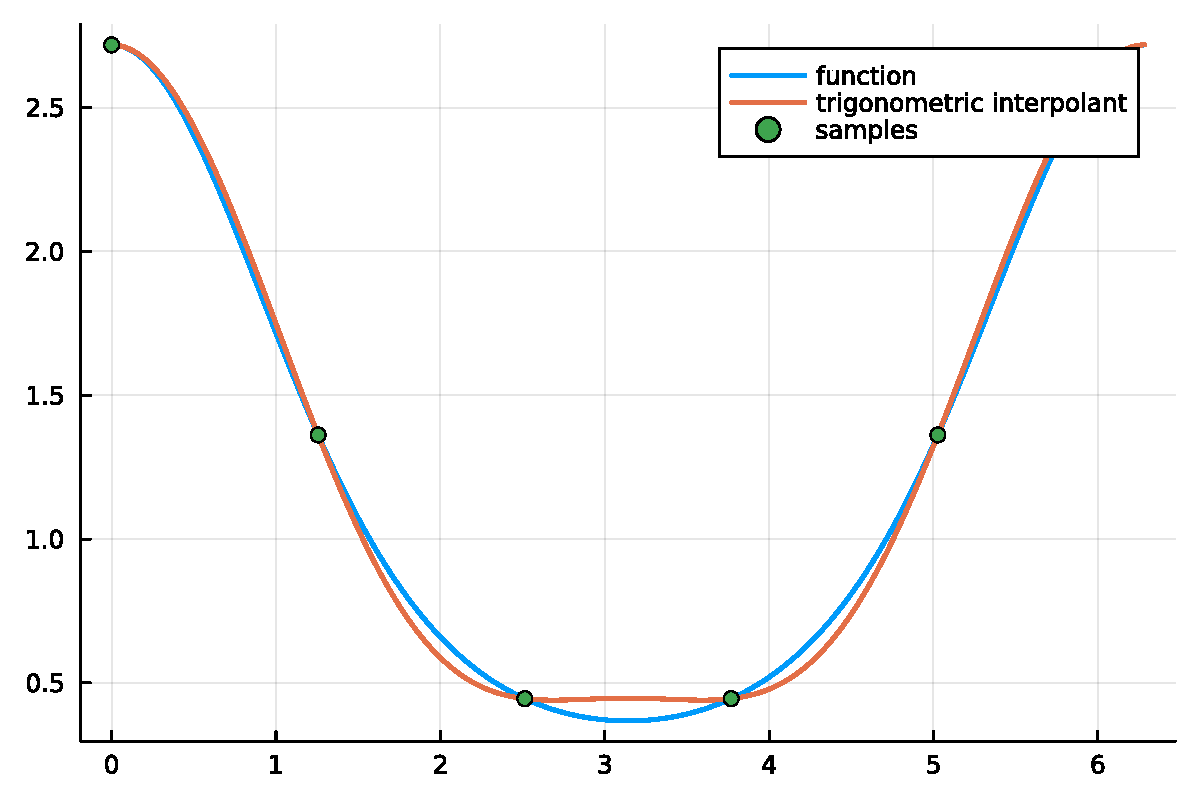
\includegraphics[width=\linewidth]{jl_fFQb2q/Fourier_5_1.pdf}

Applying $Q\ensuremath{\_n}$ or its conjugate transpose $Q_n^\ensuremath{\star}$ to a vector naively takes $\mathcal{O}(n^2)$ operations. Both can be reduced to $\mathcal{O}(n \log n)$ operations using the celebrated \emph{Fast Fourier Transform} (FFT), which is one of the \href{https://pi.math.cornell.edu/~web6140/}{Top 10 Algorithms of the 20th Century}.


\begin{lstlisting}
(*@\HLJLcs{{\#}}@*) (*@\HLJLcs{Here{\textquotesingle}s}@*) (*@\HLJLcs{an}@*) (*@\HLJLcs{example}@*) (*@\HLJLcs{of}@*) (*@\HLJLcs{using}@*) (*@\HLJLcs{the}@*) (*@\HLJLcs{FFT}@*) (*@\HLJLcs{to}@*) (*@\HLJLcs{map}@*) (*@\HLJLcs{function}@*) (*@\HLJLcs{values}@*) (*@\HLJLcs{to}@*) (*@\HLJLcs{coefficients}@*) (*@\HLJLcs{and}@*) (*@\HLJLcs{vice}@*) (*@\HLJLcs{versa}@*)
(*@\HLJLk{using}@*) (*@\HLJLn{FFTW}@*)
(*@\HLJLn{f}@*) (*@\HLJLoB{=}@*) (*@\HLJLn{x}@*) (*@\HLJLoB{->}@*) (*@\HLJLnf{exp}@*)(*@\HLJLp{(}@*)(*@\HLJLnf{cos}@*)(*@\HLJLp{(}@*)(*@\HLJLn{x}@*)(*@\HLJLoB{-}@*)(*@\HLJLnfB{0.1}@*)(*@\HLJLp{))}@*)
(*@\HLJLn{n}@*) (*@\HLJLoB{=}@*) (*@\HLJLni{31}@*)
(*@\HLJLn{m}@*) (*@\HLJLoB{=}@*) (*@\HLJLp{(}@*)(*@\HLJLn{n}@*)(*@\HLJLoB{-}@*)(*@\HLJLni{1}@*)(*@\HLJLp{)}@*)(*@\HLJLoB{\ensuremath{\div}}@*)(*@\HLJLni{2}@*)
(*@\HLJLcs{{\#}}@*) (*@\HLJLcs{evenly}@*) (*@\HLJLcs{spaced}@*) (*@\HLJLcs{points}@*) (*@\HLJLcs{from}@*) (*@\HLJLcs{0:2\ensuremath{\pi},}@*) (*@\HLJLcs{dropping}@*) (*@\HLJLcs{last}@*) (*@\HLJLcs{node}@*)
(*@\HLJLn{x}@*) (*@\HLJLoB{=}@*) (*@\HLJLnf{range}@*)(*@\HLJLp{(}@*)(*@\HLJLni{0}@*)(*@\HLJLp{,}@*) (*@\HLJLni{2}@*)(*@\HLJLn{\ensuremath{\pi}}@*)(*@\HLJLp{;}@*) (*@\HLJLn{length}@*)(*@\HLJLoB{=}@*)(*@\HLJLn{n}@*)(*@\HLJLoB{+}@*)(*@\HLJLni{1}@*)(*@\HLJLp{)[}@*)(*@\HLJLni{1}@*)(*@\HLJLoB{:}@*)(*@\HLJLk{end}@*)(*@\HLJLoB{-}@*)(*@\HLJLni{1}@*)(*@\HLJLp{]}@*)
(*@\HLJLcs{{\#}}@*) (*@\HLJLcs{fft}@*) (*@\HLJLcs{returns}@*) (*@\HLJLcs{the}@*) (*@\HLJLcs{approximate}@*) (*@\HLJLcs{Fourier}@*) (*@\HLJLcs{coefficients}@*) (*@\HLJLcs{n*[c\ensuremath{\_0},}@*) (*@\HLJLcs{\ensuremath{\ldots},}@*) (*@\HLJLcs{c{\_}\ensuremath{\_n}\ensuremath{\_-}\ensuremath{\_1}]}@*)
(*@\HLJLn{c}@*) (*@\HLJLoB{=}@*) (*@\HLJLnf{fft}@*)(*@\HLJLp{(}@*)(*@\HLJLn{f}@*)(*@\HLJLoB{.}@*)(*@\HLJLp{(}@*)(*@\HLJLn{x}@*)(*@\HLJLp{))}@*)(*@\HLJLoB{/}@*)(*@\HLJLn{n}@*)
(*@\HLJLcs{{\#}}@*) (*@\HLJLcs{check}@*) (*@\HLJLcs{that}@*) (*@\HLJLcs{ifft}@*) (*@\HLJLcs{maps}@*) (*@\HLJLcs{c}@*) (*@\HLJLcs{to}@*) (*@\HLJLcs{[f(x\ensuremath{\_0}),}@*) (*@\HLJLcs{\ensuremath{\ldots},}@*) (*@\HLJLcs{f(x\ensuremath{\_n}\ensuremath{\_-}\ensuremath{\_1})]/n}@*)
(*@\HLJLn{f}@*)(*@\HLJLoB{.}@*)(*@\HLJLp{(}@*)(*@\HLJLn{x}@*)(*@\HLJLp{)}@*) (*@\HLJLoB{\ensuremath{\approx}}@*) (*@\HLJLn{n}@*)(*@\HLJLoB{*}@*)(*@\HLJLnf{ifft}@*)(*@\HLJLp{(}@*)(*@\HLJLn{c}@*)(*@\HLJLp{)}@*)
\end{lstlisting}

\begin{lstlisting}
true
\end{lstlisting}


\textbf{Remark} The FFTW.jl package wraps the FFTW (Fastest Fourier Transform in the West) library, which is a highly optimised implementation of the FFT. (As an aside, the creator of FFTW \href{https://math.mit.edu/~stevenj/}{Steven Johnson} is now a Julia contributor and user.)

Recall that 

\[
\widetilde{\mathbf{c}} =  \frac{1}{\sqrt{n}}Q_{n}\mathbf{f} \qquad \text{and} \qquad \mathbf{f} = \sqrt{n}\,Q_{n}^*\widetilde{\mathbf{c}}.
\]
When we use the FFT to map function values on the grid $\mathbf{f}$ to approximate Fourier coefficients, $\widetilde{\mathbf{c}}$, we shall express this as

\[
\widetilde{\mathbf{c}} = \mathcal{F}\lbrace \mathbf{f}  \rbrace
\]
and we denote the map from coefficients to function values via the (inverse) FFT by

\[
\mathbf{f}  = \mathcal{F}^{-1}\lbrace \widetilde{\mathbf{c}} \rbrace
\]
The magic of the FFT is because its complexity is $\mathcal{O}(n \log n)$ (almost linear) we can scale it to very high orders. Here we plot the Fourier coefficients for a function that requires around 100k coefficients to resolve:


\begin{lstlisting}
(*@\HLJLn{f}@*) (*@\HLJLoB{=}@*) (*@\HLJLn{x}@*) (*@\HLJLoB{->}@*) (*@\HLJLnf{exp}@*)(*@\HLJLp{(}@*)(*@\HLJLnf{sin}@*)(*@\HLJLp{(}@*)(*@\HLJLn{x}@*)(*@\HLJLp{))}@*)(*@\HLJLoB{/}@*)(*@\HLJLp{(}@*)(*@\HLJLni{1}@*)(*@\HLJLoB{+}@*)(*@\HLJLnfB{1e6}@*)(*@\HLJLnf{cos}@*)(*@\HLJLp{(}@*)(*@\HLJLn{x}@*)(*@\HLJLp{)}@*)(*@\HLJLoB{{\textasciicircum}}@*)(*@\HLJLni{2}@*)(*@\HLJLp{)}@*)
(*@\HLJLn{n}@*) (*@\HLJLoB{=}@*) (*@\HLJLni{100{\_}001}@*)
(*@\HLJLn{m}@*) (*@\HLJLoB{=}@*) (*@\HLJLp{(}@*)(*@\HLJLn{n}@*)(*@\HLJLoB{-}@*)(*@\HLJLni{1}@*)(*@\HLJLp{)}@*)(*@\HLJLoB{\ensuremath{\div}}@*)(*@\HLJLni{2}@*)
(*@\HLJLcs{{\#}}@*) (*@\HLJLcs{evenly}@*) (*@\HLJLcs{spaced}@*) (*@\HLJLcs{points}@*) (*@\HLJLcs{from}@*) (*@\HLJLcs{0:2\ensuremath{\pi},}@*) (*@\HLJLcs{dropping}@*) (*@\HLJLcs{last}@*) (*@\HLJLcs{node}@*)
(*@\HLJLn{x}@*) (*@\HLJLoB{=}@*) (*@\HLJLnf{range}@*)(*@\HLJLp{(}@*)(*@\HLJLni{0}@*)(*@\HLJLp{,}@*) (*@\HLJLni{2}@*)(*@\HLJLn{\ensuremath{\pi}}@*)(*@\HLJLp{;}@*) (*@\HLJLn{length}@*)(*@\HLJLoB{=}@*)(*@\HLJLn{n}@*)(*@\HLJLoB{+}@*)(*@\HLJLni{1}@*)(*@\HLJLp{)[}@*)(*@\HLJLni{1}@*)(*@\HLJLoB{:}@*)(*@\HLJLk{end}@*)(*@\HLJLoB{-}@*)(*@\HLJLni{1}@*)(*@\HLJLp{]}@*)

(*@\HLJLcs{{\#}}@*) (*@\HLJLcs{fft}@*) (*@\HLJLcs{returns}@*) (*@\HLJLcs{discrete}@*) (*@\HLJLcs{Fourier}@*) (*@\HLJLcs{coefficients}@*) (*@\HLJLcs{n*[c\ensuremath{\_0},}@*) (*@\HLJLcs{\ensuremath{\ldots},}@*) (*@\HLJLcs{c{\_}\ensuremath{\_n}\ensuremath{\_-}\ensuremath{\_1}]}@*)
(*@\HLJLn{c}@*) (*@\HLJLoB{=}@*) (*@\HLJLnd{@time}@*) (*@\HLJLnf{fft}@*)(*@\HLJLp{(}@*)(*@\HLJLn{f}@*)(*@\HLJLoB{.}@*)(*@\HLJLp{(}@*)(*@\HLJLn{x}@*)(*@\HLJLp{))}@*)(*@\HLJLoB{/}@*)(*@\HLJLn{n}@*)

(*@\HLJLcs{{\#}}@*) (*@\HLJLcs{Reorder}@*) (*@\HLJLcs{using}@*) (*@\HLJLcs{[c\ensuremath{\_-}\ensuremath{\_m},}@*) (*@\HLJLcs{\ensuremath{\ldots},}@*) (*@\HLJLcs{c\ensuremath{\_-}\ensuremath{\_1}]}@*) (*@\HLJLcs{==}@*) (*@\HLJLcs{[c\ensuremath{\_n}\ensuremath{\_-}\ensuremath{\_m},}@*) (*@\HLJLcs{\ensuremath{\ldots},}@*) (*@\HLJLcs{c\ensuremath{\_n}\ensuremath{\_-}\ensuremath{\_1}]}@*)
(*@\HLJLn{c}@*) (*@\HLJLoB{=}@*) (*@\HLJLp{[}@*)(*@\HLJLn{c}@*)(*@\HLJLp{[}@*)(*@\HLJLn{m}@*)(*@\HLJLoB{+}@*)(*@\HLJLni{2}@*)(*@\HLJLoB{:}@*)(*@\HLJLk{end}@*)(*@\HLJLp{];}@*) (*@\HLJLn{c}@*)(*@\HLJLp{[}@*)(*@\HLJLni{1}@*)(*@\HLJLoB{:}@*)(*@\HLJLn{m}@*)(*@\HLJLoB{+}@*)(*@\HLJLni{1}@*)(*@\HLJLp{]]}@*)

(*@\HLJLnf{plot}@*)(*@\HLJLp{(}@*)(*@\HLJLn{abs}@*)(*@\HLJLoB{.}@*)(*@\HLJLp{(}@*)(*@\HLJLn{c}@*)(*@\HLJLp{);}@*) (*@\HLJLn{yscale}@*)(*@\HLJLoB{=:}@*)(*@\HLJLn{log10}@*)(*@\HLJLp{,}@*) (*@\HLJLn{legend}@*)(*@\HLJLoB{=:}@*)(*@\HLJLn{bottomright}@*)(*@\HLJLp{,}@*) (*@\HLJLn{label}@*)(*@\HLJLoB{=}@*)(*@\HLJLs{"{}default"{}}@*)(*@\HLJLp{)}@*)
(*@\HLJLnf{plot!}@*)(*@\HLJLp{(}@*)(*@\HLJLn{abs}@*)(*@\HLJLoB{.}@*)(*@\HLJLp{(}@*)(*@\HLJLn{c}@*)(*@\HLJLp{);}@*) (*@\HLJLn{yscale}@*)(*@\HLJLoB{=:}@*)(*@\HLJLn{log10}@*)(*@\HLJLp{,}@*) (*@\HLJLn{label}@*)(*@\HLJLoB{=}@*)(*@\HLJLs{"{}reordered"{}}@*)(*@\HLJLp{)}@*)
\end{lstlisting}

\begin{lstlisting}
0.128790 seconds (141.28 k allocations: 12.753 MiB, 20.94(*@{{\%}}@*) gc time, 56.44
(*@{{\%}}@*) compilation time)
\end{lstlisting}

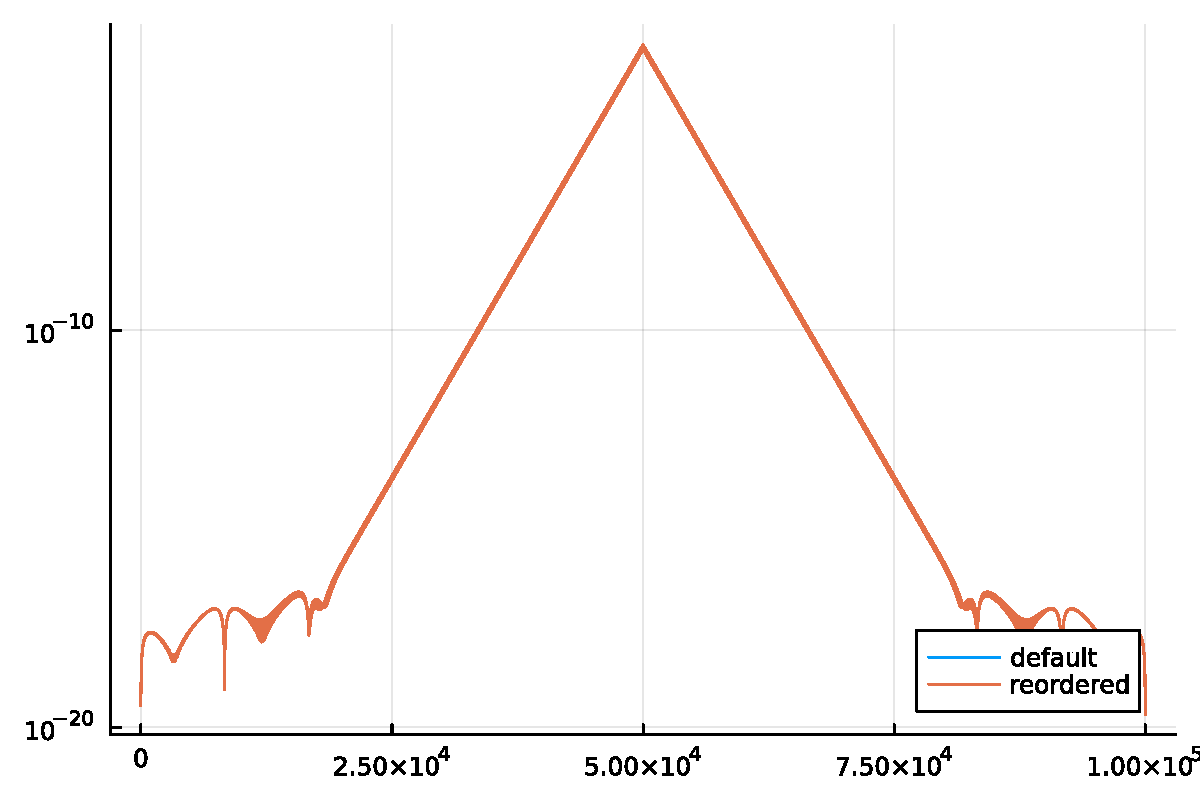
\includegraphics[width=\linewidth]{jl_fFQb2q/Fourier_7_1.pdf}

The FFT allows us to efficiently transform between "function value space"/"physical space" and "coefficient space"/"frequency space".  This is essential in the context of numerical methods for differential equations because we'll see that some operations (e.g. differentiation) can be performed much more efficiently in coefficient space than in function value space, while computing nonlinear terms may be performed more efficiently in function value space.   

\subsection{Differentiation in function value space and in coefficient space}
We have shown above that for $n$ odd with $n = 2m+1$,

\[
p(x) = \sum_{k=-m}^{m} \widetilde{c}_k{\rm e}^{{\rm i}kx},  \qquad \qquad (1)
\]
with

\[
\widetilde{c}_k = \frac{1}{n}\sum_{j=0}^{n-1}f(x_j){\rm e}^{{\rm i}kx_j}  \qquad  \qquad (2)
\]
interpolates $f$ at $x_0$, $\ldots$, $x_{n-1}$. This is a representation of the interpolant $p$ in terms of coefficients $\widetilde{c}_k$ and basis functions ${\rm e}^{{\rm i}kx}$.   Now we want to construct a different representation of $p$ in terms of function values to illustrate the difference between differentiation in function value space and coefficient space. 

Similar to the formula for the Lagrange interpolating polynomial, we want a formula for a trigonometric interpolant of the form

\[
p(x) = \sum_{j=0}^{n-1}\ell_{j}(x) f(x_{j}).
\]
Notice that now $p$ is reprented as an expansion in function values $f(x_{j})$ and basis functions $\ell_{j}(x)$. We require the basis functions to have property

\[
\ell_{j}(x_i) = \begin{cases}
1 & \text{if } i = j, i = j \pm n, i = j \pm 2n, \ldots \\
0 & \text{otherwise } 
\end{cases}
\]
so that $p(x)$ is periodic on the grid points ($p(x_{j + pn}) = p(x_{j})$, for $p \in \mathbb{Z}$) and is an interpolant ($p(x_{j}) = f(x_{j})$, for $j = 0, \ldots, n-1$). 

The idea is first to find $\ell_0(x)$ and then to set $\ell_{j}(x) = \ell_0(x-x_j)$ because then  $\ell_{j}(x_i) = \ell_0(x_{i}-x_j)$ and therefore $\ell_{j}(x_{i}) = 1$ if  $i = j$ ${\rm mod } \:n$, as required.

The function $\ell_0(x)$ can be found by using (1) and (2) to construct the interpolant of a periodic function $f$ with the property that $f(x_0) = 1$ and $f(x_j) = 0$, for $j = 1, \ldots, n-1$. For this function (a periodic, discrete delta function), the approximate Fourier coefficients are

\[
\widetilde{c}_{k} = \frac{1}{n} = \frac{h}{2\pi}, \qquad \forall k,
\]
therefore

\[
\ell_0(x) = p(x) = \sum_{k=-m}^{m} \widetilde{c}_k{\rm e}^{{\rm i}kx} = \frac{h}{2\pi}\sum_{k=-m}^{m} {\rm e}^{{\rm i}kx} = \frac{1}{n}\frac{\sin((m+1/2)x)}{\sin(x/2)}
\]
(deriving this formula is left as an exercise)

Let's check that $\ell_0(x)$ has the required properties:


\begin{lstlisting}
(*@\HLJLn{n}@*) (*@\HLJLoB{=}@*) (*@\HLJLni{11}@*)
(*@\HLJLn{m}@*) (*@\HLJLoB{=}@*) (*@\HLJLp{(}@*)(*@\HLJLn{n}@*)(*@\HLJLoB{-}@*)(*@\HLJLni{1}@*)(*@\HLJLp{)}@*)(*@\HLJLoB{\ensuremath{\div}}@*)(*@\HLJLni{2}@*)
(*@\HLJLn{h}@*) (*@\HLJLoB{=}@*) (*@\HLJLni{2}@*)(*@\HLJLn{\ensuremath{\pi}}@*)(*@\HLJLoB{/}@*)(*@\HLJLn{n}@*)
(*@\HLJLn{\ensuremath{\ell}\ensuremath{\_0}}@*) (*@\HLJLoB{=}@*) (*@\HLJLn{x}@*) (*@\HLJLoB{->}@*) (*@\HLJLn{x}@*) (*@\HLJLoB{==}@*) (*@\HLJLni{0}@*) (*@\HLJLoB{?}@*) (*@\HLJLni{1}@*) (*@\HLJLoB{:}@*) (*@\HLJLn{h}@*)(*@\HLJLoB{/}@*)(*@\HLJLp{(}@*)(*@\HLJLni{2}@*)(*@\HLJLn{\ensuremath{\pi}}@*)(*@\HLJLp{)}@*)(*@\HLJLoB{*}@*)(*@\HLJLnf{sin}@*)(*@\HLJLp{((}@*)(*@\HLJLn{m}@*)(*@\HLJLoB{+}@*)(*@\HLJLnfB{0.5}@*)(*@\HLJLp{)}@*)(*@\HLJLoB{*}@*)(*@\HLJLn{x}@*)(*@\HLJLp{)}@*)(*@\HLJLoB{/}@*)(*@\HLJLnf{sin}@*)(*@\HLJLp{(}@*)(*@\HLJLn{x}@*)(*@\HLJLoB{/}@*)(*@\HLJLni{2}@*)(*@\HLJLp{)}@*)
(*@\HLJLn{x}@*) (*@\HLJLoB{=}@*) (*@\HLJLnf{range}@*)(*@\HLJLp{(}@*)(*@\HLJLni{0}@*)(*@\HLJLp{,}@*)(*@\HLJLni{2}@*)(*@\HLJLn{\ensuremath{\pi}}@*)(*@\HLJLp{;}@*)(*@\HLJLn{length}@*)(*@\HLJLoB{=}@*)(*@\HLJLn{n}@*)(*@\HLJLoB{+}@*)(*@\HLJLni{1}@*)(*@\HLJLp{)[}@*)(*@\HLJLni{1}@*)(*@\HLJLoB{:}@*)(*@\HLJLk{end}@*)(*@\HLJLoB{-}@*)(*@\HLJLni{1}@*)(*@\HLJLp{]}@*) (*@\HLJLcs{{\#}x\ensuremath{\_0},}@*) (*@\HLJLcs{\ensuremath{\ldots},}@*) (*@\HLJLcs{x{\_}{\{}n-1{\}}}@*)
(*@\HLJLn{xx}@*) (*@\HLJLoB{=}@*) (*@\HLJLnf{range}@*)(*@\HLJLp{(}@*)(*@\HLJLni{0}@*)(*@\HLJLp{,}@*)(*@\HLJLni{2}@*)(*@\HLJLn{\ensuremath{\pi}}@*)(*@\HLJLp{;}@*)(*@\HLJLn{length}@*)(*@\HLJLoB{=}@*)(*@\HLJLni{501}@*)(*@\HLJLp{)[}@*)(*@\HLJLni{1}@*)(*@\HLJLoB{:}@*)(*@\HLJLk{end}@*)(*@\HLJLoB{-}@*)(*@\HLJLni{1}@*)(*@\HLJLp{]}@*) (*@\HLJLcs{{\#}plotting}@*) (*@\HLJLcs{grid}@*)
(*@\HLJLnf{plot}@*)(*@\HLJLp{(}@*)(*@\HLJLn{xx}@*)(*@\HLJLp{,}@*)(*@\HLJLn{\ensuremath{\ell}\ensuremath{\_0}}@*)(*@\HLJLoB{.}@*)(*@\HLJLp{(}@*)(*@\HLJLn{xx}@*)(*@\HLJLp{);}@*)(*@\HLJLn{label}@*)(*@\HLJLoB{=}@*)(*@\HLJLs{"{}\ensuremath{\ell}\ensuremath{\_0}(x)"{}}@*)(*@\HLJLp{)}@*)
(*@\HLJLnf{scatter!}@*)(*@\HLJLp{(}@*)(*@\HLJLn{x}@*)(*@\HLJLp{,}@*)(*@\HLJLn{\ensuremath{\ell}\ensuremath{\_0}}@*)(*@\HLJLoB{.}@*)(*@\HLJLp{(}@*)(*@\HLJLn{x}@*)(*@\HLJLp{);}@*)(*@\HLJLn{label}@*)(*@\HLJLoB{=}@*)(*@\HLJLs{"{}samples"{}}@*)(*@\HLJLp{)}@*)
\end{lstlisting}

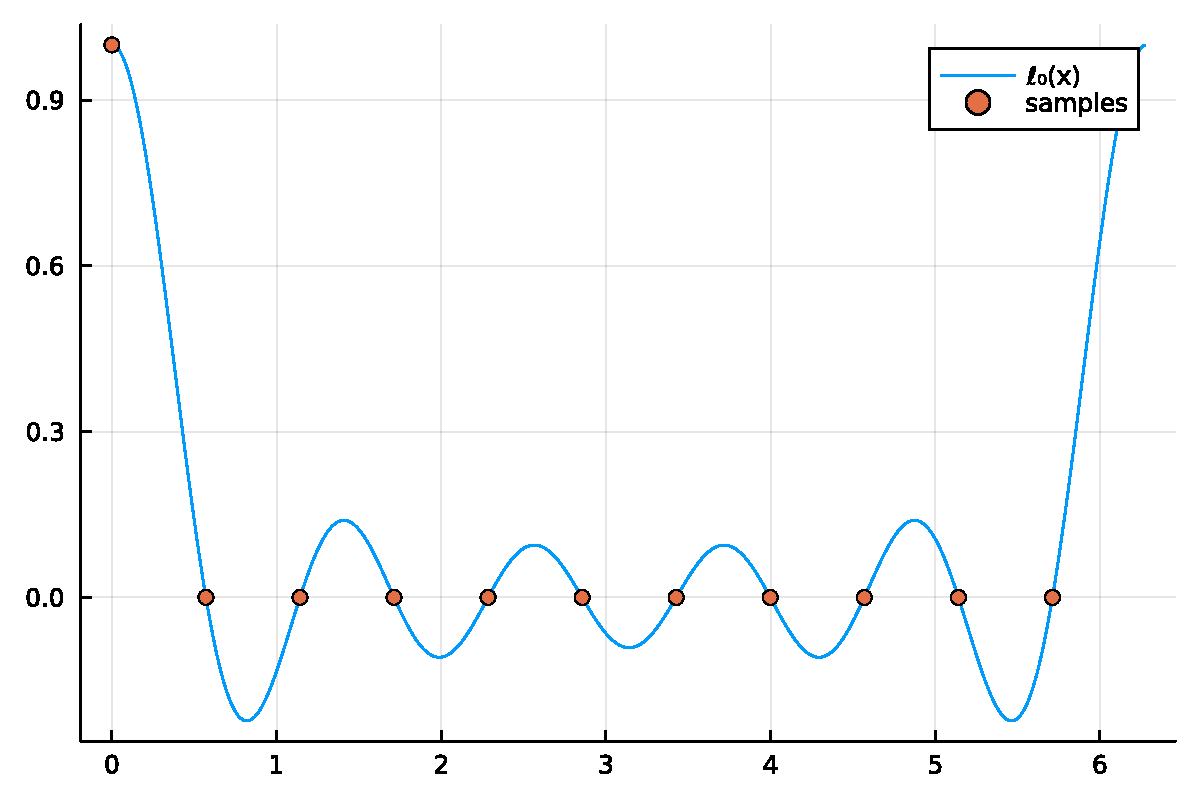
\includegraphics[width=\linewidth]{jl_fFQb2q/Fourier_8_1.pdf}

Here is a translated version of $\ell_0(x)$, namely $\ell_0(x-x_{m}) = \ell_{m}(x)$


\begin{lstlisting}
(*@\HLJLnf{plot}@*)(*@\HLJLp{(}@*)(*@\HLJLn{xx}@*)(*@\HLJLp{,}@*)(*@\HLJLn{\ensuremath{\ell}\ensuremath{\_0}}@*)(*@\HLJLoB{.}@*)(*@\HLJLp{(}@*)(*@\HLJLn{xx}@*) (*@\HLJLoB{.-}@*) (*@\HLJLn{x}@*)(*@\HLJLp{[}@*)(*@\HLJLn{m}@*)(*@\HLJLoB{+}@*)(*@\HLJLni{1}@*)(*@\HLJLp{]);}@*)(*@\HLJLn{label}@*)(*@\HLJLoB{=}@*)(*@\HLJLs{"{}\ensuremath{\ell}\ensuremath{\_m}(x)"{}}@*)(*@\HLJLp{)}@*)
(*@\HLJLnf{scatter!}@*)(*@\HLJLp{(}@*)(*@\HLJLn{x}@*)(*@\HLJLp{,}@*)(*@\HLJLn{\ensuremath{\ell}\ensuremath{\_0}}@*)(*@\HLJLoB{.}@*)(*@\HLJLp{(}@*)(*@\HLJLn{x}@*) (*@\HLJLoB{.-}@*) (*@\HLJLn{x}@*)(*@\HLJLp{[}@*)(*@\HLJLn{m}@*)(*@\HLJLoB{+}@*)(*@\HLJLni{1}@*)(*@\HLJLp{]);}@*)(*@\HLJLn{label}@*)(*@\HLJLoB{=}@*)(*@\HLJLs{"{}samples"{}}@*)(*@\HLJLp{)}@*)
\end{lstlisting}

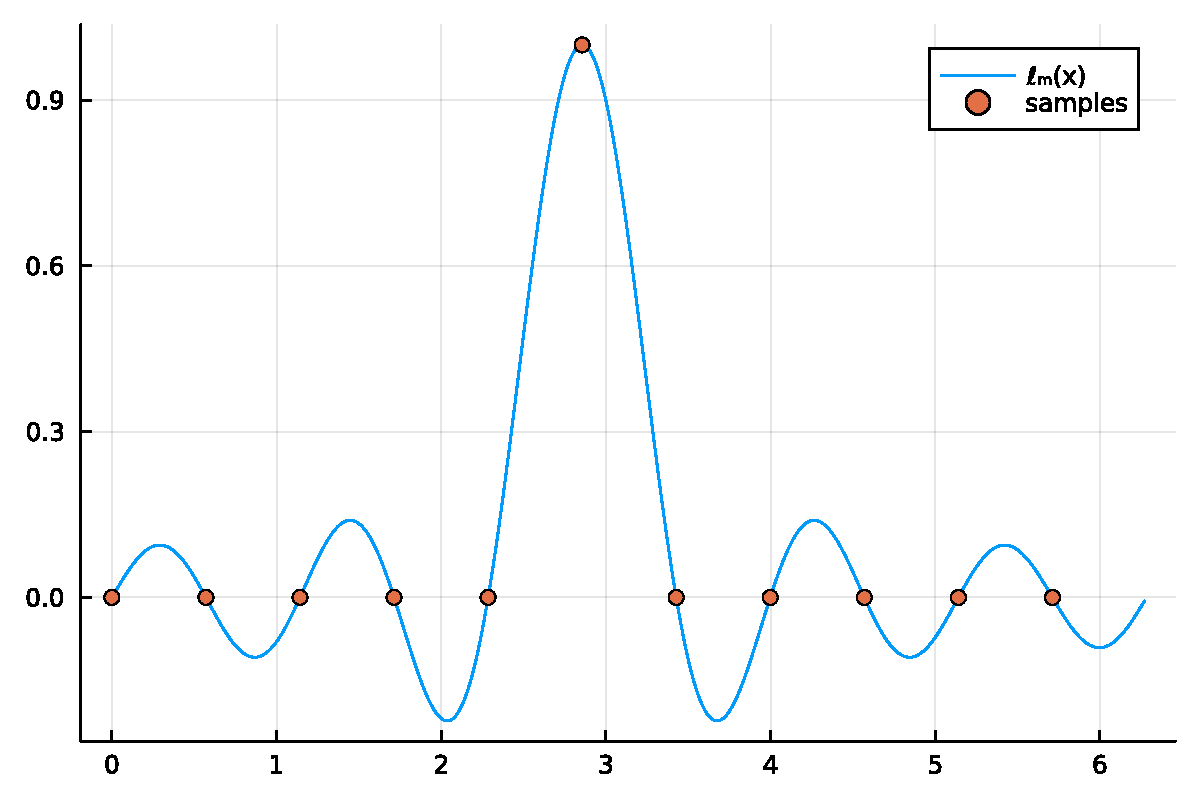
\includegraphics[width=\linewidth]{jl_fFQb2q/Fourier_9_1.pdf}

Hence, another representation of the interpolant is

\[
p(x) = \sum_{j=0}^{n-1}\ell_j(x)f(x_j) = \sum_{j=0}^{n-1}\ell_0(x-x_j)f(x_j), \qquad \ell_0(x) = \frac{1}{n}\frac{\sin((m+1/2)x)}{\sin(x/2)}
\]
from which we obtain approximations to the derivative at the grid points $x_j$, $j = 0, \ldots, n-1$:

\[
f'(x_i) \approx p'(x_i) = \sum_{j=0}^{n-1}\ell_{j}'(x_i) f(x_{j})  = \sum_{j=0}^{n-1}\ell_{0}'(x_i-x_j)f(x_{j}), \qquad i = 0, \ldots, n-1.
\]
It is left as an exercise to show that

\[
\ell_{0}'(x_i-x_j) = \begin{cases}
 0 & \text{if } i = j \\
 \frac{(-1)^{i-j}}{2}\csc\left( \frac{(i-j)h}{2} \right)  & \text{if } i\neq j
\end{cases}.
\]
This implies that the differentiation matrix is Toeplitz and the entries on the $(i-j)$-th diagonal is $\frac{(-1)^{i-j}}{2}\csc\left( \frac{(i-j)h}{2} \right)$, i.e.,

\[
\left(
\begin{array}{c}
f'(x_0) \\
  \\
\vdots  \\
  \\
f'(x_{n-1})
\end{array}
\right) \approx 
\left(
\begin{array}{c}
p'(x_0) \\
  \\
\vdots  \\
  \\
p'(x_{n-1})
\end{array}
\right) = 
\left(
\begin{array}{c c c c c c c}
  &       &       & \vdots  &   &   & \\
  &\ddots &       & \frac{1}{2}\csc \frac{3h}{2}   &   &    &  \\
   &\ddots &      &-\frac{1}{2}\csc \frac{2h}{2}   &   &    &  \\ 
   &\ddots &      & \frac{1}{2}\csc \frac{1h}{2}   &   &    &   \\
  &        &      & 0                              &   &    &   \\
&      &      & -\frac{1}{2}\csc \frac{1h}{2}   &   &   \ddots &  \\
&      &      & \frac{1}{2}\csc \frac{2h}{2}   &   &   \ddots &  \\
&      &      & -\frac{1}{2}\csc \frac{3h}{2}   &   &   \ddots &  \\
&      &      & \vdots  &   &    &  \\
\end{array}
\right)
\left(
\begin{array}{c}
f_0 \\
  \\
\vdots  \\
  \\
f_{n-1}
\end{array}
\right).
\]
Alternatively, we can approximate $f'$ by differentiating the "coefficient space" interpolant (1):

\[
f'(x) \approx p'(x) = \sum_{k=-m}^{m} {\rm i k}\widetilde{c}_k{\rm e}^{{\rm i}kx}.
\]
Similarly, we approximate the $\nu$-th order derivative with $\nu \in \mathbb{Z}_+$ as

\[
f^{(\nu)}(x) \approx p^{(\nu)}(x) = \sum_{k=-m}^{m} \left({\rm i k}\right)^{\nu}\,\widetilde{c}_k{\rm e}^{{\rm i}kx}.
\]
Let's denote the Fourier coefficients of $f^{(\nu)}(x)$ by $c_k^{(\nu)}$, then

\[
f^{(\nu)}(x) = \sum_{k=-\infty}^{\infty}c_k^{(\nu)}{\rm e}^{{\rm i}kx},
\]
where $c_k^{(\nu)} =  \left( {\rm i}k \right)^{\nu} c_k$.  Therefore we approximate $c_k^{(\nu)}$ using the Fourier coefficients of $p^{(\nu)}(x)$, i.e.,

\[
\left(
\begin{array}{c}
c_{-m}^{(\nu)} \\
\vdots \\
c_{m}^{(\nu)}
\end{array}
\right) \approx
\left(
\begin{array}{c c c}
\left(-{\rm i}m\right)^{\nu} &  &   \\
   & \ddots &    \\
   &        & \left({\rm i}m\right)^{\nu}
\end{array}
\right)
\left(
\begin{array}{c}
\widetilde{c}_{-m} \\
\vdots \\
\widetilde{c}_{m}
\end{array}
\right).
\]
Note that in "coefficient space", the differentiation matrix is diagonal whereas it is dense in "function value" space.  

Starting from the function values on the grid, $f(x_j)$, $j = 0, \ldots, n-1$, we can approximate $f^{(\nu)}(x_j) \approx p^{(\nu)}(x_j)$, $j = 0, \ldots, n-1$ using the FFT and inverse FFT as follows:

\begin{itemize}
\item[1. ] compute $\tilde{c}_{-m}, \ldots, \tilde{c}_{m}$ using the FFT  (function values to coefficients)


\item[2. ] compute $(-{\rm i}m)^{\nu}\,\tilde{c}_{-m}, (-{\rm i}(m-1))^{\nu}\,\tilde{c}_{-(m-1)}, \ldots, ({\rm i}m)^{\nu}\,\tilde{c}_{m}$ (differentiate in coefficient space)


\item[3. ] compute $p^{(\nu)}(x_j)$ using the (inverse) FFT  (coefficients to function values)

\end{itemize}
Note that this procedure has $\mathcal{O}(n \log n)$ complexity where naive multiplication by a dense differentiation matrix has quadratic complexity ($\mathcal{O}\left(n^2\right)$).

Here is an example:


\begin{lstlisting}
(*@\HLJLn{f}@*) (*@\HLJLoB{=}@*) (*@\HLJLn{x}@*) (*@\HLJLoB{->}@*) (*@\HLJLni{1}@*)(*@\HLJLoB{/}@*)(*@\HLJLp{(}@*)(*@\HLJLni{2}@*) (*@\HLJLoB{+}@*) (*@\HLJLnf{cos}@*)(*@\HLJLp{(}@*)(*@\HLJLn{x}@*)(*@\HLJLp{))}@*)
(*@\HLJLn{Df}@*) (*@\HLJLoB{=}@*) (*@\HLJLn{x}@*) (*@\HLJLoB{->}@*) (*@\HLJLnf{sin}@*)(*@\HLJLp{(}@*)(*@\HLJLn{x}@*)(*@\HLJLp{)}@*)(*@\HLJLoB{/}@*)(*@\HLJLp{(}@*)(*@\HLJLni{2}@*) (*@\HLJLoB{+}@*) (*@\HLJLnf{cos}@*)(*@\HLJLp{(}@*)(*@\HLJLn{x}@*)(*@\HLJLp{))}@*)(*@\HLJLoB{{\textasciicircum}}@*)(*@\HLJLni{2}@*)  (*@\HLJLcs{{\#}}@*) (*@\HLJLcs{derivative}@*)
(*@\HLJLn{n}@*) (*@\HLJLoB{=}@*) (*@\HLJLni{101}@*)
(*@\HLJLn{m}@*) (*@\HLJLoB{=}@*) (*@\HLJLp{(}@*)(*@\HLJLn{n}@*)(*@\HLJLoB{-}@*)(*@\HLJLni{1}@*)(*@\HLJLp{)}@*)(*@\HLJLoB{\ensuremath{\div}}@*)(*@\HLJLni{2}@*)
(*@\HLJLn{x}@*) (*@\HLJLoB{=}@*) (*@\HLJLnf{range}@*)(*@\HLJLp{(}@*)(*@\HLJLni{0}@*)(*@\HLJLp{,}@*)(*@\HLJLni{2}@*)(*@\HLJLn{\ensuremath{\pi}}@*)(*@\HLJLp{;}@*)(*@\HLJLn{length}@*)(*@\HLJLoB{=}@*)(*@\HLJLn{n}@*)(*@\HLJLoB{+}@*)(*@\HLJLni{1}@*)(*@\HLJLp{)[}@*)(*@\HLJLni{1}@*)(*@\HLJLoB{:}@*)(*@\HLJLk{end}@*)(*@\HLJLoB{-}@*)(*@\HLJLni{1}@*)(*@\HLJLp{]}@*) (*@\HLJLcs{{\#}}@*) (*@\HLJLcs{grid}@*) (*@\HLJLcs{points}@*) (*@\HLJLcs{x\ensuremath{\_0},}@*) (*@\HLJLcs{\ensuremath{\ldots},}@*) (*@\HLJLcs{x\ensuremath{\_n}\ensuremath{\_-}\ensuremath{\_1}}@*)
(*@\HLJLcs{{\#}}@*) (*@\HLJLcs{map}@*) (*@\HLJLcs{function}@*) (*@\HLJLcs{values}@*) (*@\HLJLcs{to}@*) (*@\HLJLcs{coefficients}@*) (*@\HLJLcs{via}@*) (*@\HLJLcs{the}@*) (*@\HLJLcs{fft}@*)
(*@\HLJLn{c}@*) (*@\HLJLoB{=}@*) (*@\HLJLnf{fft}@*)(*@\HLJLp{(}@*)(*@\HLJLn{f}@*)(*@\HLJLoB{.}@*)(*@\HLJLp{(}@*)(*@\HLJLn{x}@*)(*@\HLJLp{))}@*)(*@\HLJLoB{/}@*)(*@\HLJLn{n}@*)(*@\HLJLp{;}@*) (*@\HLJLcs{{\#}}@*) (*@\HLJLcs{[c\ensuremath{\_0},}@*) (*@\HLJLcs{\ensuremath{\ldots},}@*) (*@\HLJLcs{c\ensuremath{\_n}\ensuremath{\_-}\ensuremath{\_1}]}@*)
(*@\HLJLcs{{\#}}@*) (*@\HLJLcs{re-order}@*) (*@\HLJLcs{coefficients}@*)
(*@\HLJLn{ch}@*) (*@\HLJLoB{=}@*) (*@\HLJLnf{fftshift}@*)(*@\HLJLp{(}@*)(*@\HLJLn{c}@*)(*@\HLJLp{);}@*)  (*@\HLJLcs{{\#}}@*) (*@\HLJLcs{reorder}@*) (*@\HLJLcs{the}@*) (*@\HLJLcs{coefficients}@*) (*@\HLJLcs{to}@*) (*@\HLJLcs{[c\ensuremath{\_-}\ensuremath{\_m},}@*) (*@\HLJLcs{\ensuremath{\ldots},}@*) (*@\HLJLcs{c\ensuremath{\_m}]}@*)
(*@\HLJLcs{{\#}}@*) (*@\HLJLcs{Fourier}@*) (*@\HLJLcs{coefficients}@*) (*@\HLJLcs{of}@*) (*@\HLJLcs{the}@*) (*@\HLJLcs{derivative}@*)
(*@\HLJLn{dch}@*) (*@\HLJLoB{=}@*) (*@\HLJLp{(}@*)(*@\HLJLn{im}@*)(*@\HLJLoB{*}@*)(*@\HLJLp{(}@*)(*@\HLJLoB{-}@*)(*@\HLJLn{m}@*)(*@\HLJLoB{:}@*)(*@\HLJLn{m}@*)(*@\HLJLp{))}@*)(*@\HLJLoB{.*}@*)(*@\HLJLn{ch}@*)(*@\HLJLp{;}@*)
(*@\HLJLcs{{\#}}@*) (*@\HLJLcs{re-order}@*)
(*@\HLJLn{dc}@*) (*@\HLJLoB{=}@*) (*@\HLJLnf{ifftshift}@*)(*@\HLJLp{(}@*)(*@\HLJLn{dch}@*)(*@\HLJLp{);}@*) (*@\HLJLcs{{\#}}@*) (*@\HLJLcs{undoes}@*) (*@\HLJLcs{what}@*) (*@\HLJLcs{fftshift}@*) (*@\HLJLcs{did}@*)
(*@\HLJLcs{{\#}}@*) (*@\HLJLcs{map}@*) (*@\HLJLcs{coefficients}@*) (*@\HLJLcs{to}@*) (*@\HLJLcs{function}@*) (*@\HLJLcs{values}@*) (*@\HLJLcs{via}@*) (*@\HLJLcs{the}@*) (*@\HLJLcs{ifft}@*)
(*@\HLJLn{df}@*) (*@\HLJLoB{=}@*) (*@\HLJLn{n}@*)(*@\HLJLoB{*}@*)(*@\HLJLnf{ifft}@*)(*@\HLJLp{(}@*)(*@\HLJLn{dc}@*)(*@\HLJLp{);}@*)
(*@\HLJLnf{norm}@*)(*@\HLJLp{(}@*)(*@\HLJLn{df}@*) (*@\HLJLoB{-}@*) (*@\HLJLn{Df}@*)(*@\HLJLoB{.}@*)(*@\HLJLp{(}@*)(*@\HLJLn{x}@*)(*@\HLJLp{),}@*)(*@\HLJLn{Inf}@*)(*@\HLJLp{)}@*)
\end{lstlisting}

\begin{lstlisting}
1.7790211156964822e-14
\end{lstlisting}


\begin{lstlisting}
(*@\HLJLcs{{\#}}@*) (*@\HLJLcs{more}@*) (*@\HLJLcs{briefly}@*)
(*@\HLJLn{df}@*) (*@\HLJLoB{=}@*) (*@\HLJLnf{ifft}@*)(*@\HLJLp{(}@*)(*@\HLJLnf{ifftshift}@*)(*@\HLJLp{(}@*)(*@\HLJLn{im}@*)(*@\HLJLoB{*}@*)(*@\HLJLp{(}@*)(*@\HLJLoB{-}@*)(*@\HLJLn{m}@*)(*@\HLJLoB{:}@*)(*@\HLJLn{m}@*)(*@\HLJLp{))}@*)(*@\HLJLoB{.*}@*)(*@\HLJLnf{fft}@*)(*@\HLJLp{(}@*)(*@\HLJLn{f}@*)(*@\HLJLoB{.}@*)(*@\HLJLp{(}@*)(*@\HLJLn{x}@*)(*@\HLJLp{)))}@*)
(*@\HLJLnf{norm}@*)(*@\HLJLp{(}@*)(*@\HLJLn{df}@*) (*@\HLJLoB{-}@*) (*@\HLJLn{Df}@*)(*@\HLJLoB{.}@*)(*@\HLJLp{(}@*)(*@\HLJLn{x}@*)(*@\HLJLp{),}@*)(*@\HLJLn{Inf}@*)(*@\HLJLp{)}@*)
\end{lstlisting}

\begin{lstlisting}
1.7726178619566572e-14
\end{lstlisting}


Mathematically, we express approximate $\nu$-th order differentation of a function $f(x)$ on the equispaced grid $x_j = jh = 2\pi j/n$, $j = 0, \ldots, n-1$ with $n = 2m + 1$ as follows

\[
\mathcal{F}^{-1}\left\lbrace\left({\rm i}(-m\!:\!m)\right)^{\nu}\cdot\mathcal{F}\lbrace \mathbf{f} \rbrace\right\rbrace
\]
Here we approximate $f'(x_j)$, $j = 0, \ldots, n-1$ using (i) differentiation matrices and (ii) the FFT.


\begin{lstlisting}
(*@\HLJLk{using}@*) (*@\HLJLn{ToeplitzMatrices}@*)
(*@\HLJLn{nv}@*) (*@\HLJLoB{=}@*) (*@\HLJLni{5}@*)(*@\HLJLoB{:}@*)(*@\HLJLni{2}@*)(*@\HLJLoB{:}@*)(*@\HLJLni{71}@*)
(*@\HLJLn{f}@*) (*@\HLJLoB{=}@*) (*@\HLJLn{x}@*) (*@\HLJLoB{->}@*) (*@\HLJLni{1}@*)(*@\HLJLoB{/}@*)(*@\HLJLp{(}@*)(*@\HLJLni{2}@*) (*@\HLJLoB{+}@*) (*@\HLJLnf{cos}@*)(*@\HLJLp{(}@*)(*@\HLJLn{x}@*)(*@\HLJLp{))}@*)
(*@\HLJLn{Df}@*) (*@\HLJLoB{=}@*) (*@\HLJLn{x}@*) (*@\HLJLoB{->}@*) (*@\HLJLnf{sin}@*)(*@\HLJLp{(}@*)(*@\HLJLn{x}@*)(*@\HLJLp{)}@*)(*@\HLJLoB{/}@*)(*@\HLJLp{(}@*)(*@\HLJLni{2}@*) (*@\HLJLoB{+}@*) (*@\HLJLnf{cos}@*)(*@\HLJLp{(}@*)(*@\HLJLn{x}@*)(*@\HLJLp{))}@*)(*@\HLJLoB{{\textasciicircum}}@*)(*@\HLJLni{2}@*)  (*@\HLJLcs{{\#}}@*) (*@\HLJLcs{derivative}@*)

(*@\HLJLcs{{\#}}@*) (*@\HLJLcs{Differentiation}@*) (*@\HLJLcs{matrices}@*)
(*@\HLJLn{errs}@*) (*@\HLJLoB{=}@*) 
(*@\HLJLp{[(}@*) (*@\HLJLn{h}@*) (*@\HLJLoB{=}@*) (*@\HLJLni{2}@*)(*@\HLJLn{\ensuremath{\pi}}@*)(*@\HLJLoB{/}@*)(*@\HLJLn{n}@*)(*@\HLJLp{;}@*)
    (*@\HLJLn{column}@*) (*@\HLJLoB{=}@*) (*@\HLJLp{[}@*)(*@\HLJLni{0}@*)(*@\HLJLp{;}@*) (*@\HLJLnfB{0.5}@*)(*@\HLJLoB{*}@*)(*@\HLJLp{(}@*)(*@\HLJLoB{-}@*)(*@\HLJLni{1}@*)(*@\HLJLp{)}@*)(*@\HLJLoB{.{\textasciicircum}}@*)(*@\HLJLp{(}@*)(*@\HLJLni{1}@*)(*@\HLJLoB{:}@*)(*@\HLJLn{n}@*)(*@\HLJLoB{-}@*)(*@\HLJLni{1}@*)(*@\HLJLp{)}@*)(*@\HLJLoB{.*}@*)(*@\HLJLn{csc}@*)(*@\HLJLoB{.}@*)(*@\HLJLp{((}@*)(*@\HLJLni{1}@*)(*@\HLJLoB{:}@*)(*@\HLJLn{n}@*)(*@\HLJLoB{-}@*)(*@\HLJLni{1}@*)(*@\HLJLp{)}@*)(*@\HLJLoB{*}@*)(*@\HLJLn{h}@*)(*@\HLJLoB{/}@*)(*@\HLJLni{2}@*)(*@\HLJLp{)];}@*)
    (*@\HLJLn{D\ensuremath{\_n}}@*) (*@\HLJLoB{=}@*) (*@\HLJLnf{Toeplitz}@*)(*@\HLJLp{(}@*)(*@\HLJLn{column}@*)(*@\HLJLp{,[}@*)(*@\HLJLn{column}@*)(*@\HLJLp{[}@*)(*@\HLJLni{1}@*)(*@\HLJLp{];}@*) (*@\HLJLn{column}@*)(*@\HLJLp{[}@*)(*@\HLJLn{n}@*)(*@\HLJLoB{:-}@*)(*@\HLJLni{1}@*)(*@\HLJLoB{:}@*)(*@\HLJLni{2}@*)(*@\HLJLp{]]);}@*) (*@\HLJLcs{{\#}}@*) (*@\HLJLcs{Differentiation}@*) (*@\HLJLcs{matrix:}@*)
    (*@\HLJLn{x}@*) (*@\HLJLoB{=}@*) (*@\HLJLnf{range}@*)(*@\HLJLp{(}@*)(*@\HLJLni{0}@*)(*@\HLJLp{,}@*)(*@\HLJLni{2}@*)(*@\HLJLn{\ensuremath{\pi}}@*)(*@\HLJLp{;}@*)(*@\HLJLn{length}@*)(*@\HLJLoB{=}@*)(*@\HLJLn{n}@*)(*@\HLJLoB{+}@*)(*@\HLJLni{1}@*)(*@\HLJLp{)[}@*)(*@\HLJLni{1}@*)(*@\HLJLoB{:}@*)(*@\HLJLk{end}@*)(*@\HLJLoB{-}@*)(*@\HLJLni{1}@*)(*@\HLJLp{];}@*) (*@\HLJLcs{{\#}}@*) (*@\HLJLcs{n}@*) (*@\HLJLcs{equally}@*) (*@\HLJLcs{spaced}@*) (*@\HLJLcs{points}@*) (*@\HLJLcs{on}@*) (*@\HLJLcs{[0,}@*) (*@\HLJLcs{2\ensuremath{\pi})}@*)
    (*@\HLJLnf{norm}@*)(*@\HLJLp{(}@*)(*@\HLJLn{D\ensuremath{\_n}}@*)(*@\HLJLoB{*}@*)(*@\HLJLn{f}@*)(*@\HLJLoB{.}@*)(*@\HLJLp{(}@*)(*@\HLJLn{x}@*)(*@\HLJLp{)}@*) (*@\HLJLoB{-}@*) (*@\HLJLn{Df}@*)(*@\HLJLoB{.}@*)(*@\HLJLp{(}@*)(*@\HLJLn{x}@*)(*@\HLJLp{),}@*)(*@\HLJLn{Inf}@*)(*@\HLJLp{)}@*) (*@\HLJLp{)}@*) (*@\HLJLk{for}@*) (*@\HLJLn{n}@*) (*@\HLJLoB{=}@*) (*@\HLJLn{nv}@*)(*@\HLJLp{]}@*) (*@\HLJLcs{{\#}}@*) (*@\HLJLcs{maximum}@*) (*@\HLJLcs{error}@*) (*@\HLJLcs{at}@*) (*@\HLJLcs{the}@*) (*@\HLJLcs{set}@*) (*@\HLJLcs{of}@*) (*@\HLJLcs{N}@*) (*@\HLJLcs{points}@*)

(*@\HLJLcs{{\#}}@*) (*@\HLJLcs{Differentiation}@*) (*@\HLJLcs{in}@*) (*@\HLJLcs{coefficient}@*) (*@\HLJLcs{space}@*) (*@\HLJLcs{via}@*) (*@\HLJLcs{the}@*) (*@\HLJLcs{FFT}@*)
(*@\HLJLn{errsfft}@*) (*@\HLJLoB{=}@*) 
(*@\HLJLp{[(}@*)  (*@\HLJLn{m}@*) (*@\HLJLoB{=}@*) (*@\HLJLp{(}@*)(*@\HLJLn{n}@*)(*@\HLJLoB{-}@*)(*@\HLJLni{1}@*)(*@\HLJLp{)}@*)(*@\HLJLoB{\ensuremath{\div}}@*)(*@\HLJLni{2}@*)(*@\HLJLp{;}@*)
    (*@\HLJLn{x}@*) (*@\HLJLoB{=}@*) (*@\HLJLnf{range}@*)(*@\HLJLp{(}@*)(*@\HLJLni{0}@*)(*@\HLJLp{,}@*)(*@\HLJLni{2}@*)(*@\HLJLn{\ensuremath{\pi}}@*)(*@\HLJLp{;}@*)(*@\HLJLn{length}@*)(*@\HLJLoB{=}@*)(*@\HLJLn{n}@*)(*@\HLJLoB{+}@*)(*@\HLJLni{1}@*)(*@\HLJLp{)[}@*)(*@\HLJLni{1}@*)(*@\HLJLoB{:}@*)(*@\HLJLk{end}@*)(*@\HLJLoB{-}@*)(*@\HLJLni{1}@*)(*@\HLJLp{];}@*)
    (*@\HLJLn{df}@*) (*@\HLJLoB{=}@*) (*@\HLJLnf{ifft}@*)(*@\HLJLp{(}@*)(*@\HLJLnf{ifftshift}@*)(*@\HLJLp{(}@*)(*@\HLJLn{im}@*)(*@\HLJLoB{*}@*)(*@\HLJLp{(}@*)(*@\HLJLoB{-}@*)(*@\HLJLn{m}@*)(*@\HLJLoB{:}@*)(*@\HLJLn{m}@*)(*@\HLJLp{))}@*)(*@\HLJLoB{.*}@*)(*@\HLJLnf{fft}@*)(*@\HLJLp{(}@*)(*@\HLJLn{f}@*)(*@\HLJLoB{.}@*)(*@\HLJLp{(}@*)(*@\HLJLn{x}@*)(*@\HLJLp{)));}@*)
    (*@\HLJLnf{norm}@*)(*@\HLJLp{(}@*)(*@\HLJLn{df}@*) (*@\HLJLoB{-}@*) (*@\HLJLn{Df}@*)(*@\HLJLoB{.}@*)(*@\HLJLp{(}@*)(*@\HLJLn{x}@*)(*@\HLJLp{),}@*)(*@\HLJLn{Inf}@*)(*@\HLJLp{)}@*) (*@\HLJLp{)}@*) (*@\HLJLk{for}@*) (*@\HLJLn{n}@*) (*@\HLJLoB{=}@*) (*@\HLJLn{nv}@*)(*@\HLJLp{]}@*)

(*@\HLJLcs{{\#}}@*) (*@\HLJLcs{plot}@*) (*@\HLJLcs{the}@*) (*@\HLJLcs{error}@*) (*@\HLJLcs{on}@*) (*@\HLJLcs{a}@*) (*@\HLJLcs{semi-log}@*) (*@\HLJLcs{(log-linear)}@*) (*@\HLJLcs{scale}@*)
(*@\HLJLnf{scatter}@*)(*@\HLJLp{(}@*)(*@\HLJLn{nv}@*)(*@\HLJLp{,}@*)(*@\HLJLn{errs}@*)(*@\HLJLp{;}@*)(*@\HLJLn{yscale}@*)(*@\HLJLoB{=:}@*)(*@\HLJLn{log10}@*)(*@\HLJLp{,}@*)(*@\HLJLn{ms}@*)(*@\HLJLoB{=}@*)(*@\HLJLni{7}@*)(*@\HLJLp{,}@*)(*@\HLJLn{label}@*)(*@\HLJLoB{=}@*)(*@\HLJLs{"{}Error:}@*) (*@\HLJLs{differentiation}@*) (*@\HLJLs{matrix"{}}@*)(*@\HLJLp{)}@*)
(*@\HLJLnf{scatter!}@*)(*@\HLJLp{(}@*)(*@\HLJLn{nv}@*)(*@\HLJLp{,}@*)(*@\HLJLn{errsfft}@*)(*@\HLJLp{;}@*)(*@\HLJLn{yscale}@*)(*@\HLJLoB{=:}@*)(*@\HLJLn{log10}@*)(*@\HLJLp{,}@*)(*@\HLJLn{label}@*)(*@\HLJLoB{=}@*)(*@\HLJLs{"{}Error:}@*) (*@\HLJLs{differentiation}@*) (*@\HLJLs{via}@*) (*@\HLJLs{FFT"{}}@*)(*@\HLJLp{)}@*)
\end{lstlisting}

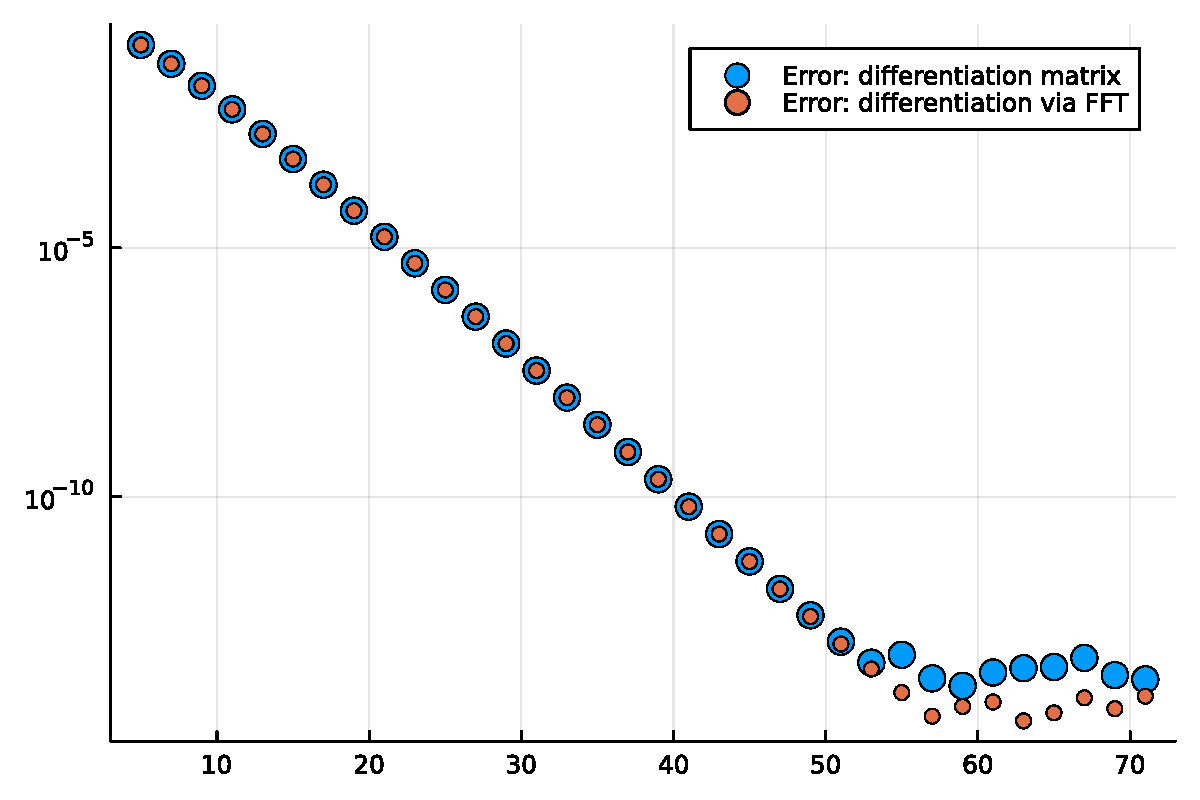
\includegraphics[width=\linewidth]{jl_fFQb2q/Fourier_12_1.pdf}

\subsection{PDE example}
Now we have the tools to implement a numerical method for the \emph{advection equation}

\[
u_t + u_x = 0, \qquad u = u(x,t).
\]
We want to approximate the solution to this equation with the initial data

\[
u(x,0) = f(x) = {\rm e}^{-100(x-1)^2}.
\]
We can easily verify that the exact solution to this Cauchy problem is

\[
u(x,t) = f(x - t).
\]
This solution can be derived using the method of characteristics.     

As it stands, this problem is posed on the entire real real line.  However, since the initial data decay very rapdily to zero away from $x=1$, it is approximately periodic on $[0, 2\pi]$ and therefore we approximate $u(x,t)$ in the $x$-direction using Fourier methods. 

We let the equispaced spatial grid be

\[
x_j = jh = j \frac{2\pi}{n_x}, \qquad j = 0, \ldots, n_x-1, \qquad n_x = 2m+1
\]
and we let $t \in [0, T]$ and set

\[
t_i = i\tau, \qquad \tau = \frac{T}{n_t}, \qquad i = 0, \ldots, n_t.
\]
We let $u^{i}_j$ denote the approximation to the exact solution $u$ at $x=x_j$ and $t = t_i$, i.e.,

\[
u^{i}_j \approx u(x_j, t_i).
\]
(the index $i$ should not be confused with the imaginary unit ${\rm i} = \sqrt{-1}$).  We set $u^{0}_j = u(x_j,0) = f(x_j)$ or, in vector notation, $\mathbf{u}^{0} = \mathbf{f}$.

We approximate the time-derivative with forward differences:

\[
u_t(x_j,t_i) \approx \frac{u(x_j,t_{i+1}) - u(x_j,t_{i})}{\tau} \approx \frac{u^{i+1}_j - u^{i}_j}{\tau}, \qquad j = 0, \ldots, n_x-1
\]
or, in vector notation,

\[
u_t(\mathbf{x},t_i) \approx \frac{\mathbf{u}^{i+1} - \mathbf{u}^{i}}{\tau}.
\]
We approximate the spatial derivative using the FFT!:

\[
u_x(\mathbf{x},t_i) \approx \mathcal{F}^{-1}\left\lbrace {\rm i}(-m\!:\!m)\cdot\mathcal{F}\lbrace \mathbf{u}^{i} \rbrace\right\rbrace
\]
Therefore we approximate the solution to the PDE as follows:

\[
\mathbf{u}^{i+1} = \mathbf{u}^{i} - \tau \mathcal{F}^{-1}\left\lbrace {\rm i}(-m\!:\!m)\cdot\mathcal{F}\lbrace \mathbf{u}^{i} \rbrace\right\rbrace, \qquad i = 0, \ldots, n_t-1, \qquad \mathbf{u}^0 = \mathbf{f}.
\]

\begin{lstlisting}
(*@\HLJLn{f}@*) (*@\HLJLoB{=}@*) (*@\HLJLn{x}@*) (*@\HLJLoB{->}@*) (*@\HLJLnf{exp}@*)(*@\HLJLp{(}@*)(*@\HLJLoB{-}@*)(*@\HLJLni{100}@*)(*@\HLJLoB{*}@*)(*@\HLJLp{(}@*)(*@\HLJLn{x}@*)(*@\HLJLoB{-}@*)(*@\HLJLni{1}@*)(*@\HLJLp{)}@*)(*@\HLJLoB{{\textasciicircum}}@*)(*@\HLJLni{2}@*)(*@\HLJLp{)}@*)
(*@\HLJLn{n\ensuremath{\_x}}@*) (*@\HLJLoB{=}@*) (*@\HLJLni{401}@*)
(*@\HLJLn{m}@*) (*@\HLJLoB{=}@*) (*@\HLJLp{(}@*)(*@\HLJLn{n\ensuremath{\_x}}@*) (*@\HLJLoB{-}@*) (*@\HLJLni{1}@*)(*@\HLJLp{)}@*)(*@\HLJLoB{\ensuremath{\div}}@*)(*@\HLJLni{2}@*)
(*@\HLJLn{x}@*) (*@\HLJLoB{=}@*) (*@\HLJLnf{range}@*)(*@\HLJLp{(}@*)(*@\HLJLni{0}@*)(*@\HLJLp{,}@*)(*@\HLJLni{2}@*)(*@\HLJLn{\ensuremath{\pi}}@*)(*@\HLJLp{;}@*)(*@\HLJLn{length}@*)(*@\HLJLoB{=}@*)(*@\HLJLn{n\ensuremath{\_x}}@*)(*@\HLJLoB{+}@*)(*@\HLJLni{1}@*)(*@\HLJLp{)[}@*)(*@\HLJLni{1}@*)(*@\HLJLoB{:}@*)(*@\HLJLk{end}@*)(*@\HLJLoB{-}@*)(*@\HLJLni{1}@*)(*@\HLJLp{]}@*) (*@\HLJLcs{{\#}}@*) (*@\HLJLcs{the}@*) (*@\HLJLcs{equispaced}@*) (*@\HLJLcs{grid}@*) (*@\HLJLcs{in}@*) (*@\HLJLcs{the}@*) (*@\HLJLcs{x-direction}@*)
(*@\HLJLn{n\ensuremath{\_t}}@*) (*@\HLJLoB{=}@*) (*@\HLJLni{500}@*)
(*@\HLJLn{T}@*) (*@\HLJLoB{=}@*) (*@\HLJLni{1}@*)
(*@\HLJLn{\ensuremath{\tau}}@*) (*@\HLJLoB{=}@*) (*@\HLJLn{T}@*)(*@\HLJLoB{/}@*)(*@\HLJLn{n\ensuremath{\_t}}@*)
(*@\HLJLn{u}@*) (*@\HLJLoB{=}@*) (*@\HLJLnf{zeros}@*)(*@\HLJLp{(}@*)(*@\HLJLn{n\ensuremath{\_t}}@*) (*@\HLJLoB{+}@*) (*@\HLJLni{1}@*)(*@\HLJLp{,}@*)(*@\HLJLn{n\ensuremath{\_x}}@*)(*@\HLJLp{)}@*)
(*@\HLJLn{u}@*)(*@\HLJLp{[}@*)(*@\HLJLni{1}@*)(*@\HLJLp{,}@*)(*@\HLJLoB{:}@*)(*@\HLJLp{]}@*) (*@\HLJLoB{=}@*) (*@\HLJLn{f}@*)(*@\HLJLoB{.}@*)(*@\HLJLp{(}@*)(*@\HLJLn{x}@*)(*@\HLJLp{)}@*)  (*@\HLJLcs{{\#}}@*) (*@\HLJLcs{initial}@*) (*@\HLJLcs{data}@*)
(*@\HLJLk{for}@*) (*@\HLJLn{n}@*) (*@\HLJLoB{=}@*) (*@\HLJLni{1}@*)(*@\HLJLoB{:}@*)(*@\HLJLn{n\ensuremath{\_t}}@*)(*@\HLJLoB{-}@*)(*@\HLJLni{1}@*)
    (*@\HLJLn{u}@*)(*@\HLJLp{[}@*)(*@\HLJLn{n}@*)(*@\HLJLoB{+}@*)(*@\HLJLni{1}@*)(*@\HLJLp{,}@*)(*@\HLJLoB{:}@*)(*@\HLJLp{]}@*) (*@\HLJLoB{=}@*) (*@\HLJLn{real}@*)(*@\HLJLoB{.}@*)(*@\HLJLp{(}@*)(*@\HLJLn{u}@*)(*@\HLJLp{[}@*)(*@\HLJLn{n}@*)(*@\HLJLp{,}@*)(*@\HLJLoB{:}@*)(*@\HLJLp{]}@*) (*@\HLJLoB{-}@*) (*@\HLJLn{\ensuremath{\tau}}@*)(*@\HLJLoB{*}@*)(*@\HLJLnf{ifft}@*)(*@\HLJLp{(}@*)(*@\HLJLnf{ifftshift}@*)(*@\HLJLp{(}@*)(*@\HLJLn{im}@*)(*@\HLJLoB{*}@*)(*@\HLJLp{(}@*)(*@\HLJLoB{-}@*)(*@\HLJLn{m}@*)(*@\HLJLoB{:}@*)(*@\HLJLn{m}@*)(*@\HLJLp{))}@*)(*@\HLJLoB{.*}@*)(*@\HLJLnf{fft}@*)(*@\HLJLp{(}@*)(*@\HLJLn{u}@*)(*@\HLJLp{[}@*)(*@\HLJLn{n}@*)(*@\HLJLp{,}@*)(*@\HLJLoB{:}@*)(*@\HLJLp{])))}@*)
(*@\HLJLk{end}@*)
\end{lstlisting}


\begin{lstlisting}
(*@\HLJLn{t}@*) (*@\HLJLoB{=}@*) (*@\HLJLnf{range}@*)(*@\HLJLp{(}@*)(*@\HLJLni{0}@*)(*@\HLJLp{,}@*)(*@\HLJLn{T}@*)(*@\HLJLp{;}@*)(*@\HLJLn{length}@*)(*@\HLJLoB{=}@*)(*@\HLJLn{n\ensuremath{\_t}}@*)(*@\HLJLoB{+}@*)(*@\HLJLni{1}@*)(*@\HLJLp{)}@*)
(*@\HLJLnf{contour}@*)(*@\HLJLp{(}@*)(*@\HLJLn{x}@*)(*@\HLJLp{,}@*)(*@\HLJLn{t}@*)(*@\HLJLp{,}@*)(*@\HLJLn{u}@*)(*@\HLJLp{;}@*)(*@\HLJLn{xlabel}@*)(*@\HLJLoB{=}@*)(*@\HLJLs{"{}x"{}}@*)(*@\HLJLp{,}@*)(*@\HLJLn{ylabel}@*)(*@\HLJLoB{=}@*)(*@\HLJLs{"{}t"{}}@*)(*@\HLJLp{,}@*)(*@\HLJLn{title}@*)(*@\HLJLoB{=}@*)(*@\HLJLs{"{}Approximate}@*) (*@\HLJLs{solution}@*) (*@\HLJLs{to}@*) (*@\HLJLs{the}@*) (*@\HLJLs{advection}@*) (*@\HLJLs{equation"{}}@*)(*@\HLJLp{)}@*)
\end{lstlisting}

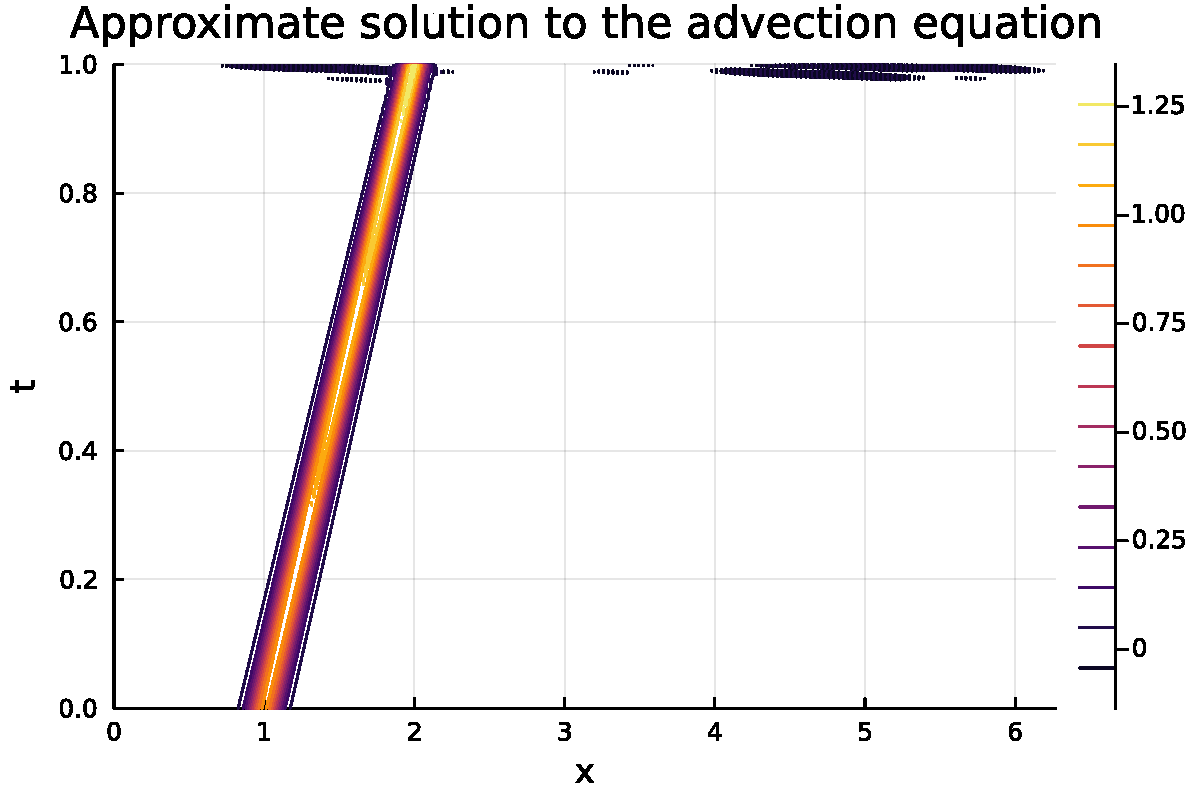
\includegraphics[width=\linewidth]{jl_fFQb2q/Fourier_14_1.pdf}

\begin{lstlisting}
(*@\HLJLnf{surface}@*)(*@\HLJLp{(}@*)(*@\HLJLn{x}@*)(*@\HLJLp{,}@*)(*@\HLJLn{t}@*)(*@\HLJLp{,}@*)(*@\HLJLn{u}@*)(*@\HLJLp{;}@*)(*@\HLJLn{seriescolor}@*)(*@\HLJLoB{=:}@*)(*@\HLJLn{redsblues}@*)(*@\HLJLp{,}@*) (*@\HLJLn{camera}@*)(*@\HLJLoB{=}@*)(*@\HLJLp{(}@*)(*@\HLJLni{10}@*)(*@\HLJLp{,}@*)(*@\HLJLni{50}@*)(*@\HLJLp{),}@*)
(*@\HLJLn{xlabel}@*)(*@\HLJLoB{=}@*)(*@\HLJLs{"{}x"{}}@*)(*@\HLJLp{,}@*)(*@\HLJLn{ylabel}@*)(*@\HLJLoB{=}@*)(*@\HLJLs{"{}t"{}}@*)(*@\HLJLp{,}@*)(*@\HLJLn{title}@*)(*@\HLJLoB{=}@*)(*@\HLJLs{"{}Approximate}@*) (*@\HLJLs{solution}@*) (*@\HLJLs{to}@*) (*@\HLJLs{the}@*) (*@\HLJLs{advection}@*) (*@\HLJLs{equation"{}}@*)(*@\HLJLp{)}@*)
\end{lstlisting}

\includegraphics[width=\linewidth]{jl_fFQb2q/Fourier_15_1.pdf}

Note the spurious oscillations in the numerical solution.  We shall analyse why this instability occurs later in this module.  Whe shall also see that if we approximate the time derivative with a central difference, then we can take larger time steps while retaining stability. That is, if we use

\[
u_t(x_j,t_i) \approx \frac{u(x_j,t_{i+1}) - u(x_j,t_{i-1})}{2\tau} \approx \frac{u^{i+1}_j - u^{i-1}_j}{2\tau}, \qquad j = 0, \ldots, n_x-1
\]
and again approximate the spatial derivative via FFTs, then we obtain another numerical method for the advection equation:

\[
\mathbf{u}^{i+1} = \mathbf{u}^{i-1} - 2\tau \mathcal{F}^{-1}\left\lbrace {\rm i}(-m\!:\!m)\cdot\mathcal{F}\lbrace \mathbf{u}^{i} \rbrace\right\rbrace, \qquad i = 0, \ldots, n_t-1, \qquad \mathbf{u}^0 = \mathbf{f}.
\]
This is known as a leap frog method.

We have $\mathbf{u}^0$, however we also need $\mathbf{u}^1$ to implement the leap frog method.  There are various one-step methods one could use to obtain $\mathbf{u}^1$ from $\mathbf{u}^0$ (e.g., Runge-Kutta methods, which we might get to later) but here we use 10 steps of the forward difference method above with step size $\tau/10$:


\begin{lstlisting}
(*@\HLJLn{n\ensuremath{\_t}}@*) (*@\HLJLoB{=}@*) (*@\HLJLni{500}@*)
(*@\HLJLn{T}@*) (*@\HLJLoB{=}@*) (*@\HLJLnfB{2.5}@*)
(*@\HLJLn{\ensuremath{\tau}}@*) (*@\HLJLoB{=}@*) (*@\HLJLn{T}@*)(*@\HLJLoB{/}@*)(*@\HLJLn{n\ensuremath{\_t}}@*)
(*@\HLJLn{u}@*) (*@\HLJLoB{=}@*) (*@\HLJLnf{zeros}@*)(*@\HLJLp{(}@*)(*@\HLJLn{n\ensuremath{\_t}}@*) (*@\HLJLoB{+}@*) (*@\HLJLni{1}@*)(*@\HLJLp{,}@*)(*@\HLJLn{n\ensuremath{\_x}}@*)(*@\HLJLp{)}@*)
(*@\HLJLn{u}@*)(*@\HLJLp{[}@*)(*@\HLJLni{1}@*)(*@\HLJLp{,}@*)(*@\HLJLoB{:}@*)(*@\HLJLp{]}@*) (*@\HLJLoB{=}@*) (*@\HLJLn{f}@*)(*@\HLJLoB{.}@*)(*@\HLJLp{(}@*)(*@\HLJLn{x}@*)(*@\HLJLp{)}@*) 

(*@\HLJLcs{{\#}}@*) (*@\HLJLcs{First}@*) (*@\HLJLcs{take}@*) (*@\HLJLcs{ten}@*) (*@\HLJLcs{steps}@*) (*@\HLJLcs{using}@*) (*@\HLJLcs{the}@*) (*@\HLJLcs{forward}@*) (*@\HLJLcs{difference}@*) (*@\HLJLcs{formula}@*)
(*@\HLJLn{ut}@*) (*@\HLJLoB{=}@*) (*@\HLJLnf{zeros}@*)(*@\HLJLp{(}@*)(*@\HLJLni{11}@*)(*@\HLJLp{,}@*)(*@\HLJLn{n\ensuremath{\_x}}@*)(*@\HLJLp{)}@*)
(*@\HLJLn{u}@*)(*@\HLJLp{[}@*)(*@\HLJLni{1}@*)(*@\HLJLp{,}@*)(*@\HLJLoB{:}@*)(*@\HLJLp{]}@*) (*@\HLJLoB{=}@*) (*@\HLJLn{ut}@*)(*@\HLJLp{[}@*)(*@\HLJLni{1}@*)(*@\HLJLp{,}@*)(*@\HLJLoB{:}@*)(*@\HLJLp{]}@*) (*@\HLJLoB{=}@*)  (*@\HLJLn{f}@*)(*@\HLJLoB{.}@*)(*@\HLJLp{(}@*)(*@\HLJLn{x}@*)(*@\HLJLp{)}@*) (*@\HLJLcs{{\#}}@*) (*@\HLJLcs{initial}@*) (*@\HLJLcs{data}@*)
(*@\HLJLk{for}@*) (*@\HLJLn{n}@*) (*@\HLJLoB{=}@*) (*@\HLJLni{1}@*)(*@\HLJLoB{:}@*)(*@\HLJLni{10}@*)
    (*@\HLJLn{ut}@*)(*@\HLJLp{[}@*)(*@\HLJLn{n}@*)(*@\HLJLoB{+}@*)(*@\HLJLni{1}@*)(*@\HLJLp{,}@*)(*@\HLJLoB{:}@*)(*@\HLJLp{]}@*) (*@\HLJLoB{=}@*) (*@\HLJLn{real}@*)(*@\HLJLoB{.}@*)(*@\HLJLp{(}@*)(*@\HLJLn{ut}@*)(*@\HLJLp{[}@*)(*@\HLJLn{n}@*)(*@\HLJLp{,}@*)(*@\HLJLoB{:}@*)(*@\HLJLp{]}@*) (*@\HLJLoB{-}@*) (*@\HLJLn{\ensuremath{\tau}}@*)(*@\HLJLoB{/}@*)(*@\HLJLni{10}@*)(*@\HLJLoB{*}@*)(*@\HLJLnf{ifft}@*)(*@\HLJLp{(}@*)(*@\HLJLnf{ifftshift}@*)(*@\HLJLp{(}@*)(*@\HLJLn{im}@*)(*@\HLJLoB{*}@*)(*@\HLJLp{(}@*)(*@\HLJLoB{-}@*)(*@\HLJLn{m}@*)(*@\HLJLoB{:}@*)(*@\HLJLn{m}@*)(*@\HLJLp{))}@*)(*@\HLJLoB{.*}@*)(*@\HLJLnf{fft}@*)(*@\HLJLp{(}@*)(*@\HLJLn{ut}@*)(*@\HLJLp{[}@*)(*@\HLJLn{n}@*)(*@\HLJLp{,}@*)(*@\HLJLoB{:}@*)(*@\HLJLp{])))}@*)
(*@\HLJLk{end}@*)

(*@\HLJLcs{{\#}}@*) (*@\HLJLcs{Now}@*) (*@\HLJLcs{use}@*) (*@\HLJLcs{the}@*) (*@\HLJLcs{leap}@*) (*@\HLJLcs{frog}@*) (*@\HLJLcs{method}@*)
(*@\HLJLn{u}@*)(*@\HLJLp{[}@*)(*@\HLJLni{2}@*)(*@\HLJLp{,}@*)(*@\HLJLoB{:}@*)(*@\HLJLp{]}@*) (*@\HLJLoB{=}@*) (*@\HLJLn{ut}@*)(*@\HLJLp{[}@*)(*@\HLJLni{11}@*)(*@\HLJLp{,}@*)(*@\HLJLoB{:}@*)(*@\HLJLp{]}@*)
(*@\HLJLk{for}@*) (*@\HLJLn{n}@*) (*@\HLJLoB{=}@*) (*@\HLJLni{2}@*)(*@\HLJLoB{:}@*)(*@\HLJLn{n\ensuremath{\_t}}@*)(*@\HLJLoB{-}@*)(*@\HLJLni{1}@*)
    (*@\HLJLn{u}@*)(*@\HLJLp{[}@*)(*@\HLJLn{n}@*)(*@\HLJLoB{+}@*)(*@\HLJLni{1}@*)(*@\HLJLp{,}@*)(*@\HLJLoB{:}@*)(*@\HLJLp{]}@*) (*@\HLJLoB{=}@*) (*@\HLJLn{real}@*)(*@\HLJLoB{.}@*)(*@\HLJLp{(}@*)(*@\HLJLn{u}@*)(*@\HLJLp{[}@*)(*@\HLJLn{n}@*)(*@\HLJLoB{-}@*)(*@\HLJLni{1}@*)(*@\HLJLp{,}@*)(*@\HLJLoB{:}@*)(*@\HLJLp{]}@*) (*@\HLJLoB{-}@*) (*@\HLJLni{2}@*)(*@\HLJLn{\ensuremath{\tau}}@*)(*@\HLJLoB{*}@*)(*@\HLJLnf{ifft}@*)(*@\HLJLp{(}@*)(*@\HLJLnf{ifftshift}@*)(*@\HLJLp{(}@*)(*@\HLJLn{im}@*)(*@\HLJLoB{*}@*)(*@\HLJLp{(}@*)(*@\HLJLoB{-}@*)(*@\HLJLn{m}@*)(*@\HLJLoB{:}@*)(*@\HLJLn{m}@*)(*@\HLJLp{))}@*)(*@\HLJLoB{.*}@*)(*@\HLJLnf{fft}@*)(*@\HLJLp{(}@*)(*@\HLJLn{u}@*)(*@\HLJLp{[}@*)(*@\HLJLn{n}@*)(*@\HLJLp{,}@*)(*@\HLJLoB{:}@*)(*@\HLJLp{])))}@*)
(*@\HLJLk{end}@*)
\end{lstlisting}


\begin{lstlisting}
(*@\HLJLn{t}@*) (*@\HLJLoB{=}@*) (*@\HLJLnf{range}@*)(*@\HLJLp{(}@*)(*@\HLJLni{0}@*)(*@\HLJLp{,}@*)(*@\HLJLn{T}@*)(*@\HLJLp{;}@*)(*@\HLJLn{length}@*)(*@\HLJLoB{=}@*)(*@\HLJLn{n\ensuremath{\_t}}@*)(*@\HLJLoB{+}@*)(*@\HLJLni{1}@*)(*@\HLJLp{)}@*)
(*@\HLJLnf{contour}@*)(*@\HLJLp{(}@*)(*@\HLJLn{x}@*)(*@\HLJLp{,}@*)(*@\HLJLn{t}@*)(*@\HLJLp{,}@*)(*@\HLJLn{u}@*)(*@\HLJLp{;}@*)(*@\HLJLn{xlabel}@*)(*@\HLJLoB{=}@*)(*@\HLJLs{"{}x"{}}@*)(*@\HLJLp{,}@*)(*@\HLJLn{ylabel}@*)(*@\HLJLoB{=}@*)(*@\HLJLs{"{}t"{}}@*)(*@\HLJLp{,}@*)(*@\HLJLn{title}@*)(*@\HLJLoB{=}@*)(*@\HLJLs{"{}Leapfrog}@*) (*@\HLJLs{solution}@*) (*@\HLJLs{to}@*) (*@\HLJLs{the}@*) (*@\HLJLs{advection}@*) (*@\HLJLs{equation"{}}@*)(*@\HLJLp{)}@*)
\end{lstlisting}

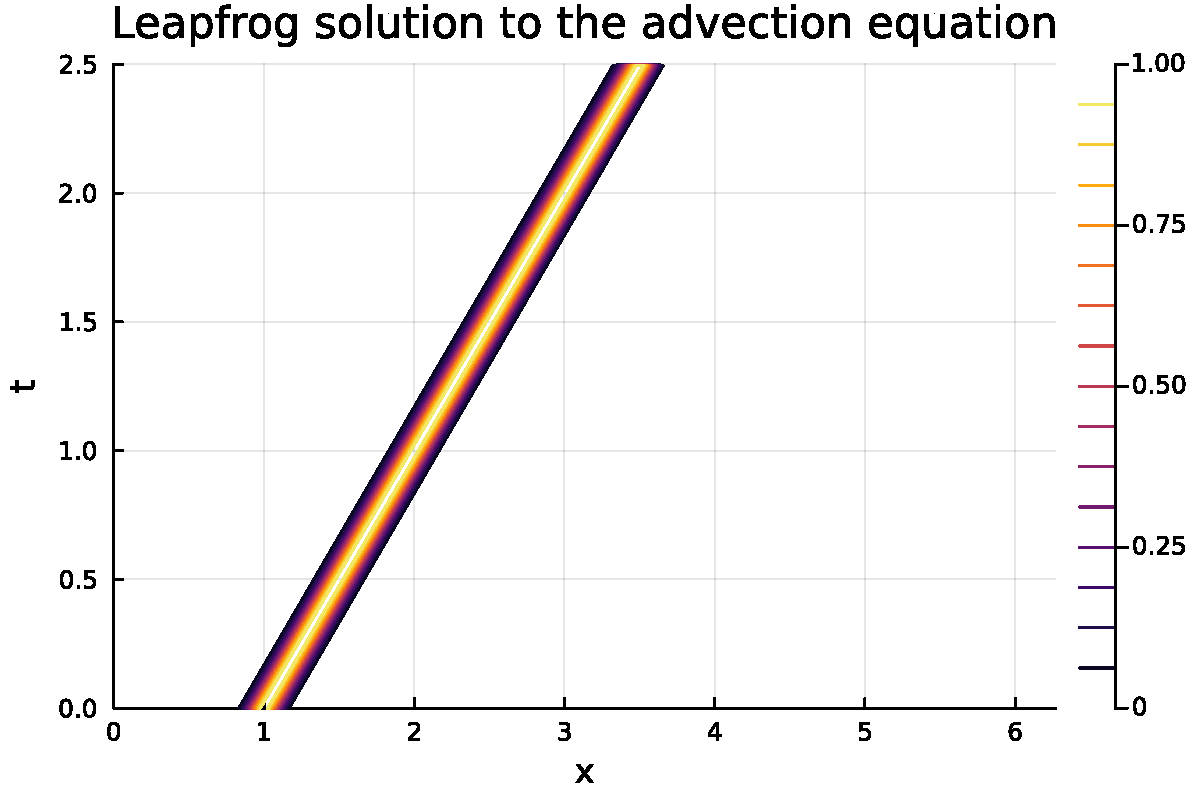
\includegraphics[width=\linewidth]{jl_fFQb2q/Fourier_17_1.pdf}

\begin{lstlisting}
(*@\HLJLnf{surface}@*)(*@\HLJLp{(}@*)(*@\HLJLn{x}@*)(*@\HLJLp{,}@*)(*@\HLJLn{t}@*)(*@\HLJLp{,}@*)(*@\HLJLn{u}@*)(*@\HLJLp{;}@*)(*@\HLJLn{seriescolor}@*)(*@\HLJLoB{=:}@*)(*@\HLJLn{redsblues}@*)(*@\HLJLp{,}@*) (*@\HLJLn{camera}@*)(*@\HLJLoB{=}@*)(*@\HLJLp{(}@*)(*@\HLJLni{10}@*)(*@\HLJLp{,}@*)(*@\HLJLni{50}@*)(*@\HLJLp{),}@*)
(*@\HLJLn{xlabel}@*)(*@\HLJLoB{=}@*)(*@\HLJLs{"{}x"{}}@*)(*@\HLJLp{,}@*)(*@\HLJLn{ylabel}@*)(*@\HLJLoB{=}@*)(*@\HLJLs{"{}t"{}}@*)(*@\HLJLp{,}@*)(*@\HLJLn{title}@*)(*@\HLJLoB{=}@*)(*@\HLJLs{"{}Leapfrog}@*) (*@\HLJLs{solution}@*) (*@\HLJLs{to}@*) (*@\HLJLs{the}@*) (*@\HLJLs{advection}@*) (*@\HLJLs{equation"{}}@*)(*@\HLJLp{)}@*)
\end{lstlisting}

\includegraphics[width=\linewidth]{jl_fFQb2q/Fourier_18_1.pdf}

Let's consider now the advection equation with a variable coefficient:

\[
u_t + c(x)u_x = 0
\]
with 

\[
c(x) = \frac{1}{5} + \sin^2(x-1)
\]
and the same initial data as before, $u(x,0) = f(x) = {\rm e}^{-100(x-1)^2}$.  We can easily verify that the exact solution to this Cauchy problem (which can be derived using the method of characteristics) is 

\[
u(x,t) = f\left(t - C(x)  \right),
\]
where $C(x)$ is an antiderivative of $1/c(x)$, i.e., $C'(x) = 1/c(x)$.    For example,

\[
C(x) = -\frac{5}{\sqrt{6}}\arctan \left(\sqrt{6}\tan(1-x)  \right).
\]
If we again use central differences to approximate the time derivative and FFTs to approximate the spatial derivative, then the leapfrog method is

\[
\mathbf{u}^{i+1} = \mathbf{u}^{i-1} - 2\tau c(\mathbf{x})\cdot \mathcal{F}^{-1}\left\lbrace {\rm i}(-m\!:\!m)\cdot\mathcal{F}\lbrace \mathbf{u}^{i} \rbrace\right\rbrace, \qquad i = 0, \ldots, n_t-1, \qquad \mathbf{u}^0 = \mathbf{f}.
\]
As before, we'll use 10 steps of the forward difference method with a step size of $\tau/10$ to compute $\mathbf{u}^{1}$ to initialise the leapfrog method:


\begin{lstlisting}
(*@\HLJLn{c}@*) (*@\HLJLoB{=}@*) (*@\HLJLn{x}@*) (*@\HLJLoB{->}@*) (*@\HLJLnfB{0.2}@*) (*@\HLJLoB{+}@*) (*@\HLJLnf{sin}@*)(*@\HLJLp{(}@*)(*@\HLJLn{x}@*) (*@\HLJLoB{-}@*) (*@\HLJLni{1}@*)(*@\HLJLp{)}@*)(*@\HLJLoB{{\textasciicircum}}@*)(*@\HLJLni{2}@*)
(*@\HLJLn{n\ensuremath{\_t}}@*) (*@\HLJLoB{=}@*) (*@\HLJLni{2000}@*)
(*@\HLJLn{T}@*) (*@\HLJLoB{=}@*) (*@\HLJLni{8}@*)
(*@\HLJLn{\ensuremath{\tau}}@*) (*@\HLJLoB{=}@*) (*@\HLJLn{T}@*)(*@\HLJLoB{/}@*)(*@\HLJLn{n\ensuremath{\_t}}@*)
(*@\HLJLn{u}@*) (*@\HLJLoB{=}@*) (*@\HLJLnf{zeros}@*)(*@\HLJLp{(}@*)(*@\HLJLn{n\ensuremath{\_t}}@*) (*@\HLJLoB{+}@*) (*@\HLJLni{1}@*)(*@\HLJLp{,}@*)(*@\HLJLn{n\ensuremath{\_x}}@*)(*@\HLJLp{)}@*)
(*@\HLJLn{u}@*)(*@\HLJLp{[}@*)(*@\HLJLni{1}@*)(*@\HLJLp{,}@*)(*@\HLJLoB{:}@*)(*@\HLJLp{]}@*) (*@\HLJLoB{=}@*) (*@\HLJLn{f}@*)(*@\HLJLoB{.}@*)(*@\HLJLp{(}@*)(*@\HLJLn{x}@*)(*@\HLJLp{)}@*) 

(*@\HLJLcs{{\#}}@*) (*@\HLJLcs{First}@*) (*@\HLJLcs{take}@*) (*@\HLJLcs{ten}@*) (*@\HLJLcs{steps}@*) (*@\HLJLcs{using}@*) (*@\HLJLcs{the}@*) (*@\HLJLcs{forward}@*) (*@\HLJLcs{difference}@*) (*@\HLJLcs{formula}@*)
(*@\HLJLn{ut}@*) (*@\HLJLoB{=}@*) (*@\HLJLnf{zeros}@*)(*@\HLJLp{(}@*)(*@\HLJLni{11}@*)(*@\HLJLp{,}@*)(*@\HLJLn{n\ensuremath{\_x}}@*)(*@\HLJLp{)}@*)
(*@\HLJLn{u}@*)(*@\HLJLp{[}@*)(*@\HLJLni{1}@*)(*@\HLJLp{,}@*)(*@\HLJLoB{:}@*)(*@\HLJLp{]}@*) (*@\HLJLoB{=}@*) (*@\HLJLn{ut}@*)(*@\HLJLp{[}@*)(*@\HLJLni{1}@*)(*@\HLJLp{,}@*)(*@\HLJLoB{:}@*)(*@\HLJLp{]}@*) (*@\HLJLoB{=}@*)  (*@\HLJLn{f}@*)(*@\HLJLoB{.}@*)(*@\HLJLp{(}@*)(*@\HLJLn{x}@*)(*@\HLJLp{)}@*) (*@\HLJLcs{{\#}}@*) (*@\HLJLcs{initial}@*) (*@\HLJLcs{data}@*)
(*@\HLJLk{for}@*) (*@\HLJLn{n}@*) (*@\HLJLoB{=}@*) (*@\HLJLni{1}@*)(*@\HLJLoB{:}@*)(*@\HLJLni{10}@*)
    (*@\HLJLn{ut}@*)(*@\HLJLp{[}@*)(*@\HLJLn{n}@*)(*@\HLJLoB{+}@*)(*@\HLJLni{1}@*)(*@\HLJLp{,}@*)(*@\HLJLoB{:}@*)(*@\HLJLp{]}@*) (*@\HLJLoB{=}@*) (*@\HLJLn{real}@*)(*@\HLJLoB{.}@*)(*@\HLJLp{(}@*)(*@\HLJLn{ut}@*)(*@\HLJLp{[}@*)(*@\HLJLn{n}@*)(*@\HLJLp{,}@*)(*@\HLJLoB{:}@*)(*@\HLJLp{]}@*) (*@\HLJLoB{-}@*) (*@\HLJLn{\ensuremath{\tau}}@*)(*@\HLJLoB{/}@*)(*@\HLJLni{10}@*)(*@\HLJLoB{*}@*)(*@\HLJLn{c}@*)(*@\HLJLoB{.}@*)(*@\HLJLp{(}@*)(*@\HLJLn{x}@*)(*@\HLJLp{)}@*)(*@\HLJLoB{.*}@*)(*@\HLJLnf{ifft}@*)(*@\HLJLp{(}@*)(*@\HLJLnf{ifftshift}@*)(*@\HLJLp{(}@*)(*@\HLJLn{im}@*)(*@\HLJLoB{*}@*)(*@\HLJLp{(}@*)(*@\HLJLoB{-}@*)(*@\HLJLn{m}@*)(*@\HLJLoB{:}@*)(*@\HLJLn{m}@*)(*@\HLJLp{))}@*)(*@\HLJLoB{.*}@*)(*@\HLJLnf{fft}@*)(*@\HLJLp{(}@*)(*@\HLJLn{ut}@*)(*@\HLJLp{[}@*)(*@\HLJLn{n}@*)(*@\HLJLp{,}@*)(*@\HLJLoB{:}@*)(*@\HLJLp{])))}@*)
(*@\HLJLk{end}@*)

(*@\HLJLcs{{\#}}@*) (*@\HLJLcs{Now}@*) (*@\HLJLcs{use}@*) (*@\HLJLcs{the}@*) (*@\HLJLcs{leap}@*) (*@\HLJLcs{frog}@*) (*@\HLJLcs{method}@*)
(*@\HLJLn{u}@*)(*@\HLJLp{[}@*)(*@\HLJLni{2}@*)(*@\HLJLp{,}@*)(*@\HLJLoB{:}@*)(*@\HLJLp{]}@*) (*@\HLJLoB{=}@*) (*@\HLJLn{ut}@*)(*@\HLJLp{[}@*)(*@\HLJLni{11}@*)(*@\HLJLp{,}@*)(*@\HLJLoB{:}@*)(*@\HLJLp{]}@*)
(*@\HLJLk{for}@*) (*@\HLJLn{n}@*) (*@\HLJLoB{=}@*) (*@\HLJLni{2}@*)(*@\HLJLoB{:}@*)(*@\HLJLn{n\ensuremath{\_t}}@*)(*@\HLJLoB{-}@*)(*@\HLJLni{1}@*)
    (*@\HLJLn{u}@*)(*@\HLJLp{[}@*)(*@\HLJLn{n}@*)(*@\HLJLoB{+}@*)(*@\HLJLni{1}@*)(*@\HLJLp{,}@*)(*@\HLJLoB{:}@*)(*@\HLJLp{]}@*) (*@\HLJLoB{=}@*) (*@\HLJLn{real}@*)(*@\HLJLoB{.}@*)(*@\HLJLp{(}@*)(*@\HLJLn{u}@*)(*@\HLJLp{[}@*)(*@\HLJLn{n}@*)(*@\HLJLoB{-}@*)(*@\HLJLni{1}@*)(*@\HLJLp{,}@*)(*@\HLJLoB{:}@*)(*@\HLJLp{]}@*) (*@\HLJLoB{-}@*) (*@\HLJLni{2}@*)(*@\HLJLn{\ensuremath{\tau}}@*)(*@\HLJLoB{*}@*)(*@\HLJLn{c}@*)(*@\HLJLoB{.}@*)(*@\HLJLp{(}@*)(*@\HLJLn{x}@*)(*@\HLJLp{)}@*)(*@\HLJLoB{.*}@*)(*@\HLJLnf{ifft}@*)(*@\HLJLp{(}@*)(*@\HLJLnf{ifftshift}@*)(*@\HLJLp{(}@*)(*@\HLJLn{im}@*)(*@\HLJLoB{*}@*)(*@\HLJLp{(}@*)(*@\HLJLoB{-}@*)(*@\HLJLn{m}@*)(*@\HLJLoB{:}@*)(*@\HLJLn{m}@*)(*@\HLJLp{))}@*)(*@\HLJLoB{.*}@*)(*@\HLJLnf{fft}@*)(*@\HLJLp{(}@*)(*@\HLJLn{u}@*)(*@\HLJLp{[}@*)(*@\HLJLn{n}@*)(*@\HLJLp{,}@*)(*@\HLJLoB{:}@*)(*@\HLJLp{])))}@*)
(*@\HLJLk{end}@*)
\end{lstlisting}


\begin{lstlisting}
(*@\HLJLn{t}@*) (*@\HLJLoB{=}@*) (*@\HLJLnf{range}@*)(*@\HLJLp{(}@*)(*@\HLJLni{0}@*)(*@\HLJLp{,}@*)(*@\HLJLn{T}@*)(*@\HLJLp{;}@*)(*@\HLJLn{length}@*)(*@\HLJLoB{=}@*)(*@\HLJLn{n\ensuremath{\_t}}@*)(*@\HLJLoB{+}@*)(*@\HLJLni{1}@*)(*@\HLJLp{)}@*)
(*@\HLJLnf{contour}@*)(*@\HLJLp{(}@*)(*@\HLJLn{x}@*)(*@\HLJLp{,}@*)(*@\HLJLn{t}@*)(*@\HLJLp{,}@*)(*@\HLJLn{u}@*)(*@\HLJLp{;}@*)(*@\HLJLn{xlabel}@*)(*@\HLJLoB{=}@*)(*@\HLJLs{"{}x"{}}@*)(*@\HLJLp{,}@*)(*@\HLJLn{ylabel}@*)(*@\HLJLoB{=}@*)(*@\HLJLs{"{}t"{}}@*)(*@\HLJLp{,}@*)(*@\HLJLn{title}@*)(*@\HLJLoB{=}@*)(*@\HLJLs{"{}Leapfrog}@*) (*@\HLJLs{sln}@*) (*@\HLJLs{to}@*) (*@\HLJLs{the}@*) (*@\HLJLs{variable}@*) (*@\HLJLs{coefficient}@*) (*@\HLJLs{advection}@*) (*@\HLJLs{eqn"{}}@*)(*@\HLJLp{)}@*)
\end{lstlisting}

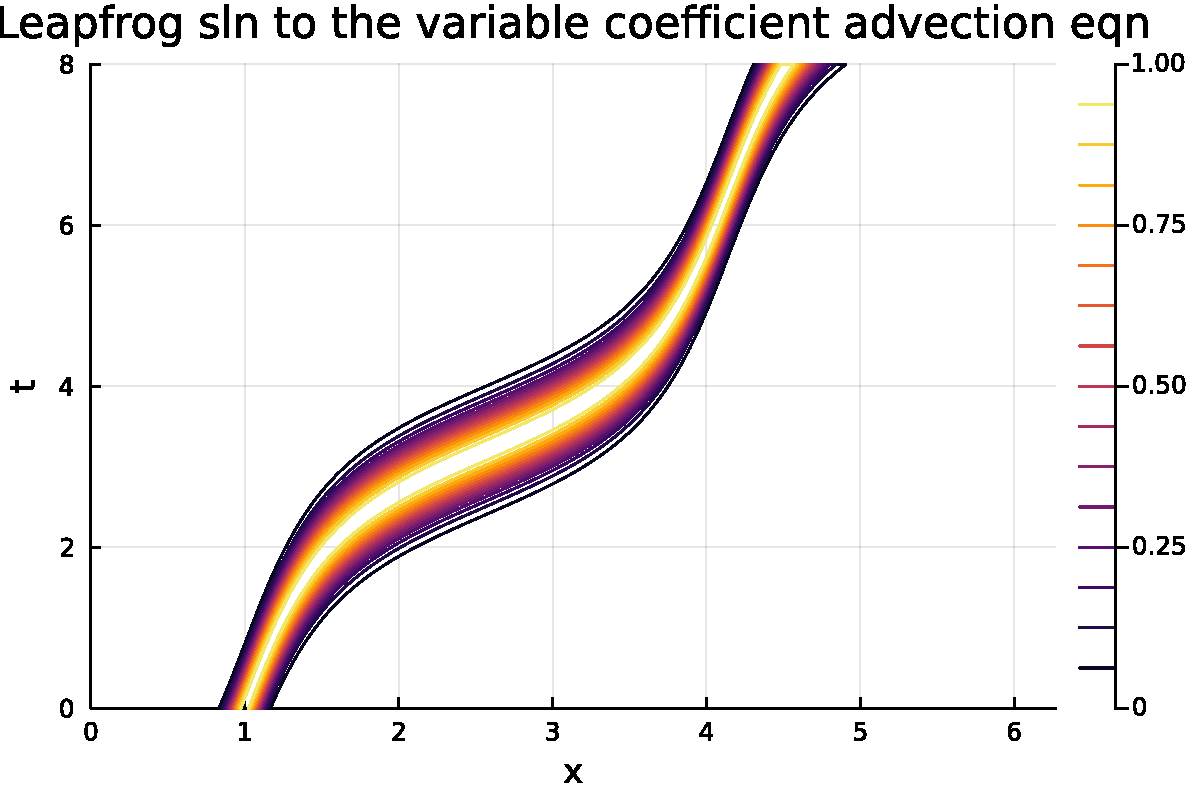
\includegraphics[width=\linewidth]{jl_fFQb2q/Fourier_20_1.pdf}

\begin{lstlisting}
(*@\HLJLnf{surface}@*)(*@\HLJLp{(}@*)(*@\HLJLn{x}@*)(*@\HLJLp{,}@*)(*@\HLJLn{t}@*)(*@\HLJLp{,}@*)(*@\HLJLn{u}@*)(*@\HLJLp{;}@*)(*@\HLJLn{seriescolor}@*)(*@\HLJLoB{=:}@*)(*@\HLJLn{redsblues}@*)(*@\HLJLp{,}@*) (*@\HLJLn{camera}@*)(*@\HLJLoB{=}@*)(*@\HLJLp{(}@*)(*@\HLJLni{10}@*)(*@\HLJLp{,}@*)(*@\HLJLni{50}@*)(*@\HLJLp{),}@*)
(*@\HLJLn{xlabel}@*)(*@\HLJLoB{=}@*)(*@\HLJLs{"{}x"{}}@*)(*@\HLJLp{,}@*)(*@\HLJLn{ylabel}@*)(*@\HLJLoB{=}@*)(*@\HLJLs{"{}t"{}}@*)(*@\HLJLp{,}@*)(*@\HLJLn{title}@*)(*@\HLJLoB{=}@*)(*@\HLJLs{"{}Leapfrog}@*) (*@\HLJLs{sln}@*) (*@\HLJLs{to}@*) (*@\HLJLs{the}@*) (*@\HLJLs{variable}@*) (*@\HLJLs{coefficient}@*) (*@\HLJLs{advection}@*) (*@\HLJLs{eqn"{}}@*)(*@\HLJLp{)}@*)
\end{lstlisting}

\includegraphics[width=\linewidth]{jl_fFQb2q/Fourier_21_1.pdf}

\subsection{Smoothness of $f$ and decay of Fourier coefficients}
What happens if we approximate a function that is not periodic with the periodic interpolant

\[
p(x) = \sum_{k=-m}^{m}\widetilde{c}_k{\rm e}^{{\rm i}kx}?
\]
\textbf{Example} Consider the function $f(x) = {\rm e}^{x-2\pi}$. This function is not  $2\pi$-periodic because $f(x + 2\pi) \neq f(x)$. However, for any function $f$, we can define its \emph{periodic extension}

\[
f(x + 2\pi p) = f(x), \qquad x \in [0, 2\pi), \qquad p \in \mathbb{Z},
\]
which is a $2\pi$-periodic function.  Here is a plot of the periodic extension of $f$ on $[-2\pi, 4\pi]$, however it extends infinitely far to the left and right.


\begin{lstlisting}
(*@\HLJLn{f\ensuremath{\_1}}@*) (*@\HLJLoB{=}@*) (*@\HLJLn{x}@*) (*@\HLJLoB{->}@*) (*@\HLJLnf{exp}@*)(*@\HLJLp{(}@*)(*@\HLJLn{x}@*)(*@\HLJLoB{-}@*)(*@\HLJLni{2}@*)(*@\HLJLn{\ensuremath{\pi}}@*)(*@\HLJLp{)}@*)
(*@\HLJLn{xx}@*) (*@\HLJLoB{=}@*) (*@\HLJLnf{range}@*)(*@\HLJLp{(}@*)(*@\HLJLni{0}@*)(*@\HLJLp{,}@*)(*@\HLJLni{2}@*)(*@\HLJLn{\ensuremath{\pi}}@*)(*@\HLJLp{;}@*)(*@\HLJLn{length}@*)(*@\HLJLoB{=}@*)(*@\HLJLni{501}@*)(*@\HLJLp{)[}@*)(*@\HLJLni{1}@*)(*@\HLJLoB{:}@*)(*@\HLJLk{end}@*)(*@\HLJLoB{-}@*)(*@\HLJLni{1}@*)(*@\HLJLp{]}@*) (*@\HLJLcs{{\#}}@*) (*@\HLJLcs{plotting}@*) (*@\HLJLcs{grid}@*)
(*@\HLJLnf{plot}@*)(*@\HLJLp{(}@*)(*@\HLJLn{xx}@*)(*@\HLJLp{,}@*)(*@\HLJLn{f\ensuremath{\_1}}@*)(*@\HLJLoB{.}@*)(*@\HLJLp{(}@*)(*@\HLJLn{xx}@*)(*@\HLJLp{);}@*)(*@\HLJLn{lw}@*)(*@\HLJLoB{=}@*)(*@\HLJLni{3}@*)(*@\HLJLp{,}@*)(*@\HLJLn{lc}@*)(*@\HLJLoB{=:}@*)(*@\HLJLn{blue}@*)(*@\HLJLp{,}@*)(*@\HLJLn{legend}@*)(*@\HLJLoB{=}@*)(*@\HLJLkc{false}@*)(*@\HLJLp{)}@*)
(*@\HLJLnf{plot!}@*)(*@\HLJLp{(}@*)(*@\HLJLn{xx}@*) (*@\HLJLoB{.+}@*) (*@\HLJLni{2}@*)(*@\HLJLn{\ensuremath{\pi}}@*)(*@\HLJLp{,}@*)(*@\HLJLn{f\ensuremath{\_1}}@*)(*@\HLJLoB{.}@*)(*@\HLJLp{(}@*)(*@\HLJLn{xx}@*)(*@\HLJLp{);}@*)(*@\HLJLn{lw}@*)(*@\HLJLoB{=}@*)(*@\HLJLni{3}@*)(*@\HLJLp{,}@*)(*@\HLJLn{lc}@*)(*@\HLJLoB{=:}@*)(*@\HLJLn{blue}@*)(*@\HLJLp{,}@*)(*@\HLJLn{legend}@*)(*@\HLJLoB{=}@*)(*@\HLJLkc{false}@*)(*@\HLJLp{)}@*)
(*@\HLJLnf{plot!}@*)(*@\HLJLp{(}@*)(*@\HLJLn{xx}@*) (*@\HLJLoB{.-}@*) (*@\HLJLni{2}@*)(*@\HLJLn{\ensuremath{\pi}}@*)(*@\HLJLp{,}@*)(*@\HLJLn{f\ensuremath{\_1}}@*)(*@\HLJLoB{.}@*)(*@\HLJLp{(}@*)(*@\HLJLn{xx}@*)(*@\HLJLp{);}@*)(*@\HLJLn{lw}@*)(*@\HLJLoB{=}@*)(*@\HLJLni{3}@*)(*@\HLJLp{,}@*)(*@\HLJLn{lc}@*)(*@\HLJLoB{=:}@*)(*@\HLJLn{blue}@*)(*@\HLJLp{,}@*)(*@\HLJLn{legend}@*)(*@\HLJLoB{=}@*)(*@\HLJLkc{false}@*)(*@\HLJLp{)}@*)
\end{lstlisting}

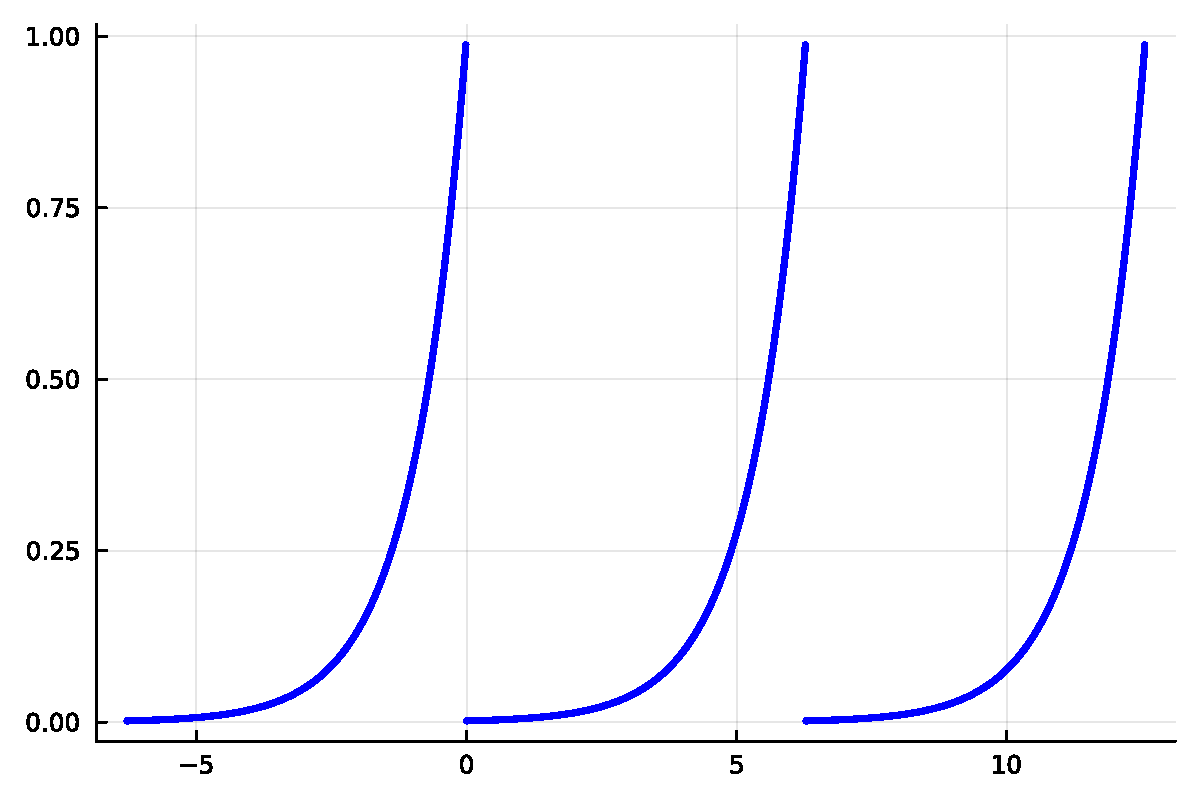
\includegraphics[width=\linewidth]{jl_fFQb2q/Fourier_22_1.pdf}

Notice that the periodic extension has jump discontinuities at $x = 2\pi p$, $p \in \mathbb{Z}$.

Here is the trigonometric interpolant of the periodic extension of $f$:


\begin{lstlisting}
(*@\HLJLnf{plot}@*)(*@\HLJLp{(}@*)(*@\HLJLn{xx}@*)(*@\HLJLp{,}@*)(*@\HLJLn{f\ensuremath{\_1}}@*)(*@\HLJLoB{.}@*)(*@\HLJLp{(}@*)(*@\HLJLn{xx}@*)(*@\HLJLp{);}@*)(*@\HLJLn{lw}@*)(*@\HLJLoB{=}@*)(*@\HLJLni{3}@*)(*@\HLJLp{,}@*)(*@\HLJLn{lc}@*)(*@\HLJLoB{=:}@*)(*@\HLJLn{blue}@*)(*@\HLJLp{,}@*)(*@\HLJLn{legend}@*)(*@\HLJLoB{=}@*)(*@\HLJLkc{false}@*)(*@\HLJLp{)}@*)
(*@\HLJLnf{plot!}@*)(*@\HLJLp{(}@*)(*@\HLJLn{xx}@*) (*@\HLJLoB{.+}@*) (*@\HLJLni{2}@*)(*@\HLJLn{\ensuremath{\pi}}@*)(*@\HLJLp{,}@*)(*@\HLJLn{f\ensuremath{\_1}}@*)(*@\HLJLoB{.}@*)(*@\HLJLp{(}@*)(*@\HLJLn{xx}@*)(*@\HLJLp{);}@*)(*@\HLJLn{lw}@*)(*@\HLJLoB{=}@*)(*@\HLJLni{3}@*)(*@\HLJLp{,}@*)(*@\HLJLn{lc}@*)(*@\HLJLoB{=:}@*)(*@\HLJLn{blue}@*)(*@\HLJLp{,}@*)(*@\HLJLn{legend}@*)(*@\HLJLoB{=}@*)(*@\HLJLkc{false}@*)(*@\HLJLp{)}@*)
(*@\HLJLnf{plot!}@*)(*@\HLJLp{(}@*)(*@\HLJLn{xx}@*) (*@\HLJLoB{.-}@*) (*@\HLJLni{2}@*)(*@\HLJLn{\ensuremath{\pi}}@*)(*@\HLJLp{,}@*)(*@\HLJLn{f\ensuremath{\_1}}@*)(*@\HLJLoB{.}@*)(*@\HLJLp{(}@*)(*@\HLJLn{xx}@*)(*@\HLJLp{);}@*)(*@\HLJLn{lw}@*)(*@\HLJLoB{=}@*)(*@\HLJLni{3}@*)(*@\HLJLp{,}@*)(*@\HLJLn{lc}@*)(*@\HLJLoB{=:}@*)(*@\HLJLn{blue}@*)(*@\HLJLp{,}@*)(*@\HLJLn{legend}@*)(*@\HLJLoB{=}@*)(*@\HLJLkc{false}@*)(*@\HLJLp{)}@*)

(*@\HLJLcs{{\#}}@*) (*@\HLJLcs{Trigonometric}@*) (*@\HLJLcs{interpolant}@*)
(*@\HLJLn{n}@*) (*@\HLJLoB{=}@*) (*@\HLJLni{51}@*)
(*@\HLJLn{x}@*) (*@\HLJLoB{=}@*) (*@\HLJLnf{range}@*)(*@\HLJLp{(}@*)(*@\HLJLni{0}@*)(*@\HLJLp{,}@*)(*@\HLJLni{2}@*)(*@\HLJLn{\ensuremath{\pi}}@*)(*@\HLJLp{;}@*)(*@\HLJLn{length}@*)(*@\HLJLoB{=}@*)(*@\HLJLn{n}@*)(*@\HLJLoB{+}@*)(*@\HLJLni{1}@*)(*@\HLJLp{)[}@*)(*@\HLJLni{1}@*)(*@\HLJLoB{:}@*)(*@\HLJLk{end}@*)(*@\HLJLoB{-}@*)(*@\HLJLni{1}@*)(*@\HLJLp{]}@*)
(*@\HLJLn{c}@*) (*@\HLJLoB{=}@*) (*@\HLJLnf{fft}@*)(*@\HLJLp{(}@*)(*@\HLJLn{f\ensuremath{\_1}}@*)(*@\HLJLoB{.}@*)(*@\HLJLp{(}@*)(*@\HLJLn{x}@*)(*@\HLJLp{))}@*)(*@\HLJLoB{/}@*)(*@\HLJLn{n}@*)
(*@\HLJLn{p}@*) (*@\HLJLoB{=}@*) (*@\HLJLn{x}@*) (*@\HLJLoB{->}@*) (*@\HLJLnf{triginterp}@*)(*@\HLJLp{(}@*)(*@\HLJLn{c}@*)(*@\HLJLp{,}@*) (*@\HLJLn{x}@*)(*@\HLJLp{)}@*)
(*@\HLJLnf{plot!}@*)(*@\HLJLp{(}@*)(*@\HLJLn{xx}@*)(*@\HLJLp{,}@*)(*@\HLJLn{real}@*)(*@\HLJLoB{.}@*)(*@\HLJLp{(}@*)(*@\HLJLn{p}@*)(*@\HLJLoB{.}@*)(*@\HLJLp{(}@*)(*@\HLJLn{xx}@*)(*@\HLJLp{)),}@*)(*@\HLJLn{lw}@*)(*@\HLJLoB{=}@*)(*@\HLJLnfB{1.5}@*)(*@\HLJLp{,}@*)(*@\HLJLn{lc}@*)(*@\HLJLoB{=:}@*)(*@\HLJLn{red}@*)(*@\HLJLp{)}@*)
\end{lstlisting}

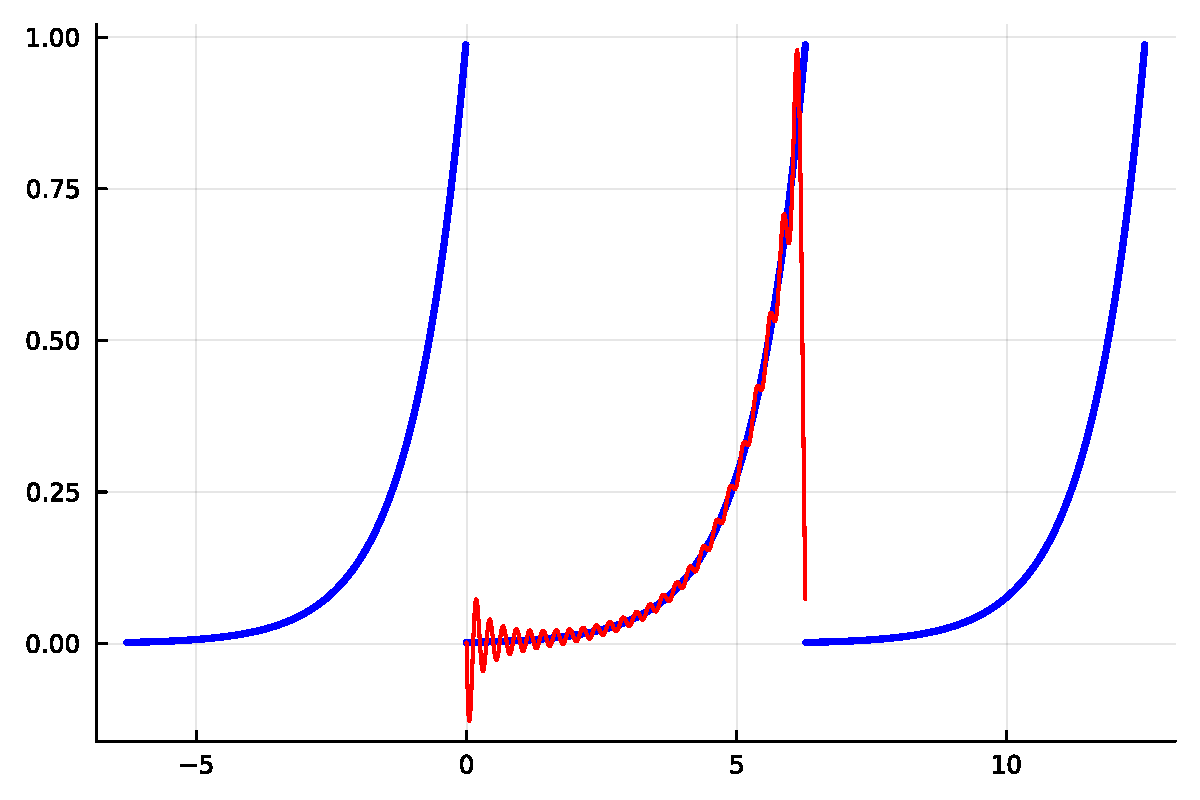
\includegraphics[width=\linewidth]{jl_fFQb2q/Fourier_23_1.pdf}

The periodic interpolant is clearly not a good approximation to the function.  The oscillations at the endpoints is known as the \emph{Gibbs phenomenon}.  As $n \to \infty$, the amplitude of the oscillations decrease as $\mathcal{O}(n^{-1})$ (very slowly) and the interpolant at $x=0$ and $x =2\pi$ converges to the average of the function values at  $x=0$ and $x =2\pi$:

\[
\lim_{x\to 0, 2\pi}p(x) = \frac{1}{2}\left(\lim_{x \to 0^{+}}f(x) + \lim_{x \to 2\pi^{-}}f(x)\right), \qquad n \to \infty.
\]
The reason why $p$ is not a good approximation to $f$ is because it is not very smooth (it has jump discontinuities, so it's $0$-th derivative is discontinuous). Our aim in this section is to relate the smoothness of $f$ to the accuracy of its approximation by the interpolant $p(x)$.  Then we'll be able to relate the smoothness of derivatives of $f$ to the accuracy of their approximation by derivatives of the interpolant, which is relevant to the analysis of the accuracy of spectral methods for PDEs.

We now show that the accuracy of the interpolant $p(x)$ and its derivatives depends on the magnitudes of the Fourier coefficients of the function $f$. It follows that


\begin{eqnarray*}
f^{(\nu)}(x) - p^{(\nu)}(x) & = & \sum_{k=-\infty}^{\infty}({\rm i}k)^{\nu}c_k{\rm e}^{{\rm i}kx} - \sum_{k=-m}^{m}({\rm i}k)^{\nu}\,\widetilde{c}_k{\rm e}^{{\rm i}kx} \\
 &=& \sum_{k=-m}^{m}({\rm i}k)^{\nu}\left(c_k - \widetilde{c}_k\right){\rm e}^{{\rm i}kx} + \sum_{\vert k \vert > m} ({\rm i}k)^{\nu}c_k{\rm e}^{{\rm i}kx}
\end{eqnarray*}
Recall that the approximate Fourier coefficients $\widetilde{c}_k$ that we obtain from the trapezoidal rule and the exact Fourier coefficients are related as follows:

\[
\widetilde{c}_k = \cdots + c_{k-2n} + c_{k-n} +  c_k +  c_{k+n} + c_{k+2n} + \cdots
\]
Therefore,


\begin{eqnarray}
\left\vert f^{(\nu)}(x) - p^{(\nu)}(x) \right\vert & \leq &  \sum_{k=-m}^{m} \vert k\vert^{\nu}\left\vert c_k - \widetilde{c}_k\right\vert + \sum_{\vert k \vert > m} \vert k \vert^{\nu} \vert c_k \vert \leq  2\sum_{\vert k \vert > m} \vert k \vert^{\nu} \vert c_k \vert 
\end{eqnarray}
The infinity norm of a function $g(x)$ on $[0, 2\pi]$ is defined as $\| g \|_{\infty} = \mathrm{sup}_{x\in[0,2\pi]} \vert g(x) \vert$, hence we have

\[
\| f^{(\nu)} - p^{(\nu)}  \|_{\infty} \leq  2\sum_{\vert k \vert > m} \vert k \vert^{\nu} \vert c_k \vert 
\]
Now we show that the magnitudes of the Fourier coefficients depend on the smoothness of $f$. First, we define the one-norm of a function $g(x)$ on $[0, 2\pi)$ by

\[
\| g \|_1 = \int_{0}^{2\pi}  \vert g(x) \vert \, {\rm d}x. 
\]
Also, we define $g(a^{-})$ as follows:

\[
g(a^{-}) :=\lim_{x\to a^{-}} g(x).
\]
Loosely speaking, the following result says that if the derivatives of order $0, \ldots, \mu-1$ are continuous and integrable (they are "nice") and the derivatives of order $\mu$ and $\mu+1$ are absolutely integrable (but not necessarily periodic or continuous, i.e., not so nice but not too wild), then $c_k = \mathcal{O}(k^{-\mu-1})$, i.e., the Fourier coefficients decay as $\mathcal{O}(k^{-\mu-1})$, as $k \to \infty$.

\textbf{Proposition (Smoothness of $f$ and decay of Fourier coefficients)} Suppose the periodic extension of a function $f$ is in $C^{(\mu-1)}[0, 2\pi]$ (i.e., the order $0$-th up to $\mu-1$-st derivatives of the periodic extension of $f$ are continuous on $[0, 2\pi]$; note that continuity on $[0, 2\pi]$ implies $2\pi$-periodicity) and suppose $\left\| f^{(k)} \right\|_{1} < \infty$ for $k = 0, \ldots, \mu+1$ and $f^{(\mu)}(0), f^{(\mu)}(2\pi^{-}) < \infty$, then

\[
\left\vert c_k   \right\vert \leq  \frac{M}{2\pi \vert k \vert^{\mu+1}},
\]
where $M =  \vert f^{(\mu)}(2\pi^{-}) - f^{(\mu)}(0)   \vert + \left\|f^{(\mu+1)}   \right\|_1$.

\textbf{Proof} Integrating by parts $\mu+1$ times, it follows that


\begin{eqnarray*}
c_k &=& \frac{1}{2\pi}\int_{0}^{2\pi}f(x) {\rm e}^{-{\rm i}kx}{\rm d}x  \\
    &=& \frac{1}{2\pi(-{\rm i}k)}\left\lbrace \left.  f(x) {\rm e}^{-{\rm i}kx}\right]_{0}^{2\pi^{-}}  - \int_{0}^{2\pi}f'(x) {\rm e}^{-{\rm i}kx} {\rm d}x \right\rbrace \\
    &=& \frac{1}{2\pi({\rm i}k)} \int_{0}^{2\pi}f'(x) {\rm e}^{-{\rm i}kx} {\rm d}x \\
    &\vdots &   \\
    & = &  \frac{1}{2\pi({\rm i}k)^{\mu-1}(-{\rm i}k)}\left\lbrace \left.  f^{(\mu-1)}(x) {\rm e}^{-{\rm i}kx}\right]_{0}^{2\pi^{-}}  - \int_{0}^{2\pi}f^{(\mu)}(x) {\rm e}^{-{\rm i}kx} {\rm d}x \right\rbrace \\
    &=& \frac{1}{2\pi({\rm i}k)^{\mu}} \int_{0}^{2\pi}f^{(\mu)}(x) {\rm e}^{-{\rm i}kx} {\rm d}x \\
    &=& \frac{1}{2\pi({\rm i}k)^{\mu}(-{\rm i}k)}\left\lbrace \left.  f^{(\mu)}(x) {\rm e}^{-{\rm i}kx}\right]_{0}^{2\pi^{-}}  - \int_{0}^{2\pi}f^{(\mu+1)}(x) {\rm e}^{-{\rm i}kx} {\rm d}x \right\rbrace,
    \end{eqnarray*}
from which the result follows. $\blacksquare$

\textbf{Corollary (Accuracy of the trigonometric interpolant and its derivatives)}  If the conditions of the above proposition hold and $n$ is odd with $n = 2m + 1$, then

\[
\| f^{(\nu)} - p_n^{(\nu)} \|_{\infty} = \mathcal{O}(n^{\nu-\mu}), \qquad n \to \infty.
\]
\textbf{Proof sketch} Let $M  = \vert f^{(\mu)}(2\pi^{-}) - f^{(\mu)}(0)   \vert + \left\|f^{(\mu+1)}   \right\|_1$, then we have that


\begin{eqnarray*}
\| f^{(\nu)} - p^{(\nu)}  \|_{\infty} & \leq  & 2\sum_{\vert k \vert > m} \vert k \vert^{\nu} \vert c_k \vert  \\
& \leq & \frac{M}{\pi } \sum_{\vert k \vert > m} \vert k \vert^{\nu-\mu-1} \\
& = & \frac{2M}{\pi } \sum_{ k = m+1}^{\infty}  k^{\nu-\mu-1} \\
& \leq & \frac{2M}{(\nu-\mu)\pi  } m^{\nu-\mu}
\end{eqnarray*}
where $n = 2m + 1$ and we have used the fact that

\[
\sum_{k = m+1}^{\infty}  \frac{1}{k^{p+1}}  \leq \int_{m}^{\infty} \frac{1}{k^{p+1}}{\rm d}k = \frac{1}{pk^p}.
\]
Hence, the result follows upon recalling the definition of big-O notation.   $\blacksquare$

\textbf{Corollary (accuracy of the approximate Fourier coefficients computed via the trapezoidal rule)} If the conditions of the above proposition hold, then

\[
c_k - \widetilde{c}_{k} = \mathcal{O}\left( n^{-\mu-1} \right), \qquad n \to \infty,
\]
where $k = -m, \ldots, m$ and $n = 2m + 1$.

\textbf{Proof sketch} Since

\[
\vert \widetilde{c}_k - c_k \vert \leq  \sum_{\substack{p=-\infty\\ p\neq 0}}^{\infty} \vert c_{k+pn} \vert \leq  \frac{M}{2\pi} \sum_{\substack{p=-\infty\\ p\neq 0}}^{\infty}  \frac{1}{\vert k + pn \vert^{\mu+1}}
\]
where $M  = \vert f^{(\mu)}(2\pi^{-}) - f^{(\mu)}(0)   \vert + \left\|f^{(\mu+1)}   \right\|_1$.  The result follows by showing that

\[
\sum_{\substack{p=-\infty\\ p\neq 0}}^{\infty}  \frac{1}{\vert k + pn \vert^{\mu+1}} = \mathcal{O}(n^{-\mu-1}), \qquad n \to \infty.
\]
\[
\blacksquare
\]
As an aside, the sum 

\[
\sum_{\substack{p=-\infty\\ p\neq 0}}^{\infty}  \frac{1}{\vert k + pn \vert^{\mu+1}}
\]
can be expressed in terms of a special function called the Hurwitz zeta function, which is a generalisation of the Riemann zeta function.  For odd $\mu$, the sum can be expressed in terms of trigonometric functions.  For example, for $k \neq 0$, and $\mu = 1$

\[
    \sum_{p=-\infty}^{\infty} \frac{1}{(k+np)^2} = \frac{\pi^2\csc^2(k\pi/n) }{n^2},
\]
which can be proved using the residue theorem from complex analysis.

An immediate consequence of this result is that the approximate Fourier coefficients $\widetilde{c}_k$ decay at the same rate as the exact Fourier coefficients $c_k$.

\textbf{Examples}  

\begin{itemize}
\item[1. ] For the non-periodic function we considered before, $f(x) = {\rm e}^{x-2\pi}$, we have $\mu = 0$ because none of the derivatives of its periodic extension (even the $0$-th order derivative) are continuous.  However, $\| f^{(k)} \|_{1} < \infty$ for $k = 0, 1$ (verify) and $f(0), f(2\pi^{-}) < \infty$, therefore, we expect its Fourier coefficients to decay at the algebraic rate $c_k = \mathcal{O}(k^{-1})$. This is indeed the case because

\end{itemize}
\[
c_{k} = \frac{{\rm e}^{-2\pi}}{2\pi}\int_{0}^{2\pi} {\rm e}^{x(1-{\rm i}k)}{\rm d}x = \frac{{\rm e}^{-2\pi}}{2\pi } \left. \frac{{\rm e}^{x(1-{\rm i}k)}}{1-{\rm i}k}   \right]_{0}^{2\pi} = \frac{1 - {\rm e}^{-2\pi}}{1-{\rm i}k}
\]
\begin{itemize}
\item[2. ] For the function $f(x) = \vert \sin(x) \vert$, the conditions of the above proposition are satisfied for $\mu = 1$ (verify) and therefore we expect its exact and approximate Fourier coefficients to decay at the rate $c_k = \mathcal{O}(k^{-2})$.


\item[3. ] For the function $f(x) = \vert \sin(x) \vert \sin(x)$, the conditions of the above proposition are satisfied for $\mu = 2$ and therefore we expect its exact and approximate Fourier coefficients to decay at the rate $c_k = \mathcal{O}(k^{-3})$.


\item[4. ] The function $f(x) = {\rm e}^{-1/\sin^2(x/2)} \in C^{\infty}[0, 2\pi]$ (but it is not analytic on $[0, 2\pi]$) and therefore we expect its exact and approximate Fourier coefficients to decay faster than $c_k = \mathcal{O}(k^{-\mu-1})$ \emph{for all} $\mu > 0$.

\end{itemize}
Let's check numerically that the approximate Fourier coefficients decay at their predicted rates for the functions above:


\begin{lstlisting}
(*@\HLJLn{n}@*) (*@\HLJLoB{=}@*) (*@\HLJLni{501}@*)
(*@\HLJLn{m}@*) (*@\HLJLoB{=}@*) (*@\HLJLp{(}@*)(*@\HLJLn{n}@*)(*@\HLJLoB{-}@*)(*@\HLJLni{1}@*)(*@\HLJLp{)}@*)(*@\HLJLoB{\ensuremath{\div}}@*)(*@\HLJLni{2}@*)
(*@\HLJLn{x}@*) (*@\HLJLoB{=}@*) (*@\HLJLnf{range}@*)(*@\HLJLp{(}@*)(*@\HLJLni{0}@*)(*@\HLJLp{,}@*)(*@\HLJLni{2}@*)(*@\HLJLn{\ensuremath{\pi}}@*)(*@\HLJLp{;}@*)(*@\HLJLn{length}@*)(*@\HLJLoB{=}@*)(*@\HLJLn{n}@*)(*@\HLJLoB{+}@*)(*@\HLJLni{1}@*)(*@\HLJLp{)[}@*)(*@\HLJLni{1}@*)(*@\HLJLoB{:}@*)(*@\HLJLk{end}@*)(*@\HLJLoB{-}@*)(*@\HLJLni{1}@*)(*@\HLJLp{]}@*)

(*@\HLJLn{f\ensuremath{\_1}}@*) (*@\HLJLoB{=}@*) (*@\HLJLn{x}@*) (*@\HLJLoB{->}@*) (*@\HLJLnf{exp}@*)(*@\HLJLp{(}@*)(*@\HLJLn{x}@*)(*@\HLJLoB{-}@*)(*@\HLJLni{2}@*)(*@\HLJLn{\ensuremath{\pi}}@*)(*@\HLJLp{)}@*)
(*@\HLJLn{c}@*) (*@\HLJLoB{=}@*) (*@\HLJLnf{fftshift}@*)(*@\HLJLp{(}@*)(*@\HLJLnf{fft}@*)(*@\HLJLp{(}@*)(*@\HLJLn{f\ensuremath{\_1}}@*)(*@\HLJLoB{.}@*)(*@\HLJLp{(}@*)(*@\HLJLn{x}@*)(*@\HLJLp{)))}@*)(*@\HLJLoB{/}@*)(*@\HLJLn{n}@*)
(*@\HLJLnf{scatter}@*)(*@\HLJLp{(}@*)(*@\HLJLni{1}@*)(*@\HLJLoB{:}@*)(*@\HLJLn{m}@*)(*@\HLJLp{,}@*)(*@\HLJLn{abs}@*)(*@\HLJLoB{.}@*)(*@\HLJLp{(}@*)(*@\HLJLn{c}@*)(*@\HLJLp{[}@*)(*@\HLJLn{m}@*)(*@\HLJLoB{+}@*)(*@\HLJLni{2}@*)(*@\HLJLoB{:}@*)(*@\HLJLk{end}@*)(*@\HLJLp{]);}@*)
(*@\HLJLn{yscale}@*)(*@\HLJLoB{=:}@*)(*@\HLJLn{log10}@*)(*@\HLJLp{,}@*)(*@\HLJLn{xscale}@*)(*@\HLJLoB{=:}@*)(*@\HLJLn{log10}@*)(*@\HLJLp{,}@*)(*@\HLJLn{xlabel}@*)(*@\HLJLoB{=}@*)(*@\HLJLs{"{}k"{}}@*)(*@\HLJLp{,}@*)(*@\HLJLn{label}@*)(*@\HLJLoB{=}@*)(*@\HLJLs{"{}approx.}@*) (*@\HLJLs{Fourier}@*) (*@\HLJLs{coeffs.}@*) (*@\HLJLs{of}@*) (*@\HLJLs{f\ensuremath{\_1}"{}}@*)(*@\HLJLp{)}@*)
(*@\HLJLnf{plot!}@*)(*@\HLJLp{(}@*)(*@\HLJLni{1}@*)(*@\HLJLoB{:}@*)(*@\HLJLn{m}@*)(*@\HLJLp{,}@*)(*@\HLJLnfB{0.2}@*) (*@\HLJLoB{./}@*)(*@\HLJLp{(}@*)(*@\HLJLni{1}@*)(*@\HLJLoB{:}@*)(*@\HLJLn{m}@*)(*@\HLJLp{),}@*)(*@\HLJLn{label}@*)(*@\HLJLoB{=}@*)(*@\HLJLs{"{}O(1/k)}@*) (*@\HLJLs{curve"{}}@*)(*@\HLJLp{)}@*)

(*@\HLJLn{f\ensuremath{\_2}}@*) (*@\HLJLoB{=}@*) (*@\HLJLn{x}@*) (*@\HLJLoB{->}@*) (*@\HLJLnf{abs}@*)(*@\HLJLp{(}@*)(*@\HLJLnf{sin}@*)(*@\HLJLp{(}@*)(*@\HLJLn{x}@*)(*@\HLJLp{))}@*)
(*@\HLJLn{c\ensuremath{\_2}}@*) (*@\HLJLoB{=}@*) (*@\HLJLnf{fftshift}@*)(*@\HLJLp{(}@*)(*@\HLJLnf{fft}@*)(*@\HLJLp{(}@*)(*@\HLJLn{f\ensuremath{\_2}}@*)(*@\HLJLoB{.}@*)(*@\HLJLp{(}@*)(*@\HLJLn{x}@*)(*@\HLJLp{)))}@*)(*@\HLJLoB{/}@*)(*@\HLJLn{n}@*)
(*@\HLJLnf{scatter!}@*)(*@\HLJLp{(}@*)(*@\HLJLni{2}@*)(*@\HLJLoB{:}@*)(*@\HLJLni{2}@*)(*@\HLJLoB{:}@*)(*@\HLJLn{m}@*)(*@\HLJLp{,}@*)(*@\HLJLn{abs}@*)(*@\HLJLoB{.}@*)(*@\HLJLp{(}@*)(*@\HLJLn{c\ensuremath{\_2}}@*)(*@\HLJLp{[}@*)(*@\HLJLn{m}@*)(*@\HLJLoB{+}@*)(*@\HLJLni{3}@*)(*@\HLJLoB{:}@*)(*@\HLJLni{2}@*)(*@\HLJLoB{:}@*)(*@\HLJLk{end}@*)(*@\HLJLp{]),}@*)(*@\HLJLn{label}@*)(*@\HLJLoB{=}@*)(*@\HLJLs{"{}approx.}@*) (*@\HLJLs{Fourier}@*) (*@\HLJLs{coeffs.}@*) (*@\HLJLs{of}@*) (*@\HLJLs{f\ensuremath{\_2}"{}}@*)(*@\HLJLp{)}@*)
(*@\HLJLnf{plot!}@*)(*@\HLJLp{(}@*)(*@\HLJLni{1}@*)(*@\HLJLoB{:}@*)(*@\HLJLn{m}@*)(*@\HLJLp{,}@*)(*@\HLJLni{1}@*) (*@\HLJLoB{./}@*)(*@\HLJLp{((}@*)(*@\HLJLni{1}@*)(*@\HLJLoB{:}@*)(*@\HLJLn{m}@*)(*@\HLJLp{)}@*)(*@\HLJLoB{.{\textasciicircum}}@*)(*@\HLJLni{2}@*)(*@\HLJLp{),}@*)(*@\HLJLn{label}@*)(*@\HLJLoB{=}@*)(*@\HLJLs{"{}O(1/k\ensuremath{\^2})}@*) (*@\HLJLs{curve"{}}@*)(*@\HLJLp{)}@*)

(*@\HLJLn{f\ensuremath{\_3}}@*) (*@\HLJLoB{=}@*) (*@\HLJLn{x}@*) (*@\HLJLoB{->}@*) (*@\HLJLnf{sin}@*)(*@\HLJLp{(}@*)(*@\HLJLn{x}@*)(*@\HLJLp{)}@*)(*@\HLJLoB{*}@*)(*@\HLJLnf{abs}@*)(*@\HLJLp{(}@*)(*@\HLJLnf{sin}@*)(*@\HLJLp{(}@*)(*@\HLJLn{x}@*)(*@\HLJLp{))}@*)
(*@\HLJLn{c\ensuremath{\_3}}@*) (*@\HLJLoB{=}@*) (*@\HLJLnf{fftshift}@*)(*@\HLJLp{(}@*)(*@\HLJLnf{fft}@*)(*@\HLJLp{(}@*)(*@\HLJLn{f\ensuremath{\_3}}@*)(*@\HLJLoB{.}@*)(*@\HLJLp{(}@*)(*@\HLJLn{x}@*)(*@\HLJLp{)))}@*)(*@\HLJLoB{/}@*)(*@\HLJLn{n}@*)
(*@\HLJLnf{scatter!}@*)(*@\HLJLp{(}@*)(*@\HLJLni{1}@*)(*@\HLJLoB{:}@*)(*@\HLJLni{2}@*)(*@\HLJLoB{:}@*)(*@\HLJLn{m}@*)(*@\HLJLp{,}@*)(*@\HLJLn{abs}@*)(*@\HLJLoB{.}@*)(*@\HLJLp{(}@*)(*@\HLJLn{c\ensuremath{\_3}}@*)(*@\HLJLp{[}@*)(*@\HLJLn{m}@*)(*@\HLJLoB{+}@*)(*@\HLJLni{2}@*)(*@\HLJLoB{:}@*)(*@\HLJLni{2}@*)(*@\HLJLoB{:}@*)(*@\HLJLk{end}@*)(*@\HLJLp{]),}@*)(*@\HLJLn{label}@*)(*@\HLJLoB{=}@*)(*@\HLJLs{"{}approx.}@*) (*@\HLJLs{Fourier}@*) (*@\HLJLs{coeffs.}@*) (*@\HLJLs{of}@*) (*@\HLJLs{f\ensuremath{\_3}"{}}@*)(*@\HLJLp{)}@*)
(*@\HLJLn{p}@*) (*@\HLJLoB{=}@*)(*@\HLJLnf{plot!}@*)(*@\HLJLp{(}@*)(*@\HLJLni{1}@*)(*@\HLJLoB{:}@*)(*@\HLJLn{m}@*)(*@\HLJLp{,}@*)(*@\HLJLni{2}@*) (*@\HLJLoB{./}@*)(*@\HLJLp{((}@*)(*@\HLJLni{1}@*)(*@\HLJLoB{:}@*)(*@\HLJLn{m}@*)(*@\HLJLp{)}@*)(*@\HLJLoB{.{\textasciicircum}}@*)(*@\HLJLni{3}@*)(*@\HLJLp{),}@*)(*@\HLJLn{label}@*)(*@\HLJLoB{=}@*)(*@\HLJLs{"{}O(1/k\ensuremath{\^3})}@*) (*@\HLJLs{curve"{}}@*)(*@\HLJLp{)}@*)
\end{lstlisting}

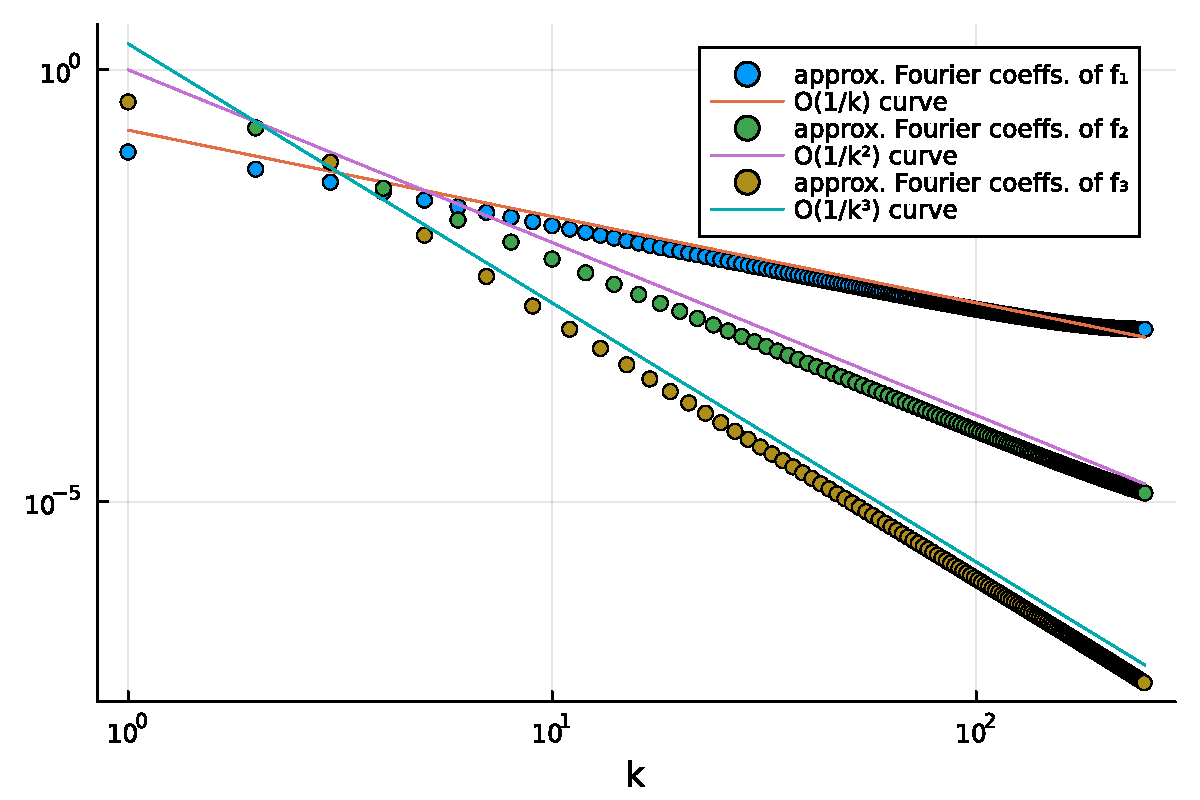
\includegraphics[width=\linewidth]{jl_fFQb2q/Fourier_24_1.pdf}

\begin{lstlisting}
(*@\HLJLn{p}@*)
(*@\HLJLn{f\ensuremath{\_4}}@*) (*@\HLJLoB{=}@*) (*@\HLJLn{x}@*) (*@\HLJLoB{->}@*) (*@\HLJLnf{exp}@*)(*@\HLJLp{(}@*)(*@\HLJLoB{-}@*)(*@\HLJLni{1}@*)(*@\HLJLoB{/}@*)(*@\HLJLnf{sin}@*)(*@\HLJLp{(}@*)(*@\HLJLn{x}@*)(*@\HLJLoB{/}@*)(*@\HLJLni{2}@*)(*@\HLJLp{)}@*)(*@\HLJLoB{{\textasciicircum}}@*)(*@\HLJLni{2}@*)(*@\HLJLp{)}@*)
(*@\HLJLn{c\ensuremath{\_4}}@*) (*@\HLJLoB{=}@*) (*@\HLJLnf{fftshift}@*)(*@\HLJLp{(}@*)(*@\HLJLnf{fft}@*)(*@\HLJLp{(}@*)(*@\HLJLn{f\ensuremath{\_4}}@*)(*@\HLJLoB{.}@*)(*@\HLJLp{(}@*)(*@\HLJLn{x}@*)(*@\HLJLp{)))}@*)(*@\HLJLoB{/}@*)(*@\HLJLn{n}@*)
(*@\HLJLnf{scatter!}@*)(*@\HLJLp{(}@*)(*@\HLJLni{2}@*)(*@\HLJLoB{:}@*)(*@\HLJLni{2}@*)(*@\HLJLoB{:}@*)(*@\HLJLn{m}@*)(*@\HLJLp{,}@*)(*@\HLJLn{abs}@*)(*@\HLJLoB{.}@*)(*@\HLJLp{(}@*)(*@\HLJLn{c\ensuremath{\_4}}@*)(*@\HLJLp{[}@*)(*@\HLJLn{m}@*)(*@\HLJLoB{+}@*)(*@\HLJLni{2}@*)(*@\HLJLoB{:}@*)(*@\HLJLni{2}@*)(*@\HLJLoB{:}@*)(*@\HLJLk{end}@*)(*@\HLJLp{]),}@*)(*@\HLJLn{label}@*)(*@\HLJLoB{=}@*)(*@\HLJLs{"{}approx.}@*) (*@\HLJLs{Fourier}@*) (*@\HLJLs{coeffs.}@*) (*@\HLJLs{of}@*) (*@\HLJLs{f\ensuremath{\_4}"{}}@*)(*@\HLJLp{,}@*)(*@\HLJLn{legend}@*)(*@\HLJLoB{=:}@*)(*@\HLJLn{bottomleft}@*)(*@\HLJLp{)}@*)
\end{lstlisting}

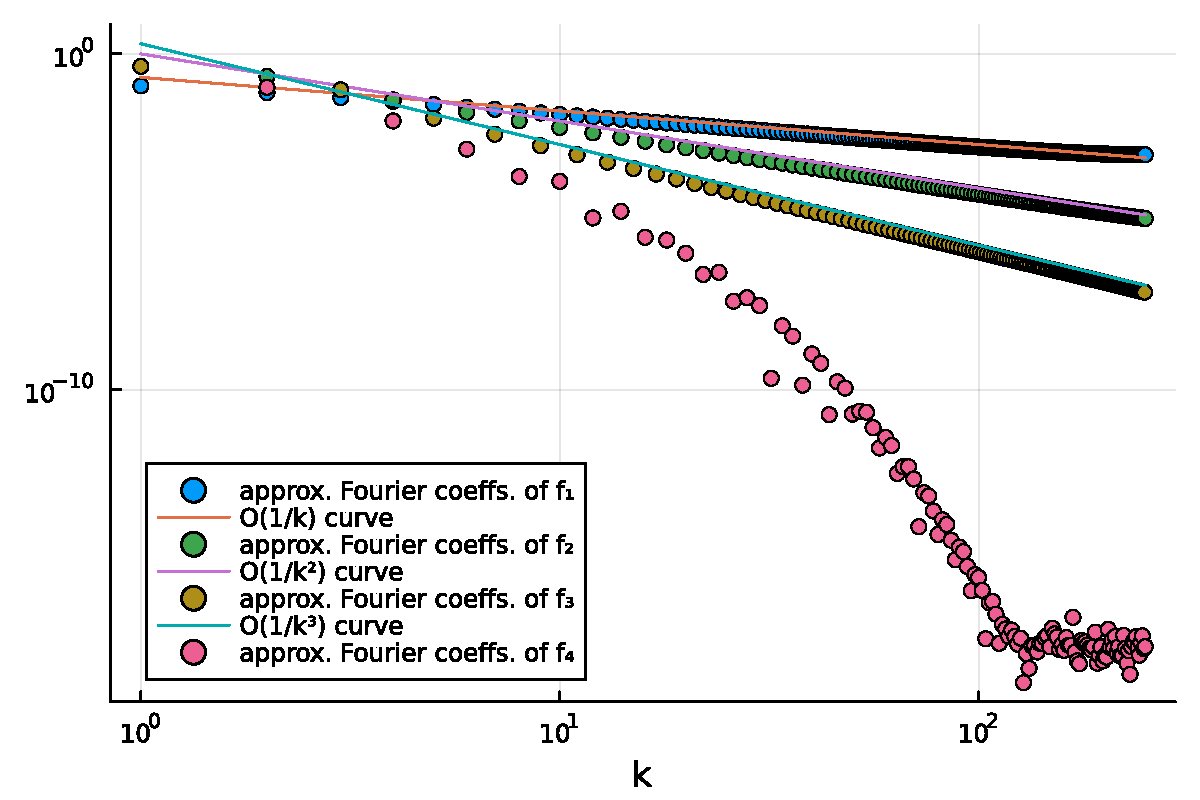
\includegraphics[width=\linewidth]{jl_fFQb2q/Fourier_25_1.pdf}

Functions that  are analytic on $[0, 2\pi]$ are even smoother than functions in $C^{\infty}[0, 2\pi]$ and consequently their Fourier coefficients decay even faster.

\textbf{Definition (analytic function)} A function $f(x)$ is analytic on a region $\Omega$ (think of a real interval $[a, b] \in \mathbb{R}$ or a region in the complex plane for those who have studied complex analysis) if its Taylor series has a positive radius of convergence for every $x \in \Omega$.

The Fourier coefficients of functions that are analytic on a neighbourhood of $[0, 2\pi]$ decay \emph{exponentially} fast.  To prove this and to quantify the rate of convergence, one needs to use techniques from complex analysis.  Since complex analysis is not a pre-requisite for this module, we won't prove this result.  Another fact that is proven in complex analysis is that the derivatives of analytic functions are also analytic functions! Here are two consequences:

\begin{itemize}
\item[1. ] If $f$ is analytic on $[0, 2\pi]$, then the approximate Fourier coefficients $\widetilde{c}_k$ (which we obtained via the trapezoidal rule) converge exponentially fast to the exact Fourier coefficients $c_k$ of $f$ as $n \to \infty$.   


\item[2. ] The trigonometric interpolant and its derivatives converge exponentially fast with $n$ to $f$ and its derivatives if $f$ is analytic.

\end{itemize}
A function $f(x)$ is called an \emph{entire function} if it is analytic on the entire complex plane; ${\rm e^{x}}$, $\cos x$ and $\sin x$ are examples of entire functions. The Fourier coefficients of entire functions decay at a \emph{super-exponential} rate.

A function $f(x)$ with $c_{k} = 0$ for $\vert k \vert > N$, where $N$ is a non-negative integer, is called a \emph{band-limited} function; $\cos x$ and $\sin x$ are examples of band-limited functions because $c_{k} = 0$ for $\vert k \vert > 1$ for these functions.

Here is an example of the decay of the approximate Fourier coefficients of a function in $C^{\infty}[0, 2\pi]$, an analytic function and an entire function. Note the plot below is on a semi-logarithmic scale.


\begin{lstlisting}
(*@\HLJLcs{{\#}}@*) (*@\HLJLcs{A}@*) (*@\HLJLcs{function}@*) (*@\HLJLcs{in}@*) (*@\HLJLcs{C{\textbackslash}{\textasciicircum}\ensuremath{\infty}[0,}@*) (*@\HLJLcs{2\ensuremath{\pi}]}@*)
(*@\HLJLnf{scatter}@*)(*@\HLJLp{(}@*)(*@\HLJLni{2}@*)(*@\HLJLoB{:}@*)(*@\HLJLni{2}@*)(*@\HLJLoB{:}@*)(*@\HLJLn{m}@*)(*@\HLJLp{,}@*)(*@\HLJLn{abs}@*)(*@\HLJLoB{.}@*)(*@\HLJLp{(}@*)(*@\HLJLn{c\ensuremath{\_4}}@*)(*@\HLJLp{[}@*)(*@\HLJLn{m}@*)(*@\HLJLoB{+}@*)(*@\HLJLni{2}@*)(*@\HLJLoB{:}@*)(*@\HLJLni{2}@*)(*@\HLJLoB{:}@*)(*@\HLJLk{end}@*)(*@\HLJLp{]),}@*)(*@\HLJLn{xlabel}@*)(*@\HLJLoB{=}@*)(*@\HLJLs{"{}k"{}}@*)(*@\HLJLp{,}@*)
(*@\HLJLn{yscale}@*)(*@\HLJLoB{=:}@*)(*@\HLJLn{log10}@*)(*@\HLJLp{,}@*)(*@\HLJLn{label}@*)(*@\HLJLoB{=}@*)(*@\HLJLs{"{}approx.}@*) (*@\HLJLs{Fourier}@*) (*@\HLJLs{coeffs.}@*) (*@\HLJLs{of}@*) (*@\HLJLs{f\ensuremath{\_4}"{}}@*)(*@\HLJLp{)}@*)
(*@\HLJLcs{{\#}}@*) (*@\HLJLcs{An}@*) (*@\HLJLcs{analytic}@*) (*@\HLJLcs{function}@*)
(*@\HLJLn{f\ensuremath{\_5}}@*) (*@\HLJLoB{=}@*) (*@\HLJLn{x}@*) (*@\HLJLoB{->}@*) (*@\HLJLni{1}@*)(*@\HLJLoB{/}@*)(*@\HLJLp{(}@*)(*@\HLJLnfB{1.2}@*) (*@\HLJLoB{-}@*) (*@\HLJLnf{sin}@*)(*@\HLJLp{(}@*)(*@\HLJLn{x}@*)(*@\HLJLp{))}@*)
(*@\HLJLn{c\ensuremath{\_5}}@*) (*@\HLJLoB{=}@*) (*@\HLJLnf{fftshift}@*)(*@\HLJLp{(}@*)(*@\HLJLnf{fft}@*)(*@\HLJLp{(}@*)(*@\HLJLn{f\ensuremath{\_5}}@*)(*@\HLJLoB{.}@*)(*@\HLJLp{(}@*)(*@\HLJLn{x}@*)(*@\HLJLp{)))}@*)(*@\HLJLoB{/}@*)(*@\HLJLn{n}@*)
(*@\HLJLnf{scatter!}@*)(*@\HLJLp{(}@*)(*@\HLJLni{1}@*)(*@\HLJLoB{:}@*)(*@\HLJLn{m}@*)(*@\HLJLp{,}@*)(*@\HLJLn{abs}@*)(*@\HLJLoB{.}@*)(*@\HLJLp{(}@*)(*@\HLJLn{c\ensuremath{\_5}}@*)(*@\HLJLp{[}@*)(*@\HLJLn{m}@*)(*@\HLJLoB{+}@*)(*@\HLJLni{2}@*)(*@\HLJLoB{:}@*)(*@\HLJLk{end}@*)(*@\HLJLp{]),}@*)(*@\HLJLn{label}@*)(*@\HLJLoB{=}@*)(*@\HLJLs{"{}approx.}@*) (*@\HLJLs{Fourier}@*) (*@\HLJLs{coeffs.}@*) (*@\HLJLs{of}@*) (*@\HLJLs{f\ensuremath{\_5}"{}}@*)(*@\HLJLp{)}@*)
(*@\HLJLcs{{\#}}@*) (*@\HLJLcs{An}@*) (*@\HLJLcs{entire}@*) (*@\HLJLcs{function}@*)
(*@\HLJLn{f\ensuremath{\_6}}@*) (*@\HLJLoB{=}@*) (*@\HLJLn{x}@*) (*@\HLJLoB{->}@*) (*@\HLJLnf{exp}@*)(*@\HLJLp{(}@*)(*@\HLJLnf{cos}@*)(*@\HLJLp{(}@*)(*@\HLJLni{10}@*)(*@\HLJLn{x}@*)(*@\HLJLp{))}@*)
(*@\HLJLn{c\ensuremath{\_6}}@*) (*@\HLJLoB{=}@*) (*@\HLJLnf{fftshift}@*)(*@\HLJLp{(}@*)(*@\HLJLnf{fft}@*)(*@\HLJLp{(}@*)(*@\HLJLn{f\ensuremath{\_6}}@*)(*@\HLJLoB{.}@*)(*@\HLJLp{(}@*)(*@\HLJLn{x}@*)(*@\HLJLp{)))}@*)(*@\HLJLoB{/}@*)(*@\HLJLn{n}@*)
(*@\HLJLnf{scatter!}@*)(*@\HLJLp{(}@*)(*@\HLJLni{0}@*)(*@\HLJLoB{:}@*)(*@\HLJLn{m}@*)(*@\HLJLp{,}@*)(*@\HLJLn{abs}@*)(*@\HLJLoB{.}@*)(*@\HLJLp{(}@*)(*@\HLJLn{c\ensuremath{\_6}}@*)(*@\HLJLp{[}@*)(*@\HLJLn{m}@*)(*@\HLJLoB{+}@*)(*@\HLJLni{1}@*)(*@\HLJLoB{:}@*)(*@\HLJLk{end}@*)(*@\HLJLp{]),}@*)(*@\HLJLn{label}@*)(*@\HLJLoB{=}@*)(*@\HLJLs{"{}approx.}@*) (*@\HLJLs{Fourier}@*) (*@\HLJLs{coeffs.}@*) (*@\HLJLs{of}@*) (*@\HLJLs{f\ensuremath{\_6}"{}}@*)(*@\HLJLp{)}@*)
\end{lstlisting}

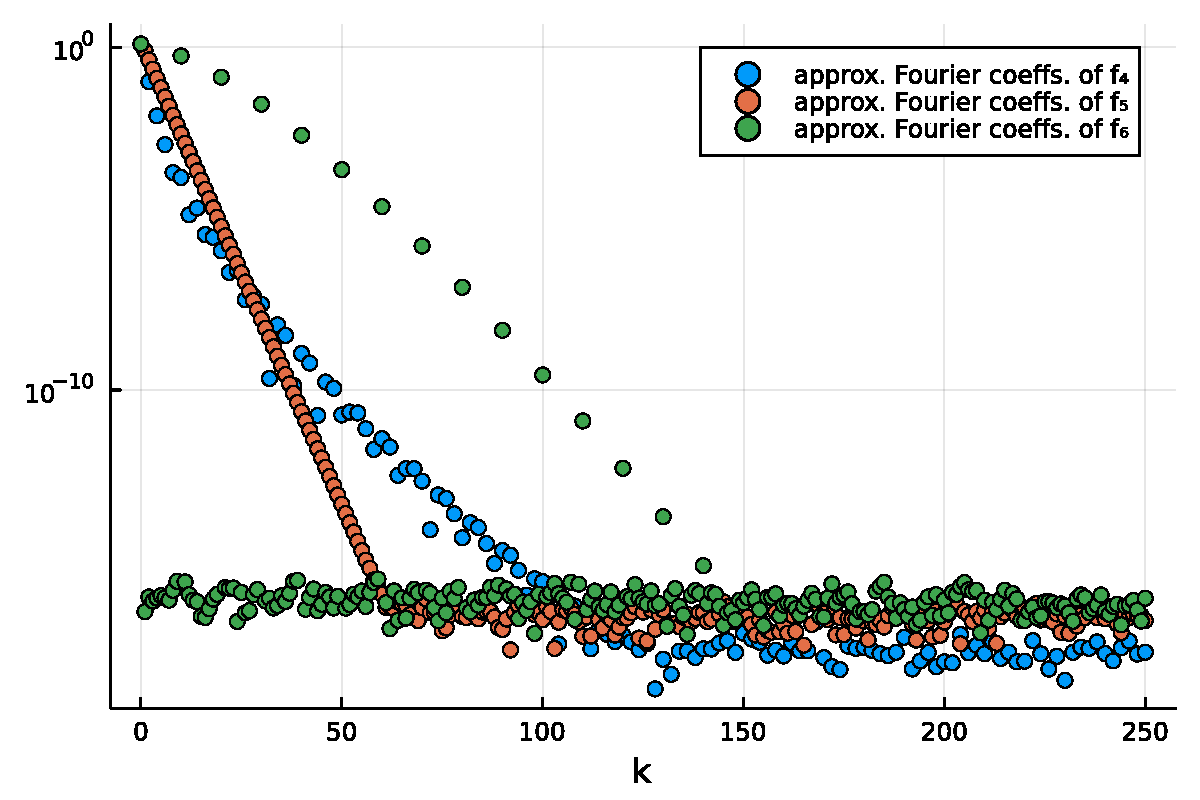
\includegraphics[width=\linewidth]{jl_fFQb2q/Fourier_26_1.pdf}


\end{document}
